% !TEX TS-program = pdflatex
%%%%%%%%%%%%%%%%%%%%%%%%%%%%%%%%%%%%%%%%%%%%%%%%%%%%%%%%%%%%%%%
%
%     filename  = "YourName-Dissertation.tex",
%     version   = "1.6.5",
%     date      = "2019/07/10",
%     authors   = "Gary L. Gray,
%     copyright = "Gary L. Gray",
%     address   = "Engineering Science and Mechanics,
%                  212 Earth & Engineering Sciences Bldg.,
%                  Penn State University,
%                  University Park, PA 16802,
%                  USA",
%     telephone = "814-863-1778",
%     email     = "gray@psu.edu",
%
%%%%%%%%%%%%%%%%%%%%%%%%%%%%%%%%%%%%%%%%%%%%%%%%%%%%%%%%%%%%%%%
% Change History:
% The change history can be found in the accompanying document
% entitled "YourName-Dissertation Template Change History.md".
%%%%%%%%%%%%%%%%%%%%%%%%%%%%%%%%%%%%%%%%%%%%%%%%%%%%%%%%%%%%%%%
%
% This is a template file to help get you started using the
% psuthesis.cls for theses and dissertations at Penn State
% University. You will, of course, need to put the
% psuthesis.cls file someplace that LaTeX will find it.
%
% I have set up a directory structure that I find to be clean
% and convenient. You can readjust it to suit your tastes. In
% fact, the structure used by our students is even a little
% more involved and commands are defined to point to the
% various directories.
%
% This document has been set up to be typeset using pdflatex.
% About the only thing you will need to change if typesetting
% using latex is the \DeclareGraphicsExtensions command.
%
% The psuthesis document class uses the same options as the
% book class. In addition, it requires that you have the
% ifthen, calc, setspace, and tocloft packages.
%
% The first additional option specifies the degree type. You
% can choose from:
%	Ph.D. using class option <phd>
%	M.S. using class option <ms>
%	M.Eng. using class option <meng>
%	M.A. using class option <ma>
%	B.S. using class option <bs>
%	B.A. using class option <ba>
%	Honors from the Schreyer Honors College <schreyer>
%
% The second additional option inlinechaptertoc determines
% the formatting of the Chapter entries in the Table of
% Contents. The default sets them as two-line entries (try it).
% If you want them as one-line entries, issue the
% inlinechaptertoc option.
%
% The class option schreyer should be used for theses
% submitted to the Schreyer Honors College.
%
% The class option esc should be used by all Engineering Science
% students.
%
% The option option twoha should be used if you are earning
% interdisciplanary honors and thus have two honors advisors.
%
% The class option ``secondthesissupervisor'' should be used
% for baccalaureate honors degrees if you have a second
% Thesis Supervisor.
%
% The vita is only included with the phd option and it is
% placed at the end of the thesis. The permissions page is only
% included with the ms, meng, and ma options.
%%%%%%%%%%%%%%%%%%%%%%%%%%%%%%%%%%%%%%%%%%%%%%%%%%%%%%%%%%%%%%%
% Only one of the following lines should be used at a time.
% Doctoral students.
%\documentclass[phd,12pt]{psuthesis}
% Masters students
%\documentclass[ms,12pt]{psuthesis}
% Bachelors students in the Schreyer Honors College.
\documentclass[phd,12pt]{psuthesis}
% Bachelors students in the Schreyer Honors College & Engineering Science.
%\documentclass[bs,schreyer,esc,twoha,12pt]{psuthesis}
% Bachelors students in Engineering Science.
%\documentclass[bs,esc,12pt]{psuthesis}

\usepackage[T1]{fontenc}
\usepackage{lmodern}
\usepackage{textcomp}
\usepackage{microtype}

%%%%%%%%%%%%%%%%%%%%%%%%%%%
% Packages I like to use. %
%%%%%%%%%%%%%%%%%%%%%%%%%%%
\usepackage{amsmath}
\usepackage{amssymb}
%\usepackage{amsthm}
%\usepackage{exscale}
%\usepackage[mathscr]{eucal}
%\usepackage{bm}
\usepackage{subfigure}
\usepackage{eqlist} % Makes for a nice list of symbols.
\usepackage[nosepfour,warning,np,debug,autolanguage]{numprint}
\usepackage{acro}
\usepackage{booktabs}
\usepackage[final]{graphicx}
\usepackage[dvipsnames]{color}
\DeclareGraphicsExtensions{.pdf, .jpg}
\usepackage{listings}
\usepackage{times}
\usepackage{soul}
\usepackage{url}
\usepackage{caption}
\usepackage{graphicx}
\usepackage{amsmath}
\usepackage{amsthm}
\usepackage{booktabs}
\usepackage{adjustbox}
\usepackage{algorithm}
\usepackage{algorithmic}
\usepackage{pifont}% http://ctan.org/pkg/pifont
\usepackage{float}
\usepackage{placeins}
\usepackage{balance}
\usepackage{diagbox}
\usepackage{tikz}
\usetikzlibrary{calc,trees,positioning,arrows,fit,shapes,calc,trees}
\usepackage{xspace}
\usepackage{adjustbox}
\usepackage[font=small,labelfont=bf]{caption}
\usepackage[scaled]{beramono}
\usepackage[T1]{fontenc}
\usepackage[para,online,flushleft]{threeparttable}

\usepackage[english]{babel} % handle hyphenation
\usepackage{url}
\usepackage{fancybox}
\usepackage{float}


% http://www.tex.ac.uk/cgi-bin/texfaq2html?label=citesort
\usepackage{cite}

\usepackage{titlesec}
\newcommand{\cmark}{\ding{51}}%
\newcommand{\xmark}{\ding{55}}%
\let\oldemptyset\emptyset
\let\emptyset\varnothing

\lstset{
numbers=left,
frame=single,
language=C,
basicstyle=\fontfamily{fvm}\scriptsize,
showlines=true
%xleftmargin=.2\textwidth, xrightmargin=.2\textwidth,
}


%%%%%%%%%%%%%%%%%%%%%%%%%%%%%%%
% Use of the hyperref package %
%%%%%%%%%%%%%%%%%%%%%%%%%%%%%%%
%
% This is optional and is included only for those students
% who want to use it.
%
% To the hyperref package, uncomment the following line:
%\usepackage{hyperref}
%
% Note that you should also uncomment the following line:
%\renewcommand{\theHchapter}{\thepart.\thechapter}
%
% to work around some a problem hyperref has with the fact
% the psuthesis class has unnumbered pages after which page
% counters are reset.

% Set the baselinestretch using the setspace package.
% The LaTeX Companion claims that a \baselinestretch of
% 1.24 gives one-and-a-half line spacing, which is allowed
% by the PSU thesis office. As of October 18, 2013, the Graduate
% School states ``The text of an eTD may be single-, double- or
% one- and-a-half-spaced.'' Go nuts!
\setstretch{1.24}


%%%%%%%%%%%%%%%%%%%%%%%%%%%%%%%%%%%%
% SPECIAL SYMBOLS AND NEW COMMANDS %
%%%%%%%%%%%%%%%%%%%%%%%%%%%%%%%%%%%%
% Place user-defined commands below.

% Define the \acro command.
\makeatletter
\newif\ifFirstPar       \FirstParfalse
\def\smc{\sc}
\def\ninepoint{\small}
\DeclareRobustCommand\SMC{%
  \ifx\@currsize\normalsize\small\else
   \ifx\@currsize\small\footnotesize\else
    \ifx\@currsize\footnotesize\scriptsize\else
     \ifx\@currsize\large\normalsize\else
      \ifx\@currsize\Large\large\else
       \ifx\@currsize\LARGE\Large\else
        \ifx\@currsize\scriptsize\tiny\else
         \ifx\@currsize\tiny\tiny\else
          \ifx\@currsize\huge\LARGE\else
           \ifx\@currsize\Huge\huge\else
            \small\SMC@unknown@warning
 \fi\fi\fi\fi\fi\fi\fi\fi\fi\fi
}
\newcommand\SMC@unknown@warning{\TBWarning{\string\SMC: unrecognised
    text font size command -- using \string\small}}
\newcommand\textSMC[1]{{\SMC #1}}
\newcommand\acro[1]{\textSMC{#1}\@}

\makeatother

% command for vectors
\newcommand{\bv}[1]{\ensuremath{\vec{#1}}}
% command for unit vectors
\newcommand{\uv}[2][blank]{%
\ifthenelse{\equal{#1}{blank}}%
{\ensuremath{\hat{u}_{#2}}}%
{}%
%
\ifthenelse{\equal{#1}{.}}%
{\ensuremath{\dot{\hat{u}}_{#2}}}%
{}%
%
\ifthenelse{\equal{#1}{'}}%
{\ensuremath{\hat{u}'_{#2}}}%
{}%
}
\newcommand{\ui}{\ensuremath{\hat{\imath}}}
\newcommand{\uj}{\ensuremath{\hat{\jmath}}}
\newcommand{\uk}{\ensuremath{\hat{k}}}



%%%%%%%%%%%%%%%%%%%%%%%%%%%%%%%%%%%%%%%%%
% Renewed Float Parameters              %
% (Makes floats fit better on the page) %
%%%%%%%%%%%%%%%%%%%%%%%%%%%%%%%%%%%%%%%%%
\renewcommand{\floatpagefraction}{0.85}
\renewcommand{\topfraction}      {0.85}
\renewcommand{\bottomfraction}   {0.85}
\renewcommand{\textfraction}     {0.15}
\newcommand{\detect}{\textsf{Lorem}}
\newcommand{\tool}{\textsf{Abacus}}
\newcommand{\ctool}{\textsf{MME}}
\newcommand{\framework}{\textsf{Phoenix}}
% ----------------------------------------------------------- %
\newtheorem{mydef}{Definition}
\newtheorem{theorem}{Theorem}
%%%%%%%%%%%%%%%%
% FRONT-MATTER %
%%%%%%%%%%%%%%%%
% Title
\title{Precise and Scalable Side-Channel Analysis}

% Author and Department
\author{Qinkun Bao}
\dept{College of Information Sciences and Technology}
% the degree will be conferred on this date
\degreedate{May 2021}
% year of your copyright
\copyrightyear{2021}

% This command is used for students submitting a thesis to the
% Schreyer Honors College and for students in Engineering Science.
% The argument of this command should contain every after the word
% ``requirements'' that appears on the title page. This provides the
% needed flexibility for all the degree types.
%\bachelorsdegreeinfo{for a baccalaureate degree \\ in Engineering Science \\ with honors in Engineering Science}

% This is the document type. For example, this could also be:
%	Comprehensive Document
%	Thesis Proposal
%\documenttype{Thesis}
\documenttype{Dissertation}
%\documenttype{Comprehensive Document}


% This will generally be The Graduate School, though you can
% put anything in here to suit your needs.
\submittedto{The Graduate School}

% This is the college to which you are submitting the
% thesis/dissertation.
\collegesubmittedto{College of Information Sciences and Technology}


%%%%%%%%%%%%%%%%%%
% Signatory Page %
%%%%%%%%%%%%%%%%%%
% You can have up to 7 committee members, i.e., one advisor
% and up to 6 readers.
%
% Begin by specifying the number of readers.
\numberofreaders{5}

% For baccalaureate honors degrees, enter the name of your
% honors advisor below.
%\honorsadvisor{Honors P. Advisor}
%{Associate Professor of Engineering Science and Mechanics}
%\honorsadvisortwo{Honors P. Advisor, Jr.}
%{Professor of Engineering Science and Mechanics}

% For baccalaureate honors degrees, if you have a second
% Thesis Supervisor, enter his or her name below.
%\secondthesissupervisor{Second T. Supervisor}

% For baccalaureate honors degrees, certain departments
% (e.g., Engineering Science and Mechanics) require the
% signature of the department head. In that case, enter the
% name and title of your department head below.
%\escdepthead{Department Q. Head}
%\escdeptheadtitle{P. B. Breneman Chair and Professor 
%of Engineering Science and Mechanics
%}

% Input reader information below. The optional argument, which
% comes first, goes on the second line before the name.
\advisor[Thesis Advisor][Chair of Committee]
		{Dinghao Wu}
		{Associate Professor of Information Sciences and Technology}

\readerone[The Pennsylvania State University]
			{Peng Liu}
			{Professor of Information Sciences and Technology}

\readertwo[The Pennsylvania State University]
			{Benjamin V. Hanrahan}
			{Assistant Professor of Information Sciences and Technology}

\readerthree[The Pennsylvania State University]
			{Sencun Zhu}
			{Associate Professor of Computer Science and Engineering}

\readerfour[EPFL]
			{James R. Larus}
			{Professor and Dean of the School of Computer and Communication Sciences}

\readerfive[The Pennsylvania State University]
			{Mary Beth Rosson}
			{Director of Graduate Programs and Professor of Information Sciences and Technology}

% Format the Chapter headings using the titlesec package.
% You can format section headings and the like here too.
\definecolor{gray75}{gray}{0.75}
\newcommand{\hsp}{\hspace{15pt}}
\titleformat{\chapter}[display]{\fontsize{30}{30}\selectfont\bfseries\sffamily}{Chapter \thechapter\hsp\textcolor{gray75}{\raisebox{3pt}{|}}}{0pt}{}{}

\titleformat{\section}[block]{\Large\bfseries\sffamily}{\thesection}{12pt}{}{}
\titleformat{\subsection}[block]{\large\bfseries\sffamily}{\thesubsection}{12pt}{}{}


% Makes use of LaTeX's include facility. Add as many chapters
% and appendices as you like.
\includeonly{%
Chapter-1/Chapter-1,%
Chapter-2/Chapter-2,%
Chapter-3/Chapter-3,%
Chapter-4/Chapter-4,%
Chapter-5/Chapter-5,%
Chapter-6/Chapter-6,
Appendix-A/Appendix-A,%
Appendix-B/Appendix-B
}

\usepackage{listings}
%%%%%%%%%%%%%%%%%
% THE BEGINNING %
%%%%%%%%%%%%%%%%%
\begin{document}
\pagestyle{fancy}
\fancyhead[L,C,R]{}
\fancyfoot[L,R]{}
\fancyfoot[C]{\thepage}
\renewcommand{\headrulewidth}{0pt}
\renewcommand{\footrulewidth}{0pt}
%%%%%%%%%%%%%%%%%%%%%%%%
% Preliminary Material %
%%%%%%%%%%%%%%%%%%%%%%%%
% This command is needed to properly set up the frontmatter.
\frontmatter

%%%%%%%%%%%%%%%%%%%%%%%%%%%%%%%%%%%%%%%%%%%%%%%%%%%%%%%%%%%%%%
% IMPORTANT
%
% The following commands allow you to include all the
% frontmatter in your thesis. If you don't need one or more of
% these items, you can comment it out. Most of these items are
% actually required by the Grad School -- see the Thesis Guide
% for details regarding what is and what is not required for
% your particular degree.
%%%%%%%%%%%%%%%%%%%%%%%%%%%%%%%%%%%%%%%%%%%%%%%%%%%%%%%%%%%%%%
% !!! DO NOT CHANGE THE SEQUENCE OF THESE ITEMS !!!
%%%%%%%%%%%%%%%%%%%%%%%%%%%%%%%%%%%%%%%%%%%%%%%%%%%%%%%%%%%%%%

% Generates the title page based on info you have provided
% above.
\psutitlepage

% Generates the committee page -- this is bound with your
% thesis. If this is an baccalaureate honors thesis, then
% comment out this line.
\psucommitteepage

% Generates the abstract. The argument should point to the
% file containing your abstract. 
\thesisabstract{SupplementaryMaterial/Abstract}

% Generates the Table of Contents
\thesistableofcontents

% Generates the List of Figures
\begin{singlespace}
\renewcommand{\listfigurename}{\sffamily\Huge List of Figures}
\setlength{\cftparskip}{\baselineskip}
\addcontentsline{toc}{chapter}{List of Figures}
%\fancypagestyle{plain}{%
%\fancyhf{} % clear all header and footer fields
%\fancyfoot[C]{\thepage}} % except the center
\listoffigures
\end{singlespace}
\clearpage

% Generates the List of Tables
\begin{singlespace}
\renewcommand{\listtablename}{\sffamily\Huge List of Tables}
\setlength{\cftparskip}{\baselineskip}
\addcontentsline{toc}{chapter}{List of Tables}
\listoftables
\end{singlespace}
\clearpage

% Generates the List of Symbols. The argument should point to
% the file containing your List of Symbols. 
%\thesislistofsymbols{SupplementaryMaterial/ListOfSymbols}

% Generates the Acknowledgments. The argument should point to
% the file containing your Acknowledgments. 
\thesisacknowledgments{SupplementaryMaterial/Acknowledgments}

% Generates the Epigraph/Dedication. The first argument should
% point to the file containing your Epigraph/Dedication and
% the second argument should be the title of this page. 
%\thesisdedication{SupplementaryMaterial/Dedication}{Dedication}



%%%%%%%%%%%%%%%%%%%%%%%%%%%%%%%%%%%%%%%%%%%%%%%%%%%%%%
% This command is needed to get the main part of the %
% document going.                                    %
%%%%%%%%%%%%%%%%%%%%%%%%%%%%%%%%%%%%%%%%%%%%%%%%%%%%%%
\thesismainmatter

%%%%%%%%%%%%%%%%%%%%%%%%%%%%%%%%%%%%%%%%%%%%%%%%%%
% This is an AMS-LaTeX command to allow breaking %
% of displayed equations across pages. Note the  %
% closing the "}" just before the bibliography.  %
%%%%%%%%%%%%%%%%%%%%%%%%%%%%%%%%%%%%%%%%%%%%%%%%%%
\allowdisplaybreaks{
%\pagestyle{fancy}
%\fancyhead{}
%
%%%%%%%%%%%%%%%%%%%%%%
% THE ACTUAL CONTENT %
%%%%%%%%%%%%%%%%%%%%%%
% Chapters
% !TEX root = ../YourName-Dissertation.tex

\chapter{Introduction} \label{chapter1:introduction}

Side channels are inevitable in modern computer systems as the sensitive
information may be leaked through many kinds of inadvertent behaviors, such as power, electromagnetic radiation, and even
sound~\cite{agrawal2002side,kar20178,chari1999towards,217605,genkin2014rsa}.
Among them, address-based side channel attacks, such as cache attacks, memory page attacks, and controlled-channel attacks, are especially common and have been studied for years~\cite{7163052,217543,217589,lee2017inferring,191010,liu2015last}. These
attacks result from vulnerable software and shared hardware components.
By observing program outputs or hardware behaviors, attackers can infer program
execution flows that manipulate secrets and guess secrets such as encryption
keys~\cite{Osvik2006,Gullasch:2011:CGB:2006077.2006784,203878,10.1007/978-3-540-45238-6_6}.

In this chapter, we first introduce two code patterns that can be exploited to retrieve sensitive information. After that, we discuss some common attacks and corresponding defense strategies. The limitations of existing work motivate the research in the dissertation. Finally, we summarize the contributions of the dissertation.

\section{Address-based Side-channel}
\subsection{Attack}
Address-based side-channel attacks happen when a program has different behaviors when it accesses different memory addresses. Most of the attack allows the attacker to shares some hardware resources (e.g., CPU Cache, TLB, and DRAM) with the victim. As a result, while the root reason of the attack is the same, there are various approaches that can exploit the attack at different granularities. 

Cache channels rely on the time difference between cache misses and cache hits. A cache channel works when the victim program and the attacker's program shares some sized chunks like cache lines or cache sets. Recent studies shows that an attacker can even observe the address access at a finer granularity (e.g., CacheBleed). Page-level side-channels allow attackers observe the memory access at the granularity of memory pages. 

In this dissertation, we consider three types of granularity: byte (1 Byte), cache line size (64 Bytes), page size (4 KBs). To the best of our knowledge, the three types of granularities can cover most of the side-channel attacks in literature.

When we examine those side-channel attacks, many of them stem from the two code patterns, \emph{secret-dependent control-flow transfers} and \emph{secret-dependent data accesses}.
\begin{figure}[h]
\begin{lstlisting}[xleftmargin=.32\textwidth, xrightmargin=.32\textwidth]
int secret[32];
...
while(i>0){
    r = (r * r) % n;
    if(secret[--i] == 1)
        r = (r * x) % n;   
}
\end{lstlisting}
\caption{Secret-dependent control-flow transfers}
\label{fig:secret:cf}
\end{figure}

Secret-dependent control-flow transfers happen when the value of secret can affect which branch the code executes. Figure~\ref{fig:secret:cf} shows an example. Depending on the value of \textsf{secret}, the code may or may not execute the code at line 6. As attackers, they can retrieve some information based on the execution control-flow. 

\begin{figure}[h]
\begin{lstlisting}[xleftmargin=.32\textwidth, xrightmargin=.32\textwidth]
static char FSb[256] = {...}
... 
uint32_t a = *RK++ ^ \ 
(FSb[(secret)) ^
(FSb[(secret >> 8)] << 8 ) ^
(FSb[(secret >>16)] << 16 ) ^
(FSb[(secret >>24)] << 24 );
...
\end{lstlisting}
\caption{Secret-dependent data accesses}
\label{fig:secret:da}
\end{figure}

Secret-dependent data accesses happen when the value of the secret can affect which memory cell the code reads or writes. Figure~\ref{fig:secret:da} shows an example. \textsf{FSb} is an array. Depending on the value of \textsf{secret}, the code may read or write different items in the array. 

\subsection{Defense}



Both hardware~\cite{Page2005PartitionedCA,
Wang:2007:NCD:1250662.1250723,Zhang:2015:HDL:2775054.2694372,Li:2014:SLH:2541940.2541947,
236344, 236334} and software~\cite{shih2017t,Coppens:2009:PMT:1607723.1608124,
brickell2006software,crane2015thwarting, 197207} side-channels mitigation techniques have
been proposed recently. Hardware countermeasures, including partitioning hardware resources~\cite{Page2005PartitionedCA}, randomizing cache
accesses~\cite{Wang:2007:NCD:1250662.1250723, 236344}, and designing new
architecture~\cite{tiwari2011crafting}, require changes to complex processors and are complex to adopt. 

On the contrary, software approaches are
usually easy to implement. By removing the above two kinds of code patterns, developers protect their 
code from a seris of side-channel attacks.
Coppens et
al.~\cite{Coppens:2009:PMT:1607723.1608124} uses a compiler
to eliminate key-dependent control-flow transfers. Crane et
al.~\cite{crane2015thwarting} mitigated side-channels by randomizing software.
As for crypto libraries, the basic idea is to eliminate key-dependent
control-flow transfers and data accesses. Common approaches include
bit-slicing~\cite{konighofer2008fast,rebeiro2006bitslice} and unifying
control-flows~\cite{Coppens:2009:PMT:1607723.1608124}.




Regarding the root cause of software-based side channel attacks, many of them originate
from two specific circumstances: data flow from secrets to load
addresses and data flow from secrets to branch conditions. We refer to them as
 secret-dependent memory-access and control-flow, respectively. A
central problem is eliminating these two code patterns. 
Recent
works~\cite{203878,217537,Wichelmann:2018:MFF:3274694.3274741,Brotzman19Casym,236338,182946},
find plenty of side-channel vulnerabilities. For example,
DATA~\cite{217537} reports 2,246 potential leakage sites for the RSA
implementation in OpenSSL\@. 
%After some inspections, 1,510 leakages are dismissed. But it
%still leaves 460 data-access leakages and 278 control-flow leakages. 
However, we find most of the reported vulnerabilities are not fixed because
of the following reasons.
First, many side-channels vulnerable implementations have better performance.
Those vulnerabilities are well-known for years. For example,
Symmetric encryptions like AES and DES still uses lookup tables (T-tables), which
is fast but notoriously known to be vulnerable to side channels.
As for asymmetric encryptions, most implementations of RSA, adopt the CRT optimization,
which is faster but vulnerable to fault attacks~\cite{aumuller2002fault}.
Second, side-channels are numerous and it is hard to fix all these vulnerabilities,
let alone the majority of them are negligible. 
That is, some vulnerabilities can result in the key being 
entirely compromised~\cite{184415, aumuller2002fault}, but many other vulnerabilities prove to be less
severe in reality. Therefore, we need a proper quantification metric to 
assess the sensitive level of side-channel vulnerabilities.

Previous attempts like static methods~\cite{182946,5207642}, usually with
abstract interpretations, can give a leakage upper bound, which is useful to
justify the implementation is secure if they report zero or little leakage.
However, they cannot indicate how severe the leakage is because of the
over-approximation method they apply. For example, CacheAudit~\cite{182946} reports that the upper
bound leakage of AES-128 exceeds the original key size! The dynamic methods take
another approach with a concrete input and run the program in a real
environment. Although they are very precise in terms of actual leakages, no
existing tool can precisely assess the severity of the vulnerabilities in production
software. 

To overcome these limitations, we propose a novel method to quantify information
leakages precisely. Unlike previous works that only consider the
``average'' information leakage, we study the problem based on real attack
scenarios. The average information leakage model assumes the target program has
\emph{variable} or \emph{random} sensitive information as inputs when an attack is
launched. However, for real-world attacks, an adversary may run the target
problem with the \emph{fixed} unknown sensitive information
as the input. Therefore, the previous threat model cannot model real attack
scenarios. In contrast, our method is more precise and fine-grained. 
We quantify
the amount of leaked information as the cardinality of the set of possible
inputs based on attackers' observations.
Before an attack, an adversary has a large but finite input space. Every time
when the adversary observes a leakage site, he can eliminate some potential
inputs and reduce the size of the input space. The smaller the input space is,
the more information is obtained. In an extreme case, if the size of the
input space reduces to one, the adversary can uniquely determine the input, 
which means all the secret information (e.g., the whole secret key) is
leaked. By counting the number of distinct inputs, we can quantify the
information leakage precisely.

We use constraints generated from symbolic execution to model the relation 
between the original sensitive input
and the attacker's observations. Symbolic execution can
provide fine-grained information but is usually believed to be an expensive
operation in terms of performance. Therefore, existing dynamic symbolic
execution works~\cite{203878,236338,Brotzman19Casym} either only analyze
small programs or apply some domain knowledge~\cite{203878} to simplify the analysis. We
systematically exam the bottleneck of the trace-oriented symbolic execution and optimize it
to be scalable to real-world cryptosystems.

We apply the above technique and build a tool called \tool{},
%\footnote{CleverHans is a horse that can ``count''. Our tool uses an advanced
%%method to count the number of leaked bits from side channels.} 
to discover potential information leakage sites as well as estimate how
many bits they can leak for each leakage site. 
First, we collect dynamic execution traces for each target
libraries and then run symbolic execution on each instruction. In this way, we model
each side-channel leakage as a logic formula. The sensitive input is divided into
several independent bytes, and each byte is regarded as a unique and free symbol. Those
formulas can precisely model side-channel vulnerabilities. Then we use the conjunction
of those formulas to model the same leaks in the source code but appears in the different location of
the execution trace file (e.g., leakages inside a loop).
Finally, we introduce Monte Carlo
sampling method to estimate the single and combined information leakage. 

We apply \tool{} on both symmetric and asymmetric ciphers from real-world crypto
libraries, including OpenSSL, mbed TLS and Monocypher\@. The experimental result confirms
that \tool{} can precisely identify previously known vulnerabilities, report
how much information is leaked and which byte in the original sensitive buffer
is leaked. We also test \tool{} on side-channel free algorithms. \tool{} has no
false positives.
Although some of the analyzed crypto libraries have a number of
side-channels, they actually leak very little information. Also, we also show the
of widely deployed software countermeasures can mitigate side channels.
\tool\ also discovers new vulnerabilities. With the help of \tool{}, we confirm
that those vulnerabilities are severe.

In summary, we make the following contributions:

\begin{itemize}
      \item We propose a novel method that can quantify fine-grained leaked
            information from side-channel vulnerabilities to match real attack
            scenarios. Our method is different from previous ones in that we
            model real attack scenarios more precisely, while the previous
            research only models the ``average'' or ``random'' case. 
            We transfer the information quantification problem into a counting
            problem and use the Monte Carlo sampling method to estimate the
            information leakage.
            % compared to previous results and
            %%   We model each side-channel vulnerabilities as math formulas %
            %and mutiple side-channel vulnerabilities can be seen as the %
            %conjunction of those formulas, which precisely models the % program
            %semantics.

      %%\item  Some initial results indicate the sampling
      %%     method suffers from the curse of dimensionality problem. Therefore, we
      %%      design a guided sampling method and provide the
      %%      corresponding error estimate.

      \item We implement the proposed method into a practical tool and apply it
            on several real-world software. \tool{} successfully identifies
            memory-related side-channel vulnerabilities and calculates the
            corresponding information leakage. 
            Our results are surprisingly different, much more useful in practice.
            The information leakage results
            provide detailed information that can help developers to fix the
            reported vulnerabilities.
\end{itemize}



\section{Contribution}


\section{Dissertation Organization}
The rest of the dissertation is organized as follows. We first present relevant backgrounds and related works in Chapter~\ref{chapter1}. We then propose our works in
Chapter~\ref{chapter2}. Chapter~\ref{chapter3} and Chapter~\ref{chapter4} introduce
our recent progress about the proposed work. 

% !TEX root = ../YourName-Dissertation.tex

\chapter{Related Work}\label{chapter2}
This dissertation studies address-based side-channel attacks. We review the related work in this chapter. The related work covers the following aspects: side-channel attacks, detections, mitigation, information quantification, and current binary analysis tools.

\section{Side-channel Attacks}
While there are many kinds of side-channel attacks, we focus on address-based side-channel attacks in this dissertation.
Address-based side-channel attacks happen when a program accesses different memory locations as it processes different secrets. In modern computer systems, an attacker may share hardware resources (e.g., Cache, TLB, and DRAM) with the victim~\cite{ge2018survey,szefer2019survey}. An attacker can probe the shared hardware resource to infer the memory accesses of the victim. While the root cause of the attack is the same, there are many approaches, and an attacker can exploit side-channel leakage sites in different methods to retrieve the information at different granularities.

\begin{table}
    \centering
    \caption{Here are some representations of the vast side-channel attacks: the shared resources, the granularity of the attacker can observe, is there any published attacks on non-cryptography libraries, and if the type of attack has been used to exploit multiple leakage sites.}
    \label{table:side_channel_attack}
    \resizebox{\columnwidth}{!}{%

        \begin{tabular}{lllcc}
            \toprule
            Attacks                                           & Shared Resources & Granularity            & Non-Crpyto & Multiple \\ \midrule
            CacheBleed~\cite{yarom2017cachebleed}             & Cache            & Sub Cache Line (<64 B) & \xmark     & \xmark   \\
            CopyCat~\cite{moghimi2020copycat}                 & Page Tables      & Instruction            & \xmark     & \xmark   \\
            Prime + Probe~\cite{liu2015last}                  & Cache            & Cache Set (64-512 B)   & \cmark     & \xmark   \\
            Prime + Abort~\cite{disselkoen2017prime+}         & Cache            & Cache Set (64-512 B)   & \cmark     & \xmark   \\
            Flush + Reload~\cite{yarom2014flush+}             & Cache            & Cache Line (64 B)      & \cmark     & \cmark   \\
            Flush + Flush~\cite{gruss2016flush+}              & Cache            & Cache Line (64 B)      & \cmark     & \xmark   \\
            Controlled-channel Attack~\cite{xu2015controlled} & Page Tables      & Page (4 KB)            & \cmark     & \xmark   \\
            TLBleed~\cite{gras_translation_2018}              & MMUs             & TLB Set (4 KB)         & \cmark     & \xmark   \\
            Page Cache Attacks~\cite{gruss2019page}           & Page Cache       & Page (4 KB)            & \xmark     & \cmark   \\
            \bottomrule
        \end{tabular}
    }
\end{table}


Table~\ref{table:side_channel_attack} shows some representations of recent side-channel attacks. For a detailed overview of recent side-channel attacks, we refer to the survey paper by Ge et al.~\cite{ge2018survey}. We classified these side-channel attacks into two categories: cache-level channels and page-level channels.

\subsection{Cache-level Channel}
A CPU cache is an essential part of modern computer systems. It is a smaller and faster memory that is designed to reduce the average data access costs to the main memory by storing copies of data from the main memory. When a CPU reads data from a memory location, it first checks the cache. If it finds that the cache has a copy of data from the main memory, a cache hit occurs. Otherwise, the CPU needs to read from the main memory, and a cache miss happens.

Cache channels~\cite{yarom2017cachebleed,191010,184415,Osvik2006,liu2015last,184415} rely on the time difference between a cache miss and cache hit. The core-private caches (e.g., L1 and L2) are traditionally set-associate cache. The cache is divided into different cache sets, and each cache set is made up of several cache lines. Typically, the smallest storage unit in a CPU cache is a cache line. Cache channel attacks can observe cache accesses at the level of cache sets, cache lines or other granularities. We introduce two common attack strategies, namely Prime+Probe and Flush+Reload.

\textbf{Prime+Probe.} Prime+Probe targets a single cache set.
An attacker primes the cache set with its own data and waits until the victim executes the program. Then the attacker probes the cache by reading previously loaded data. If the victim accesses the cache set and evicts some lines of the data, the attacker will experience a slow measurement. Under the circumstance, the attacker can know that the victim must have touched some data that map to the same cache set.

\textbf{Flush+Reload.} Flush+Reload allows an attacker to observe memory accesses at the granularity of a cache line instead of a cache set. While Flush+Reload has a fine-grained granularity compared with Prime+Probe, it requires the attacker and victim to share some memory. It also has two stages. During the ``flush'' stage, the attacker flushes the ``monitored
memory'' from the cache and waits for the victim to access the memory, which may be a load of the sensitive information to the cache line.  In the next phase,
the attacker reloads the ``monitored memory''. The attacker's process read all data in the `monitored
memory''. If the time is relatively fast, it indicate that the data has been accessed by the victim program and the cache has loaded the data. 
On X86-64 machines, the two steps can be combined by measuring the time differences of the \textsf{clflush} instruction.

Based on the above attacks, some work~\cite{brickell2011technologies} suggests having secret-dependent memory accesses at finer than the size of one cache line should be secure enough. However, recent studies show that having different memory accesses within a cache line is also dangerous. One example is the CacheBleed attack~\cite{yarom2017cachebleed}. It is a cache channel attack that can exploit cache-bank collisions. 
\subsection{Page-level Channel}
Page channel attacks allow an attacker can observe the memory access at the granularity of memory pages. One example is the controlled-channel attack~\cite{xu2015controlled}. It is a primary threat to the trusted execution environments (TEEs).  A privileged adversary (e.g., kernel) can infer sensitive information by manipulating the enclave page accesses. A malicious OS can proactively revoke a virtual enclave memory page from the virtual memory. If the victim enclave program accesses the memory in the  page, then the OS can observe the page faults and know which page is accessed. While the granularity of controlled-channel attacks is more coarse-grained compared with cache channel attacks, controlled-channel attacks allow the attacker to have a noise-free observation. Other examples such as TLB side-channel attacks and DDRAM attacks share the same page-level granularity.


Based on the above discussion, we consider three types of granularities in the dissertation: byte (1 byte), cache line size (64 bytes), page size (4 KBs). To the best of our knowledge, these three types of granularities can cover most of the side-channel attacks in the literature.


\subsection{Attack Models}
Previous work~\cite{182946} classifies side-channel attacks into three types based on the type of information that an attacker can learn during an attack.
\subsubsection*{Timing-based Attacks}
In timing-based attacks, an adversary can measure and compare the execution time of victim programs. It could be the overall execution time or the execution time of some interesting components (e.g., a function).  The execution time is correlated to some events (e.g., cache hits and misses, page faults, the number of instructions, optimizations). Timing-based attacks are perilous because these attacks are able to be carried out remotely over the networks~\cite{brumley2005remote}. Examples of these attacks include remote timing attacks~\cite{brumley2005remote}, Bernstein's attack on AES~\cite{bernstein2005cache}, and Kocher’s original attack~\cite{kocher1996timing} from CRYPTO 96.
\subsubsection*{Access-based Attacks}
In access-based attacks, an adversary can learn the memory addresses that are accessed during the execution after the termination of the victim program. 
For example, a cache-based channel attack can know which memory access incurs a cache hit and which memory access incurs a cache miss to infer addresses that the victim program accesses. Since the attacker can probe the victim program after the execution, the attacker does not know the order of memory accesses. Access-based attacks often happen in the cloud computing environment when the attacker and victim share the same hardware (e.g., LLC cache). Examples of these attacks include cache template attacks~\cite{191010}, Prime+Probe attacks~\cite{liu2015last}, and Flush+Reload attacks~\cite{yarom2014flush+}.
\subsubsection*{Trace-based Attacks}
In trace-based attacks, an adversary can interrupt and  probe the victim program at any point. The attacker can learn the order of memory accesses. Suppose the victim program has two functions \textsf{a} and \textsf{b}. In an access-based attacks, the attacker can only learn both \textsf{a} and \textsf{b} are executed. In a trace-based attack, the attacker can know the execution sequence of two functions (e.g., $\mathtt{aabbb}$). Controlled-channel attacks~\cite{moghimi2020copycat, xu2015controlled} belong to this category where a malicious operating system can interrupt the victim application and probe the program at any time. In general, the trace-based attack has the strongest assumption about the threat model,  but it can retrieve more information compared to the other two types of attacks.
\subsection{Target Applications}
There is a large number of studies\cite{yarom2017cachebleed,191010,184415,Osvik2006,liu2015last} on side-channel attacks. Most early works targeted retrieving encryption keys from cryptography libraries. In recent years, researchers start to focus on more general and diverse applications. In summary,  the target applications of current side-channel attacks can be classified into three categories.

\subsubsection*{Cryptography Libraries}
\begin{table}
    \centering
    \caption{Some common vulnerable components in cryptography implementations and corresponding software mitigation methods.}
    \label{chapter2:table:crypto}
    \resizebox{\columnwidth}{!}{%

        \begin{tabular}{lll}
            \toprule
            Implementation & Common Vulnerable Point             & Mitigation \\ \midrule
            AES &  T-table and S-table lookups   & AES instructions (AES-NI) 
            \\&&Scalar bit-slicing \\&& Preloading tables     \\
            DES & Table lookups & Scalar bit-slicing (No implmentation) \\
            RSA & CRT optimization & Verifying the consistency with the public key\\
            & Modular exponentiation& Montgomery modular multiplication\\
            & & Base blinding and exponent blinding\\
            (EC)DSA & Scalar multiplication& Constant time scalar implementation\\
            &Modular inversion & Blinding\\
            &Modular reduction &\\
            \bottomrule
        \end{tabular}
        }
\end{table}

The first side-channel attack on cryptography libraries can be traced back to Kocher's timing attacks~\cite{kocher1996timing} in 1996. It exploits the simple modular exponentiation algorithm function in many cryptography (Diffie-Hellman, RSA) implementations. The function does not run in a fixed time. By measuring the time differences between the modular exponentiation algorithm computes the exponent bits (0 or 1), Kocher's attack can recover the whole secret key bit by bit. Since then, researchers start to break all kinds of cipher implementation through side-channel attacks.  Table~\ref{chapter2:table:crypto} summarizes some common vulnerable points in cryptography library implementations.  Note that cryptography libraries usually have several implementations for some ciphers.
For example, AES has more than five different implementations in OpenSSL. Depending on the build configuration and the return value of \textsf{CPUID}, the code may execute any implementation of them. The reference implementation usually adopts T-Tables and S-Tables to speed up the computation. However, such implementations are vulnerable to side-channels and can be exploited to retrieve the whole key~\cite{bonneau2006cache}. In addition to the reference implementation, these libraries also have side-channel mitigated versions. However, recent studies show these versions (e.g., AES-NI) also have side-channel vulnerabilities caused by compiler optimizations and human mistakes~\cite{217537}. The situation is even worse for asymmetric ciphers (e.g., Diffie-Hellman, RSA, ECDSA). These ciphers have a lot of big number calculations. It is hard to implement these calculations to be completely side-channel resistant. Recent work~\cite{arnaud2013timing,yarom2017cachebleed,yarom2014flush+} has demonstrated several end-to-end attacks to recover the private key of these ciphers. 

\subsubsection*{Machine Learning Applications}
Recent side-channel attacks on machine learning applications mainly focus on recovering two types of sensitive information: the input of the model and the architecture of deep learning models. Hua et al.~\cite{hua2018reverse} were the first in the literature to reverse engineer the architecture of convolutional neural networks (CNNs) through the memory access patterns. Wei et al.~\cite{wei2018know} perform the side-channel attacks on an FPG-based convolution neural network by using the power consumption to recover inputs to the networks. For an image classification task trained by the MNIST dataset, their attacks can achieve up to 89\% accuracy. CSI NN~\cite{batina2019csi} reverse engineered the multi-layer perception and convolution neural network based on the electromagnetic signals (EMs). Cache Telepathy~\cite{yan2020cache} introduces the cache-based side-channel attack to extract DNNs' architectures. We find that all existing approaches need a lot of domain knowledge and expertise to launch the attacks.

\subsubsection*{Media and Graphic Libraries}
Recent work also studies the side-channel attacks in media and graphic libraries. Gruss et at.~\cite{191010} show an attack that can infer keystrokes by exploiting secret-dependent memory accesses in the GDK library. In the controlled-channel attack~\cite{xu2015controlled}, Yuanzhong et al. demonstrate an attack to recover the outline of an image by exploiting the vulnerability in the inverse DCT function in libjpeg. Daimeng et al.~\cite{wang2019unveiling} present a cache attack on graphic libraries. Their approaches uses a machine learning approach to pick cache lines that can be exploited to leak the most information.
\subsubsection*{Others}
Some other side-channel targets also include spelling checking tools and font libraries~\cite{xu2015controlled}. The attack on font libraries is essentially the same as the attack on the graphic library GDK. By exploiting the differences of memory accesses when the program renders different characters, an attacker can recover parts of the original sensitive information. Other side-channel attacks target operating system kernels. One example is using the side-channel attack to break the kernel address space randomization (KASLR).
Many exploits rely on the knowledge of the memory location of a certain kernel function. Since Linux 4.12, the kernel loads core kernel image and device drivers at random positions during the boot time. Jang et al.~\cite{jang2016breaking} rely on side-channels to reveal the mapping status of each page. After that, they detect kernel modules with unique size signatures to break KASLR. The second example relies on the side-channel vulnerabilities~\cite{cao2019principled} inside kernels to infer the TCP sequence numbers, which can be used by a third party to hijack connections between the client and the server~\cite{cao2016off}.

\section{Defenses and Mitigation}

Both hardware~\cite{Page2005PartitionedCA,
    Wang:2007:NCD:1250662.1250723,Zhang:2015:HDL:2775054.2694372,Li:2014:SLH:2541940.2541947,
    236344, 236334} and software~\cite{shih2017t,Coppens:2009:PMT:1607723.1608124,
    brickell2006software,crane2015thwarting, 197207} side-channels mitigation techniques have
been proposed recently. Hardware countermeasures, including partitioning hardware resources~\cite{Page2005PartitionedCA}, randomizing cache
accesses~\cite{Wang:2007:NCD:1250662.1250723, 236344}, and designing new
architecture~\cite{tiwari2011crafting}, require changes to complex processors and are difficult to adopt. On the contrary, software approaches are
usually easy to implement. Coppens et
al.~\cite{Coppens:2009:PMT:1607723.1608124} use a compiler
to eliminate key-dependent control-flow transfers. Crane et
al.~\cite{crane2015thwarting} mitigate side-channels by randomizing software.
As for crypto libraries, the basic idea is to eliminate key-dependent
control-flow transfers and data accesses. Common approaches include
bit-slicing~\cite{konighofer2008fast,rebeiro2006bitslice} and unifying
control-flows~\cite{Coppens:2009:PMT:1607723.1608124}.

\subsection{Software Countermeasures}
\subsubsection*{Software Vulnerability Identification}
For many software countermeasures, the first step to identify side-channel leakages in software manually. It can be done manually or by some program analysis tools.
There are several existing works on side-channel leakage detections. As shown in Table~\ref{table:side_channel_detection_tool}, existing methods can be classified into two categories, tools based on the trace comparison and tools based on the abstraction.

\textbf{Trace comparison.} If a program has two different execution traces under two different sensitive inputs, then attackers can distinguish the sensitive input by observing the execution traces. Therefore, we can conclude the program is vulnerable to side-channel attacks. The method is similar to the UNIX tool \textsf{diff}.  The approach does not need to model or abstract the program's semantics. In general, the approach is quite fast. On the negative side, comparing the trace can find the leakage, but it cannot find the complex relationship between the leakage site and the original secret input. For example, if two leakage sites leak the same information, these approaches cannot find out the two leakages are the same.

\textbf{Abstraction.} The second category of these tools belongs to the field of abstractions. Tools based on these approaches use abstraction to generate approximations to model the semantics of computer programs. After that, by analyzing the model, these tools can identify side-channel leakages. Compared with the trace comparison approach, the method is more precise.

These methods usually follow the steps below. Suppose a program $P$ has $k$ as the input. These approaches first retrieve the relationship between the $k$ and temporary values during the execution. After that, they should have a cache or memory access model and model the side-channel leakage as a math constraint. By using SMT solvers to find different secret inputs that lead accesses to different locations in the memory or the cache, these approaches can determine if the program is vulnerable to side-channel attacks.
Unlike to the trace comparison, the method is quite precise. Moreover, it can model multiple leakages precisely as the conjunction of these formulas. However, these approaches have the following limitations.

\begin{itemize}
    \item Many tools can only analyze the source code or the intermediate representation level. However, side-channel are low-level problems in general.  Most existing tools are research prototypes. For some projects, the tools can only handle the benchmarks in their papers properly. 
    \item These tools heavily rely on SMT solvers. Despite SMT solvers having made incredible progress in performance, SMT solving is still the main bottleneck of these tools. SMT solvers are not good at non-linear arithmetic. However, non-linear arithmetics are quite common in cryptography algorithms.  Recent studies show existing solvers still have bugs when dealing with real number calculations. These calculations are also common in media libraries and machine learning applications.
\end{itemize}

According to Table~\ref{table:side_channel_detection_tool}, some methods may choose to analyze the source code or the intermediate representations of the vulnerable software. However, it still cannot solve the problem. First, many widely-used libraries (e.g., Intel MKL) do not provide source code. Second, some libraries use hard-coded assembly code to pursue maximum performance.
CacheAudit~\cite{182946} uses abstract domains to compute an
over-approximation of cache-based side-channel information leakage upper bound.
However, it is difficult to judge the sensitive level of the side-channel leakage based on the leakage provided by CacheAudit. Besides, CacheAudit is not scalable enough to analyze ciphers like RSA implementations. CacheS~\cite{236338} improves the approach from
CacheAudit with a new abstract model that only tracks
secret-related code. Like CacheAudit, CacheS cannot
measure the amount of leaked information in each side-channel vulnerability.
CaSym~\cite{Brotzman19Casym} introduces a static cache-aware symbolic reasoning technique to cover multiple paths in a target program. CaSym can work on two threat models: trace-based attacks and access-based attacks. Again, their
approaches cannot evaluate the sensitive level for each side-channel vulnerability, and it only works on small code snippets.

The dynamic approach, usually consisting of taint analysis and symbolic execution,
can perform a very precise analysis. CacheD~\cite{203878} takes a concrete execution trace and runs symbolic execution on the trace
to get a formula for each memory address. CacheD is
quite precise in avoiding false positives. However, CacheD is not able to detect secret-dependent control-flows. We adopted a similar approach to model the secret-dependent data accesses in the dissertation. \tool{} differs from CacheD in that we do not use traditional taint tracking or domain knowledge to cut the execution trace when identifying secret-dependent data access vulnerabilities. \tool{} works on machine instructions directly instead of intermediate representations. Moreover, \tool{} finds secret-dependent control-flows at the same time and gives a precise quantification of the leakage. DATA~\cite{217537} detects address-based side-channel vulnerabilities by comparing and aligning different execution traces under various test inputs. After collecting execution traces, DATA aligns them and finds the differences. It uses statistical hypothesis testing to find true leakages. However, both imperfect trace alignment and the statistical testing that DATA uses can produce false positives.
MicroWalk~\cite{Wichelmann:2018:MFF:3274694.3274741} adopts a similar approach as DATA by comparing all accessed addresses. It uses mutual information (MI) between sensitive input and execution state to quantify the information. 

\begin{sidewaystable}

    %\begin{table*}
    %\centering
    \caption{Many leakage detection tools are only evaluated on cryptography libraries.  All of them cannot reason about the total effect of multiple leakages.}
    \label{table:side_channel_detection_tool}
    \resizebox{1\columnwidth}{!}{%

        \begin{tabular}{lllcclc}
            \toprule
            Tool                                                 & S/D     & Method                              & AVX/SIMD & Multiple & Evaluation                                           & Available \\ \midrule
            CacheAudit~\cite{182946}                             & Static  & Abstraction                         & \xmark   & \xmark   & Crypto Algorithm                                     & \cmark    \\
            CacheD~\cite{203878}                                 & Dynamic & Symbolic Execution + Taint Analysis & \xmark   & \xmark   & Libgcrypt, OpenSSL                                   & \xmark    \\
            CachSym~\cite{Brotzman19Casym}                       & Static  & Symbolic Execution                  & \xmark   & \xmark   & Crypto Snippet                                       & \xmark    \\
            CacheS~\cite{236338}                                 & Static  & Abstract Interpretation             & \xmark   & \xmark   & Libgcrypt, OpenSSL, mbedTLS                          & \xmark    \\
            DATA~\cite{217537}                                   & Dynamic & Trace Alignment + Comparison        & \cmark   & \xmark   & OpenSSL, PyCrypto                                    & \cmark    \\
            ctgrind~\cite{langley2010ctgrind}                    & Dynamic & Taint Analysis                      & \cmark   & \xmark   & Crypto Library                                       & \cmark    \\
            Satcco~\cite{xiao2017stacco}                         & Dynamic & Trace Comparison                    & \cmark   & \xmark   & OpenSSL, GnuTLS, mbedTLS, WolfTLS, LibreSSL          & \xmark    \\
            ANABLEPS~\cite{wang2019time}                         & Dynamic & Trace Comparison                    & \cmark   & \xmark   & gsl, Hunspell, PNG, Freetype, QRcodegen, Genometools & \xmark    \\
            MicroWalk~\cite{Wichelmann:2018:MFF:3274694.3274741} & Dynamic & Trace Comparison                    & \cmark   & \xmark   & Intel IPP, Microsoft CNG                             & \cmark    \\
            \bottomrule
        \end{tabular}
    }
    %\end{table*}
\end{sidewaystable}

\subsubsection*{Software Patch}
Once we have identified side-channel leakages, there are two common approaches to mitigate side-channel attacks. The first approach is to adopt unified behavior code when computing the secret data. For example, a control flow leakage happens when different secret inputs lead to different paths. Software developers can mitigate the leakage by executing both branches and select the result with bit-wise operations~\cite{Coppens:2009:PMT:1607723.1608124}. However, for exiting code base, it is hard to migrate all the code into a side-channel free implementation. The second approach is to introduce randomized behaviors during the execution to obfuscate the information that an attacker can retrieve. One example is cryptographic blinding~\cite{coron1999resistance}. Developers can use a random value to blend the secret key but still generate the same encrypted data with a carefully designed algorithm.  Binding values can alter the program execution to some unpredictable states and introduce the randomization to the execution. However, the binding value can also be retrieved by an attacker through other methods, including side-channel attacks. An attacker can launch an attack to retrieve the binding value to recover the secret input.

\subsubsection{New Implementation}
Recent work~\cite{bernstein2012security,libsodium,zinzindohoue2017hacl} also proposes to design and implement clean-slate side-channel free software from scratch. 

\subsection{Hardware Countermeasures}
\subsubsection*{Resource Partitioning}
Side-channel attacks usually require attackers and victims to share some hardware resources (e.g., CPU cache, MMU). A straightforward way to defend these attacks is to partition the resources and ensure the attacker and the victim never share the same hardware resource~\cite{Page2005PartitionedCA,shi2011limiting,liu2016catalyst}. For example, in a cloud computing environment, several virtual machines (VMs) can be hosted on the same physical machine and these VMs share the same last-level cache (LLC). Researchers proposed different methods to partition the LLC such as cache coloring~\cite{shi2011limiting}, using Intel Cache Allocation Technology~\cite{liu2016catalyst}.
\subsubsection*{Randomization}
This type of defense randomizes the behaviors of hardware resources to make it harder for attackers to infer secrets based on side-channel information. For example, Random Permutation Cache ~\cite{wang2007new} uses a dynamically randomized memory to cache mapping table for each different process. Vattikonda et al.~\cite{vattikonda2011eliminating} add noises to the result of the system timer to mitigate timing-based channels.

\subsection{Discussion on Existing Countermeasures}
Despite a lot of hardware countermeasures that have been proposed in academia, few of them have been adopted in real-world production systems. In general, hardware countermeasures usually require new hardware designs and are harder to adopt in practice.  In addition, some hardware methods (e.g., Oblivious RAM) may introduce expensive computation overhead. Therefore, many practical solutions are still software countermeasures. However, software methods are not very general, and it is hard to find many side-channel leakages in large code bases manually. In this dissertation, we propose side-channel analysis methods to address the problem.
\section{Information Quantification}
Proposed by Denning~\cite{robling1982cryptography} and Gray~\cite{gray1992toward},
Quantitative Information Flow (QIF) aims to provide an estimation of the amount of leaked information from the sensitive information given the public output. If zero bits
of the information are leaked, the program is called non-interference. 
McCamant and Ernst~\cite{McCamantE2008} quantify the information leakage as the network
flow capacity. They model the possible information leakage as a network of limited-capacity
channel. After that, they use the maximum rate of the channel to represent the amount of secret information that the execution can reveal.
Backes et al.~\cite{5207642} propose an automated method for QIF
by computing an equivalence relation on the set of input keys. However,
the evaluation shows the approach only works on small programs.
Besides, their approach cannot handle programs with bitwise operations.
However, such bitwise operations are quite common in cryptographic libraries.
Phan et al.~\cite{Phan:2012:SQI:2382756.2382791} propose symbolic QIF. The goal of their
work is to ensure a program is non-interference. They adopt an over-approximation method to estimate the total information leakage, and their method
does not work for secret-dependent memory access side-channels.
Pasareanu et al.~\cite{pasareanu2016multi} combine symbolic analysis and Max-SMT solving to synthesize the concrete public input that can lead to the worst-case leakage. They assume the target program has multiple different input secrets and calculate the average leakage for one-fixed public input.
CHALICE~\cite{Chattopadhyay:2017:QIL:3127041.3127044} quantifies the leaked
information for a given cache behavior.
It symbolically reasons about cache
behavior and estimates the amount of leaked information based on cache miss/hit.
Their approach only scales to small programs, which limits its usage in
real-world applications. On the contrary, \tool{}~\cite{bao2021abacus} assesses the sensitive level
of side channels with different granularities. It can also analyze side channels in real-world cryptographic libraries.

Model counting refers to the problem of computing the number of satisfying
solutions for a propositional formula (\#SAT). There are two approaches to
solving the problem, exact model counting, and approximate model
counting. Exact model counting for propositional formulas (\#SAT) should determine
the number of solutions. Intuitively, such a model counter should traverse the whole
search space to find all the satisfying solutions. Consequently, the exact model counter is very slow. These model counters have difficulty in scaling up to real-world programs.
On the other hand, the approximate model counter is much faster compared with the exact model counter. The related work focuses on approximate model counting since it is close to our approach. Wei and Selman~\cite{wei2005new} introduce
ApproxCount, a local search-based method using Markov Chain Monte
Carlo (MCMC). ApproxCount has better scalability than
exact model counters. Other approximate model counter includes
SampleCount~\cite{gomes2007sampling},
Mbound~\cite{gomes2006model}, and MiniCount~\cite{kroc2008leveraging}.
Unlike ApproxCount, these model counters can give lower or upper bounds with guarantees.
Despite the rapid development of model counters for SAT and some
research~\cite{chistikov2017approximate,phan2015model}, existing tools cannot be directly applied to side-channel leakage quantification.
ApproxFlow~\cite{biondi2018scalable} uses ApproxMC~\cite{chakraborty2016algorithmic} for information flow quantification, but it has only been tested with small programs.

\section{Trace-based Binary Analysis}
Since our work relies on binary analysis, we briefly mention the related work here.
Trace-based binary analysis can be seen as a type of dynamic analysis. It analyzes one concrete program execution path each time rather than trying to cover
as many paths as possible. Compared to static analysis, trace-based analysis
is usually more precise as it can incorporate runtime information. It usually has
two steps. The first step is to collect trace information. Existing
approaches often rely on binary instrumentation frameworks or emulators (e.g., Intel Pin~\cite{luk2005pin},
Valgrind~\cite{nethercote2007valgrind}, and QEMU). The second step to analyze the trace using techniques, such
as symbolic execution and taint analysis. Depending on when the analysis is launched,
there are two kinds of trace-based analysis, online analysis and offline analysis. As the name suggests, online analysis is performed during the program execution. The target program's data can be modified directly in memory, which is useful to tasks like fuzzing because the analysis
can force the program to execute a specific branch. 
Offline analysis or post-analysis happens after the program finishes executions. 
Trace-based binary analysis has been adopted in several tasks like algorithm
detection, vulnerability detection, and malware analysis. We only mention a few of
the most related works here. Xu et al.~\cite{xu2017cryptographic} introduce bitwise symbolic execution, which can
identify crypto algorithms in obfuscated binaries. Ming et al.~\cite{ming2017binsim} use system call sliced segment equivalence checking to do binary diffing. Jia et al.~\cite{jia2017towards}
perform an offline analysis on execution traces to identify heap overflows.

There are several known binary analysis frameworks that can help users to launch analysis on binary executables. BitBlaze~\cite{brumley2011bap} is a binary analysis platform that provides both static and dynamic analysis. It uses the tracecap plugin to collect execution traces and convert the trace into Vine IR. Binary Analysis Platform (BAP)~\cite{10.1007/978-3-642-22110-1_37}
is another binary analysis platform. Similar to BitBlaze, it uses a Pintrace tool to
collect execution traces and convert the trace into BAP IR. Angr~\cite{shoshitaishvili2016state}, the most popular
binary analysis platform recently, also supports trace-based analysis. It converts each instruction into VEX IR and interprets each IR in Python. 

The above existing well-known binary analysis frameworks adopt the IR layer, which makes it easy to implement the analysis and support multiple architectures. However, it can have very low efficiency and long traces. All IR must be interpreted no matter if symbolic variables are involved or not. As side-channels are low-level problems in general, the IR will lose some information. For example, IR-level branches are not necessarily a super-set or a sub-set of machine-code level branches. Some IR-level branches can be compiled into non-branch instructions like conditional moves. The above limitations motivate us to implement a new trace-based binary analysis framework.
% !TEX root = ../YourName-Dissertation.tex

\chapter{Fast and Precise Side-channel Vulnerability Detection}\label{chapter3}
\section{Problem}
Side channels are ubiquitous in modern computer systems as sensitive information can leak through many mechanisms such as power, electromagnetic radiation, and even sound~\cite{agrawal2002side,kar20178,chari1999towards,217605,genkin2014rsa}.  Among them, software side-channel attacks, such as cache attacks, memory page attacks, and controlled-channel attacks, are especially problematic as they do not require physical proximity~\cite{7163052,217543,217589,lee2017inferring,191010,liu2015last}. These attacks arise from shared micro-architectural components in a computer processor. By observing inadvertent interactions between two programs, attackers can infer program execution flows that manipulate secrets and guess secrets such as encryption keys~\cite{Osvik2006,Gullasch:2011:CGB:2006077.2006784,203878,10.1007/978-3-540-45238-6_6}.

The cause of most side-channel attacks is the combination of the hardware design and the vulnerable software. Existing countermeasures can be classified into two categories: fixing the software and adopting new hardware. Based on the discussion in \S\ref{chapter1} and \S\ref{chapter2}, fixing side-channel leakage sites in software is usually easier than adopting new hardware to defend against side-channel attacks. In order to eliminate those leakage sites, developers need to find potential leakage sites in a large code base. However, the manual process is tedious and error-prone. Recent work~\cite{203878} also suggests fixing old vulnerabilities can sometimes introduce new leakages.

Recent work has made good progress in detecting side-channel leakages automatically. Some tools (e.g., CacheD~\cite{203878}, CaSym~\cite{Brotzman19Casym}) have successfully identified unknown leakage sites in software products automatically. However, these tools have limitations.

First, although some tools~\cite{Brotzman19Casym} can find side-channel leakages in real-world software products, they can only analyze one code fragment at a time due to the expensive performance overhead. As a result, users of these tools sometimes need to cut off manually irrelevant code based on their experience. The trimming process is tedious and needs domain knowledge of the target software (e.g., which part of the code is more likely to have side-channel leakage sites). More importantly, if serious leakage sites are on the trimmed code, these tools will miss leakage sites as well.

Second, many tools perform the analysis at the level of intermediate representations (IR) instead of the machine code. It is a design decision to facilitate the implementations. While analyzing the IRs can simplify the implementation, it is not suitable for side-channel analysis.  Side-channel leakages are a low-level issue and only the low-level analysis can produce the most accurate results. For example, the IR-level branches are not necessarily a superset or a subset of machine-code level branches. Besides, compiler optimizations can eliminate the IR-level branches with conditional moves, and the converse could also happen. Moreover, translating the machine code into IRs can cause a significant overhead for the trace analysis, as we will discuss in the dissertation.

To overcome the above problems, we propose a fast and precise method to detect the side-channel leakages in real-world software products. We examine the bottleneck of current symbolic execution approaches and optimize it to work on real-world cryptography systems. Unlike previous methods, our tool analyzes the machine instructions, which can give more precision than traditional IR-based approaches. We evaluate our tool on popular cryptography libraries including OpenSSL, mbedTLS, Libgcrypt, and Monocypher. The evaluation results show that our tool can identify previous side-channel leakages as well as find new leakages. Compared with recent tools~\cite{203878,217537,Wichelmann:2018:MFF:3274694.3274741}, our tool is 3-100x faster while finding all the leakages when we evaluate on the same benchmarks. In addition, our tool finds new side-channel vulnerabilities missed by the previous work. 

\section{Background and Threat Model}
\subsection{Micro-architectures}
Many side-channel attacks are architecture-dependent. To facilitate the illustration, we present some necessary backgrounds in this section.

During the evolution of the computer architecture, researchers found that CPUs process data much faster than the main memory (DRAM) can supply. As a result, CPUs adopted a hierarchy memory architecture to bridge the performance gap between the CPUs and the main memory. By storing extra copies of recently accessed data and code in a smaller but faster memory, the software can get its most recently accessed code and data in a shorter time.

Figure~\ref{fig:memory_hierarchy} shows the overview of one example of the hierarchy memory architecture. For a CPU with multiple cores, each core has two private level-1 (L1) cache, an instruction cache (iCache), and a data cache (dCache). Because instructions and data have different access patterns, separating iCache and dCache makes it possible for CPUs to fetch the code and data simultaneously and improve performance. Followed by the level-1 cache, each core also has the unified private level-2 cache for both the code and the data. The level-3 cache is the last level cache (LLC). The LLC is shared among all the cores.
The main memory is at the bottom of the memory hierarchy.
\begin{figure}[ht]
  \centering
  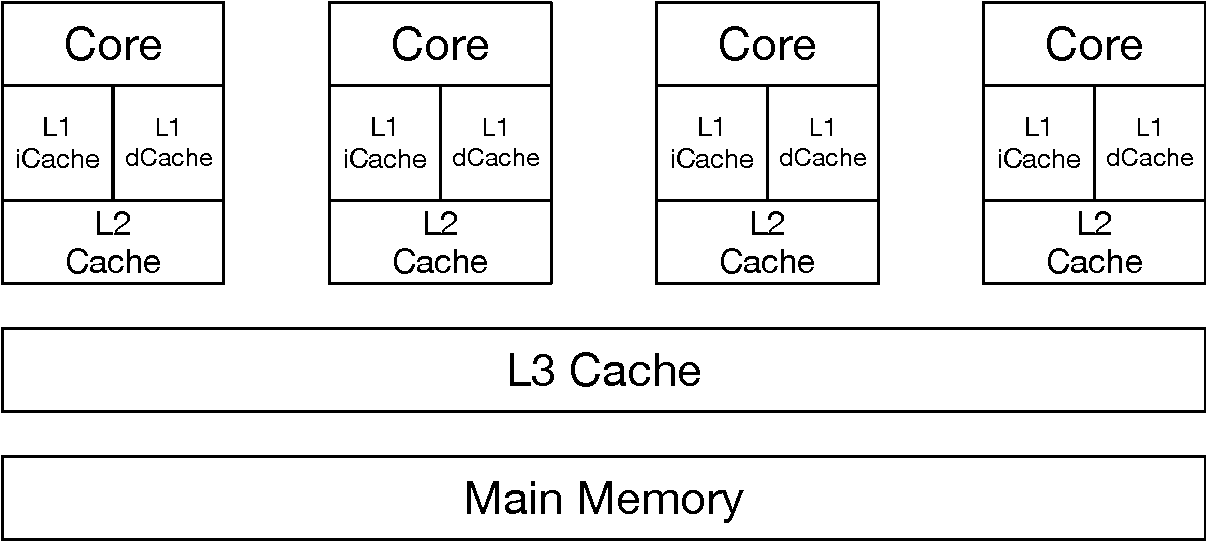
\includegraphics[width=.5\columnwidth]{./figures/chapter3/architecture.pdf}
  \caption{Computer memory hierarchy. The hierarchy is designed to minimise the access time with the relatively low cost. It is the root cause of many side-channel attacks.}\label{fig:memory_hierarchy}
\end{figure}

The current computer memory hierarchy opens the way for side-channel attacks from two aspects. First, the architecture relies on the system software to manage the memory, which becomes a problem in a threat model when the operating system is not untrusted (e.g., Intel SGX). Second, the size of the cache is smaller than the main memory. It is possible that different units in the main memory share the same address in the cache.
\begin{figure}[ht]
  \centering
  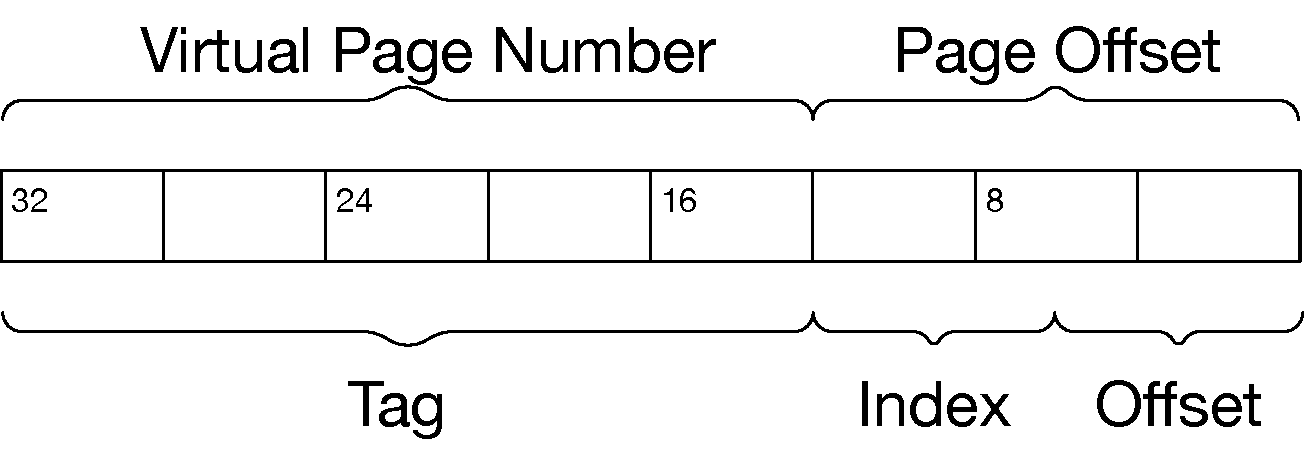
\includegraphics[width=.65\columnwidth]{./figures/chapter3/address.pdf}
  \caption{Memory addressing}\label{fig:memory_address}
\end{figure}

In modern CPUs, L1 and L2 caches are traditional N-way set associate caches. That is, the cache is divided into several cache sets, and each set contains several cache lines. The cache line is the atomic unit. As shown in Figure~\ref{fig:memory_address}, we can determine whether the data is in the cache with the following steps.  Given an address, the CPU uses the \textsf{Index} field of the address to locate the cache set that the address should reside in. After that, it tries to use the \textsf{Tag} field to match every cache line inside the set line. If the CPU can locate a cache line with the same tag and the valid bit is set, then a cache hit occurs. The CPUs use a similar process to manage the main memory. The main memory is divided into many units called pages. As shown in Figure~\ref{fig:memory_address},
the translation process keeps the bottom bits same while using the top bits to map the Physical Page Numbers to Virtual Page Numbers. 

\subsection{Threat Model}
We assume that an attacker shares the same hardware platform with the victim.
The attacker attempts to retrieve sensitive information through address-based side-channel attacks. The attacker has no direct access to the victim's data, but he can probe the memory or cache at each program point. Here are a few examples.
\begin{enumerate}
  \item A host machine has several virtual machines (VMs). The victim runs the application inside one VM. An attacker can control one VM and probe the process running on the other VM.
  \item  In a shielding system~\cite{arnautov2016scone,schuster2015vc3}, a malicious operating system can extract sensitive information from protected user-level applications.
  \item A ring-3 application can probe some sensitive information inside the kernel.
\end{enumerate}

In reality, attackers may face many possible obstacles, such as the noisy observations of the memory or cache. However, for this project, we assume the attacker has noise-free observations as in previous work~\cite{203878,182946,Brotzman19Casym}. The threat model captures most address-based side-channel attacks and apply to the three attack models: 1) time-based attacks, 2) access-based attacks, 3) trace-based attacks. We only consider deterministic programs and assume an attacker has access to the source code or binary executable of the target program.

\section{Limitations of Current Side-channel Leakage Detection Tools}
In this section, we introduce two limitations of current side-channel leakage detection tools. The first is that some tools have some false positives or false negatives. The second is that current tools are not fast enough to analyze side-channel leakages in real-world software.


\subsection{Imprecision}
In this dissertation, we study two types of side-channel leakage code patterns. The intuition is that the target application shows different control flows or data flows when it processes different sensitive input data. We refer them as \textit{secret-dependent control flow transfers} and \textit{secret-dependent data accesses}. Unlike previous work, our tool works on the machine code, which is more precise than previous tools that work on the source code or the intermediate representation.
\subsubsection{Control Flow}
\begin{figure}[ht]
  \begin{minipage}{0.45\linewidth}
    \begin{lstlisting}[xleftmargin=.15\textwidth, xrightmargin=.0\textwidth, frame=none]
int example1(uint8_t k, uint32_t m) { // m = 0
  uint32_t b = (k & m) >> 7;
  if (b) {
    ...    // Branch 1
  } else {
    ...    // Branch 2
  }
  ...
}
\end{lstlisting}
  \end{minipage}
  \hfill
  \begin{minipage}{0.45\linewidth}
    \begin{lstlisting}[xleftmargin=.15\textwidth, xrightmargin=.00\textwidth, frame=none, numbers=none, mathescape=true]
push  ebp
mov   ebp, esp
movzx eax, [addr_k]    
and   eax, [addr_me] 
shr   eax, 0x7           
test  eax, eax
jne   branch 2
...
\end{lstlisting}
  \end{minipage}\caption*{(a) A False Negative}

  \begin{minipage}{0.45\linewidth}
    \begin{lstlisting}[xleftmargin=.15\textwidth, xrightmargin=.0\textwidth, frame=none]
int example2(uint16_t k) {
  int res;
  if (k > 8) {
    res = 0;
  } else {
    res = 1;
  }
  return res;
}
\end{lstlisting}
  \end{minipage}
  \hfill
  \begin{minipage}{0.45\linewidth}
    \begin{lstlisting}[xleftmargin=.15\textwidth, xrightmargin=.00\textwidth, frame=none, numbers=none, mathescape=true]
xor   eax, eax
cmp   [addr_k], 8
setbe al
xor   edx, edx
ret
\end{lstlisting}
  \end{minipage}\caption*{(b) A False Positive}
  \caption{Secret-dependent control-flow transfers}\label{fig:chapter3:cf}
\end{figure}

If the input-sensitive data can affect the victim program's control flow, then an attacker can infer the sensitive data by observing the control flow during the execution. Figure~\ref{fig:chapter3:cf}(a) shows such an example. The function takes a public value \textsf{m} and a secret \textsf{k} as the inputs. The code at line 2 ensures that the lower 7 bits of the value \textsf{k} do not affect the value \textsf{b}. However, depending on the value of \text{m}, the code snippet in Figure~\ref{fig:chapter3:cf}(a) may have a leakage site. If the eighth bit of \textsf{m} is 1, then an attacker can infer the eighth bit of \textsf{k} by observing the branch at line 4 or line 6. The right figure shows the corresponding machine code. It has a conditional jump instruction \textsf{jne}. The sensitive input \textsf{k} can affect the program counter (the rip register), which is the root cause of the side-channel leakages.

However, the if-else branch does not always indicate there is a potential leakage site. Figure~\ref{fig:chapter3:cf}(b) shows a different situation. While the sensitive input \textsf{k} can affect the if-else branch, the compiler removes the branch with a conditional set instruction.  The opposite situation is the same. For example, recent work tries to use bit masking to rewrite the program with control flows. However, for some situations~\cite{Coppens:2009:PMT:1607723.1608124}, compilers (e.g., GCC) optimize the code too much (from a security view) and remove the unnecessary copy by reintroducing conditional moves.
\subsubsection{Data Flow}
\begin{figure}[ht]
  \begin{minipage}{0.4\linewidth}
    \begin{lstlisting}[xleftmargin=.15\textwidth, xrightmargin=.0\textwidth, frame=none]
uint8_t T[128];
...
int example3(uint8_t k, uint32_t m){
  uint32_t index = m;
  index = index + k % 128;
  uint8_t t = T[index];
  ...
}
\end{lstlisting}
  \end{minipage}
  \hfill
  \begin{minipage}{0.4\linewidth}
    \begin{lstlisting}[xleftmargin=.15\textwidth, xrightmargin=.00\textwidth, frame=none, numbers=none, mathescape=true]
...
lea    edx, [addr_T]
mov    eax, [addr_k]
and    eax, 0x7f
add    eax, [addr_m]
movzx  eax, [addr_T + eax*1]
...
\end{lstlisting}
  \end{minipage}\caption*{(a) A True Leakage}

  \begin{minipage}{0.4\linewidth}
    \begin{lstlisting}[xleftmargin=.15\textwidth, xrightmargin=.0\textwidth, frame=none]
uint8_t T[32];
...
int example4(uint8_t k, uint32_t m){
  uint32_t index = m;
  index = index + k % 32;
  uint8_t t = T[index];
  ...
}
\end{lstlisting}
  \end{minipage}
  \hfill
  \begin{minipage}{0.4\linewidth}
    \begin{lstlisting}[xleftmargin=.15\textwidth, xrightmargin=.00\textwidth, frame=none, numbers=none, mathescape=true]
...
lea    edx, [addr_T]
mov    eax, [addr_k]
and    eax, 0x3f
add    eax, [addr_m]
movzx  eax, [addr_T + eax*1]
...
\end{lstlisting}
  \end{minipage}\caption*{(b) A False Positive}
  \caption{Secret-dependent data accesses}\label{fig:chapter3:da}
\end{figure}

Figure~\ref{fig:chapter3:da} shows an example of the secret-dependent data access. \textsf{T} is an array with 128 elements. The size of each element is one byte. So the total size of the array is 128 bytes. Suppose an attacker can observe the memory access at the granularity of one cache lines (64 Bytes), then it is not possible to hold all the data inside the one cache line. An attacker can get some information of the value \textsf{secret} in Figure~\ref{fig:chapter3:da}(a) by observing the cache line access. Figure~\ref{fig:chapter3:da}(b) shows a different example. In this example, only 32 different elements can be accessed in the array and the size of the array is 32 bytes, which is smaller than the size of a cache line. Depending on the base address of the array, the array can be stored in one cache line or two consecutive cache lines. Therefore, such a code may still be vulnerable to side-channel vulnerabilities. However, existing tools (e.g., CacheD) use a concrete base address. Under the circumstance, these tools may miss such vulnerabilities.

\subsection{Performance}
The second limitation of current side-channel detection tools is the performance bottleneck, especially for tools based on symbolic analysis. For example, CaSym can only analyze small programs. CacheD performs better than CaSym. However, it still can not handle large programs such as RSA directly. It uses some domain knowledge to analyze only part of the program. The expensive cost comes from the symbolic execution. Symbolic execution can be used to explore all the possible paths, which is useful for many tasks.
Nevertheless, it is significantly less likely for cache side-channel bugs in crypto primitives. Cryptography primitives are more likely to have an even coverage of different paths (based on pseudo-random cipher states), and a branch-based side-channel is vulnerable from the very first branch on secret data, making complex path conditions less often relevant. Therefore, we choose to analyze a trace instead of the whole path. Another bottleneck is that the IR. While the IR can significantly decrease the difficulty of the implementation, it also gives introduce an average of 10x of the overall overhead. Third, using SMT solving can be convenient because of its generality, and it is commonly used for its precision when checking branch feasibility in symbolic execution. But the decision problems that an SMT solver handles are typically at least NP-hard. On the other hand, we can use some methods to avoid the solver and find side-channel leakages more efficiently.

\section{Method}\label{chapter3:method}
\begin{figure}[ht]
  \centering
  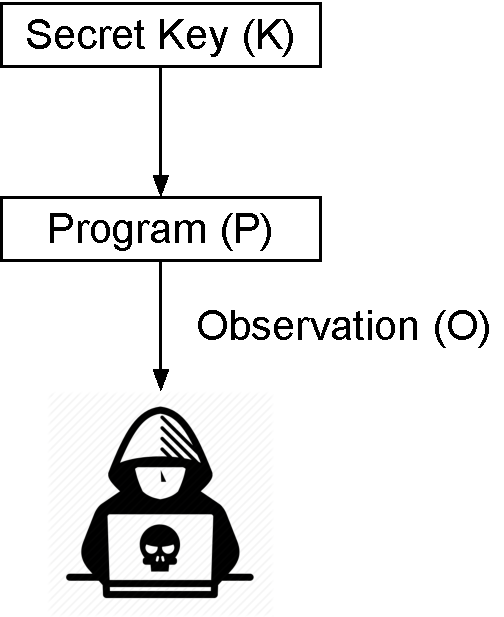
\includegraphics[width=.3\columnwidth]{./figures/chapter3/attack.pdf}
  \caption{A side-channel attack}\label{fig:side-channel-attack}
\end{figure}

In the section, we give necessary definitions and notations for dealing with
programs and side-channels.

Shown in Figure~\ref{fig:side-channel-attack}, a side-channel attack can be formulated into the following steps.  A program ($\beta$) has $K$ as its sensitive input (e.g., the encryption key) and $M$ as its the public input (e.g., the plaintext). In a real execution, an adversary may have
some observations ($O$) of the program. Examples of these observations include the timing, CPU usages, and electromagnetic signals (EM). In this dissertation, we use secret-dependent control flows and secret-dependent data
accesses as observations.

With the above definition, we have the following mapping between $\beta$, $K$, $M$, and $O$:
\begin{displaymath}
  \beta(K, M) \rightarrow O
\end{displaymath}


We model a side-channel in the following way. An adversary does not have
access to $K$, but he knows $\beta$, $M$, and $O$. For one execution of a
deterministic program, once $k \in K$ and $m \in M$ are fixed, the observation
($o \in O$) should also be determined. An attacker knows $\beta$, $o$,
and $m$. The attacker wants to infer the value of $k$. Moreover, we assume
an attacker can change the public input ($m \in M$) while keeping the secret input $k$. The threat model is similar to a chosen-plaintext attack.
We now discuss how to model observations ($O$),
which are the direct information that an adversary gets during the attack.

For one execution, a program ($\beta$) has many temporary values ($t_i \in
  T$). Once $\beta$ (program), $k$ (secret), and $m$ (message, public) are
determined, $t_i$ is also fixed. Therefore, $ t_i = f_i(\beta, k, m)$, where $f_
  i$ is a function that maps between $t_i$ and ($\beta$, $k$, $m$). In the chapter,
we consider two code patterns that can be exploited by an attacker,
\emph{secret-dependent control transfers} and \emph{secret-dependent data
  accesses}. 

\subsection{Secret-dependent Control Transfers}
A control-flow path is secret-dependent if different input-sensitive keys
($K$) can lead to different branch conditions.
We define a branch to be secret-dependent if:
$$\exists k_{i1}, k_{i2} \in K, m \in M, \,f_i(\beta, k_{i1}, m) \neq f_i(\beta, k_{i2}, m) \land PC$$

$PC$ represents the path condition. An adversary can observe which branch the code executes if the branch condition
equals $t_b$. We use the constraint $c_i : f_i(\beta, k, m) = t_b$ to model
the observation ($o$) on secret-dependent control-transfers. Note that in the
above definition, $m$ is also a variable. So it is possible for some $m \in M$,
we can not find a pair of two different $k_{i1}$ and $k_{i2}$ to satisfy the above inequation. For example, in Figure~\ref{fig:chapter3:cf}, if $m = \mathtt{0}$, the function \textsf{example1} will always execute the branch 2. However, if $m = \mathtt{0xffffffff}$ and $k = \mathtt{0}$, the function \textsf{example1} executes the branch 1 and the function \textsf{example1} executes the branch 2 when $k = \mathtt{0xf000000}$.


\subsection{Secret-dependent Data Accesses}
Similar to secret-dependent control-flow transfers, a data access operation is
secret-dependent if different input sensitive keys ($K$) cause access to different memory addresses. We use the model from CacheD~\cite{203878}. The low $L$ bits of the address are generally unimportant in side-channels.

A data access is secret-dependent if:

$$\exists k_{i1}, k_{i2} \in K, m \in M,\,f_i(\beta, k_{i1}, m) >> L \neq f_i(\beta, k_{i2}, m) >> L \land PC$$

If the memory access equals to $t_b$, we can use the constraint $c_i :
  f_i(\beta, k, m) >> L = t_b >> L$ to model the observation on secret-dependent
data accesses. Let's take a look the examples in Figure~\ref{fig:chapter3:da}(a).
Suppose the base address of the array \textsf{T} is 10. We symbolize both the $k$ and $m$. The formula that represents the memory access at line 6 is $10 + m + (k \mod 128)$. Therefore, we have the formula: $(10 + m + (k_1 \mod 128)) >> 6  \neq (10 + m + (k_2 \mod 128)) >> 6$.
Here is one possible solution: $m = 0, k_1 = 0, k_2 = 127$. In fact, for any $m$, we can always find possible $k_1$ and $k_2$ that satisfy the above inequation. It is a true leakage. The leakage can also be identified by previous tools such as CacheD. Similarly, we can model the memory access at line 6 with the formula:  $10 + m + (k_1 \mod 32) >> 6  \neq 10 + m + (k_2 \mod 32) >> 6$. If $m = 0$, we can not find satisfiable $k_1$ and $k_2$ for the above inequation, which indicates that it will always access the same cache line at line 6. However, it is possible that for some $m \in M$, we can find such a pair of $k_1$ and $k_2$ ($m = 53, k_1 = 1, k_2 = 0$). If the actual public input is $0$, existing tools (e.g., CacheD) can miss such a vulnerability. On the other hand, our tool can identify the leakages precisely.

\section{Scalability}
\subsection{Trace-oriented Symbolic Execution}
Symbolic execution is notorious for its expensive performance cost.
Previous trace-oriented symbolic execution
work~\cite{203878,Chattopadhyay:2017:QIL:3127041.3127044} has serious
performance bottlenecks. As a result, these approaches either apply only to
small programs~\cite{Chattopadhyay:2017:QIL:3127041.3127044} or require
domain knowledge~\cite{Wang:2007:NCD:1250662.1250723} to simplify the analysis.
These tools interpret each
instruction and update memory cells and registers with formulas that
captured the semantics of the execution and search different input values that
can lead to different execution behaviors using a constraint solver.
We implement the approach presented in \S\ref{chapter3:method} and model the side-channels as formulas. While the tools can analyze some simple cases such as AES, it cannot handle complicated examples such as RSA.
We observe that finding side-channels using symbolic execution differs from
traditional symbolic execution, and it can be optimized to be as efficient
as other methods.

\subsection{Interpret Instructions Symbolically}
Existing binary analysis frameworks~\cite{shoshitaishvili2016state,
  10.1007/978-3-642-22110-1_37, song2008bitblaze} translate machine instructions into
intermediate languages (IR) to simplify analysis since
the variety of machine instructions is
enormous, and their semantics is complex. The Intel Developer
Manual~\cite{intelsys} documents more than 1000 different x86 instructions.
Unfortunately, the IR layer, which
reduces the workload of these tools, is not suitable for side-channels
analysis because
IR-based or source code side-channels analyses do not represent the executed instructions accurate enough to analyze fully their control and memory accesses.
For example, a compiler may use conditional moves or bitwise operations to eliminate
branches. Also, as some IRs are not a superset or a subset of ISA,
it is hard to rule out conditional jumps introduced by IR and add real branches
eliminated by IR transformations.

Moreover, the IR causes significant overhead~\cite{217563}.
Translating machine instructions into IR is time-consuming. For example,
REIL IR~\cite{dullien2009reil}, adopted in CacheS~\cite{236338}, has multiple
transform processes, from binary to VEX IR, BAP IR, and finally REIL IR\@.
Also, IR increases the total number of instructions. For example, x86
instruction \textit{test eax, eax} transfers into 18 REIL IR instructions.

\textbf{Our Solution:}
We abandoned IR and expended the effort to implement
symbolic execution directly on x86 instructions.
Table~\ref{scala:ir} shows that eliminating the IR reduces the number
of instructions examined during analysis. Previous works~\cite{217563} also
adopted a similar approach to speed up fuzzing. Our implementation differs
from that work in two aspects: 1) We use complete constraints. 2) We run the
symbolic execution on one execution path each time. Our approach is approximately 30 times faster than using an IR (transferring ISA into IR and
symbolically executing it).

\begin{table}[ht]
  \centering\small\footnotesize
  \caption{The number of x86,  % instructions and the number of 
    REIL IR, and VEX IR instructions on the traces of crypto programs.}
  \label{scala:ir}
  \resizebox{.8\columnwidth}{!}{%

    \begin{tabular}{cccc}
      \hline
                        & \begin{tabular}[c]{@{}c@{}}Number of\\ x86 Instructions\end{tabular} & \begin{tabular}[c]{@{}c@{}}Number of\\ VEX IR\end{tabular} & \begin{tabular}[c]{@{}c@{}}Number of\\ REIL IR\end{tabular} \\ \hline
      AES OpenSSL 0.9.7 & $1,704$                    & $23,938$ (15x)             & $62,045$ (36x)             \\
      DES OpenSSL 0.9.7 & $2,976$                    & $41,897$ (15x)             & $100,365$ (33x)            \\
      RSA OpenSSL 0.9.7 & $1.6*10^7$                 & $2.4*10^8$ (15x)           & $5.9*10^8$ (37x)           \\
      RSA mbedTLS 2.5   & $2.2*10^7$                 & $3.1*10^8$ (15x)           & $8.6*10^8$  (39x)          \\ \hline
    \end{tabular}
  }
\end{table}

\subsection{Constraint Solving}
As discussed in the previous section, the problem of identifying
side-channels can be reduced to the question below.

\begin{quote}
  \textit{Can we find two different input variables $k_1, k_2 \in K$ that
    satisfy the formula $f_a(k_1) \neq f_a(k_2)$?}
\end{quote}

Existing approaches rely on satisfiability modulo theories (SMT) solvers
(e.g., Z3~\cite{DeMoura:2008:ZES:1792734.1792766}) to find satisfying assignments to
$k_1$ and $k_2$.
While this is a universal approach to solving constraints,
for constraints of this form, using custom
heuristics and testing is much more efficient in practice. Constraint
solving is a decision problem expressed in logic formulas. SMT solvers
transfer the SMT formula into the boolean conjunctive normal
form (CNF) and feed it into the internal boolean satisfiability
problem (SAT) solver. The translation process, called ``bit blasting'',
is time-consuming. Also, as the SAT problem is a well-known NP-complete
problem, it is hard to deal when it comes to
practical uses with huge formulas. Despite the rapid improvement
in SMT solvers in recent years, constraint solving remains one of
the obstacles to scaling the analysis of real-world crypto-systems.

\textbf{Our Solution:}
Instead of feeding the formula $f_a(k_1) \neq f_a(k_2)$ into a SMT solver, we
randomly pick $k_1, k_2 \in K$ and test them if they satisfy the
formula. Our solution is based on the following intuition. For most combination
of $(k_{1}, k_{2} )$, $f_a(k_1) \neq f_a(k_2)$. As long as
$f_a$ is not a constant function, such $k_1, k_2$ must exist. For example,
suppose each time we only have 5\% chance to find such $k_1, k_2$, then after we
test with different input combination with 100 times, we have $1 -
  (1-0.05)^{100} = 99.6\%$ chance find such $k_1, k_2$. This type of random algorithm works well for our problem.

\section{Design and Implementation}
\subsection{Trace Logging}
The trace information can be logged via some emulators (e.g., QEMU) or dynamic binary instrumentation tools (DBI).
In this work, we run a program with the concrete input under the DBI to record execution traces.
The trace data has the following information:
\begin{itemize}
  \item Each instruction mnemonics and its memory address.
  \item The operands of each instruction and their concrete values during the runtime.
  \item The value of EFLAGS register.
  \item The memory address and the length of the sensitive information.
        Most crypto libraries stores sensitive information in arrays,
        variables or contiguous buffer.
\end{itemize}

\subsection{Instruction Level Symbolic Execution}
\label{InstructionSE}
The primary purpose of the step is to generate constraints of the input sensitive information from the execution trace. If we give the target program a new input which is different from the original input that was used to generate the execution trace but still satisfies these constraints, as an attacker, he will have the same observations on control-flow transfers and data-access patterns.

The tool runs symbolic execution on top of execution traces. At the beginning of the symbolic execution, the tool creates new symbols for each byte in the raw buffer. For other data in the register or memory at the beginning, we use actual values from the runtime information collected during the runtime. During the symbolic execution for each instruction, the tool updates every variable in the memory and registers with a math formula. The formula is made up of concrete values and the input key as the symbols accumulated through the symbolic execution. We implement several rules to simplify the formulas. For each formula, the tool will check weather it can be reduced into a concrete values (e.g., $k_1+12-k_1 = 12$ ). If so, the tool will only use the concrete values in the following symbolic execution.

\subsubsection{Verification and Optimization}
We run the symbolic execution (SE) on top of x86 instructions. In other words, we do not rely on any intermediate languages to simplify the implementation of symbolic execution. While the implementation itself has a lot of benefits (Better performance, accurate memory model), we need to implement the symbolic execution rules for each x86 instruction.
However, due to the complexity of x86, it is inevitable to make mistakes. Therefore, we verify the correctness of the SE engine during the execution.
The tool will collect the runtime information (Register values, memory values) and compare them with the formula generated from the symbolic execution. Whenever the tool finishes the symbolic execution of each instruction, the tool will compare the formula for each symbol and its actual value. If the two values do not match, we check the code and fix the error. Also, if the formula does not contain any symbols, the tool will use the concrete value instead of symbolic execution.

\subsubsection{Secret-dependent Control-flows}
An adversary can infer sensitive information from secret dependent control-flows. There are two kinds of control-transfer instructions: the unconditional control-transfer instructions and the conditional transfer instructions.
The unconditional instructions, such as CALL, JUMP, RET transfer control from one code segment location to another. Since the transfer is independent of the input sensitive information, an attacker was not able to infer any sensitive information from the control-flow.
So the unconditional control-transfer does not leak any information based on our threat model. During the symbolic execution, we update the register information and memory cells with new formulas accordingly.

The conditional control-flow transfer instructions, such as conditional jumps, depending on CPU states, may or may not transfer control flows. For conditional jumps, the CPU will test if certain condition flag
(e.g., CF = 0, ZF =1) is met and jump to certain branches, respectively.
The symbolic engine will compute the flag and represent the flag in a symbol
formula. Because we are running on a symbolic execution on an execution trace, we know which branch is executed.
If a conditional jump uses the CPU status flag, we will generate the constraint accordingly.

For examples, considering the below x86 code snippet,

\begin{lstlisting}[xleftmargin=.3\textwidth, xrightmargin=.2\textwidth, frame=none][ht]
...
0x0000e781      add dword [local_14h], 1
0x0000e785      cmp dword [local_14h], 4
0x0000e789      jne 0xe7df
0x0000e78b      mov dword [local_14h], 0
...
\end{lstlisting}

At the address $\mathtt{0x0000e781}$, the value at the address of $\mathtt{local\_14h}$ can be written as $F(\vec{K})$. At the address $\mathtt{0x0000e785}$, the value will be updated with $F(\vec{K})+1$. Then the code compares the value with $4$ and use the result as a conditional jump. Based on the result, we can have the following formula:

$$F(\vec{K}) + 1 = 4$$

The formula, together with the memory address ($\mathtt{0x0000e789}$) is stored as a \textit{formula tuple (address, formula)}. Each formula tuple represents one potential leakage site.

\subsubsection{Secret-dependent Data Accesses}
Like input-dependent control-flow transfers, an adversary can also infer sensitive information from the data access pattern as well. We try to find this kind of leakages by checking every memory operand of the instruction. We generate the memory addressing
formulas. As discussed before, every symbols in the formula is the input key. If the formula does not contain any symbols, the memory access is independent
from the input sensitive information and will not leak any sensitive information according to our threat model. Otherwise, we will generate the constraint for
the memory addressing. We model the memory address with a symbolic formula $F(\vec{K})$. Because we also have the concrete value of the memory address $\mathtt{Addr1}$. Inspired by the work from~\cite{203878}, the formula can be written as:

$$F(\vec{K}) >> L = \mathtt{Addr1} >> L$$

$L$ represents the minimum memory address granularity that an attacker can observe. For example, Flush and Reload can distinguish between different cache lines, which means the value of L is 6.

\subsubsection{Information Flow Check}
\detect{} is designed to help software developers find and understand the side-channel vulnerabilities. To ease the procedure of fixing bugs, we also track the information flow for each byte of the input
buffer.
The step can be seen as the multiple-tag taint analysis. With the help of the information from symbolic execution, we can implement a relatively simple but relatively precise information flow track.
At the beginning of the analysis, \detect{} keep track of each byte in
the original buffer. When \detect{} symbolically executes each instruction in the trace, it will check every value read from registers or memory. If the value is concrete, it means the instruction has nothing to do with the original buffer.
If the value is a formula, it means the original information passes through the instruction. Since each byte in the sensitive buffer is represented as a symbol with a unique ID, \detect{} can know which byte in the origin buffer goes through the instruction.

\section{Evaluation}
We evaluate our method on real-world crypto libraries, which include  OpenSSL, mbedTLS, Libgcrypt and Monocypher\@. OpenSSL is the most commonly used crypto libraries in today's software. mbedTLS\@ (previous known as PolarSSL) is designed to be easy to understand and fit on embedded devices. We also evaluate Monocypher, a new cryptographic library that resists to most side-channel attacks.
According to the developers, Monocypher is designed to have no secret dependent indices and secret dependent branches. Therefore, Monocypher should be secure under our threat model. Libgcrypt is a cryptographic library from the GunPG. As some previous work (e.g., CacheD) choose to evaluate their tools on Libgcrypt, we can compare the evaluation results by applying the tool on Libgcrypt.

For some crypto libraries, we evaluate multiple versions. After that, we compare the evaluation results with the version history to track these leakages' patches. In summary, we evaluate our tool on the following libraries.
\begin{itemize}
  \item OpenSSL: 0.9.7, 1.0.2f, 1.0.2k, 1.1.0f, 1.1.1, 1.1.1g
  \item MbedTLS: 2.5, 2.15
  \item Libgcrypt: 1.6.1, 1.7.3, 1.8.5
  \item Monocyper: 3.0
\end{itemize}

We refer to the examples or test cases of these libraries and write simple
programs that use the crypto libraries. For symmetric encryption, the length
of the keys are 256 bit. For RSA, the length of the keys is 1024. For ECDSA, the
length of the key is 384 bit. The input public message is ``Hello World!''.
We mark variables and buffers that store a secret.
For DES and AES, we mark symmetric keys as secrets.
For RSA, we mark private keys as secrets. For ECDSA,
we mark nonces and private keys as secrets.

We build the source program into 32-bit x86 Linux executables with GCC 7.5
running on Ubuntu 16.04. While our tool can work on the stripped binaries, 
in the evaluation, we keep the debug information to get the fine-grained information
(e.g., line numbers).
We run our experiments on a 2.90GHz Intel Xeon(R) E5-2690 CPU with 128GB
RAM. We run the experiments simultaneously, but the execution time is calculated on a single-core.

During our evaluation process, we are interested in the following
aspects:
\begin{enumerate}
    \item Is \detect{} effective to detect side-channels in real-world crypto systems? (Effectiveness)
    \item How much performance overhead does the method introduce? (Performance)
\end{enumerate}

\subsection{Evaluation Result Overview}
\begin{table*}
  \centering\small\footnotesize
  \caption{Evaluation results overview: Algorithm, Implementation, Side-channel Leaks\,(Leaks),
    Secret-dependent Control-flows\,(CF), Secret-dependent Data-flows\,(DF),
    The number of instructions\,(\# Instructions), The Execution Time, and The Memory Usage.
  }\label{table:over_result}
  \begin{tabular}{llrrrrrr}
    \hline
    \textbf{Algorithm} & \textbf{Implementation}  & \textbf{\# Leaks} & \textbf{\# CF}    & \textbf{\# DF}
                       & \textbf{\# Instructions} & \textbf{Time}     & \textbf{RAM (MB)}                                                  \\\hline
                       &                          &                   &                   &                &             & ms              \\\cline{7-7}
    AES                & mbedTLS 2.5              & 68                & 0                 & 68             & 39,855      & 512     & 47    \\
    AES                & mbedTLS 2.15             & 68                & 0                 & 68             & 39,855      & 520     & 47    \\
    AES                & OpenSSL 0.9.7            & 75                & 0                 & 75             & 1,704       & 231     & 15    \\
    AES                & OpenSSL 1.0.2f           & 88                & 0                 & 88             & 1,350       & 36      & 15    \\
    AES                & OpenSSL 1.0.2k           & 88                & 0                 & 88             & 1,350       & 35      & 16    \\
    AES                & OpenSSL 1.1.0f           & 88                & 0                 & 88             & 1,420       & 36      & 16    \\
    AES                & OpenSSL 1.1.1            & 88                & 0                 & 88             & 1,586       & 43      & 16    \\
    DES                & mbedTLS 2.5              & 15                & 0                 & 15             & 4,596       & 58      & 8     \\
    DES                & mbedTLS 2.15             & 15                & 0                 & 15             & 4,596       & 57      & 8     \\
    DES                & OpenSSL 0.9.7            & 6                 & 0                 & 6              & 2,976       & 163     & 11    \\
    DES                & OpenSSL 1.0.2f           & 8                 & 0                 & 8              & 2,593       & 166     & 11    \\
    DES                & OpenSSL 1.0.2k           & 8                 & 0                 & 8              & 2,593       & 165     & 11    \\
    DES                & OpenSSL 1.1.0f           & 8                 & 0                 & 8              & 4,260       & 182     & 21    \\
    Triple DES         & OpenSSL 1.1.0f &  9 &0  &9   &13,105   & 369 & 56\\
    DES                & OpenSSL 1.1.1            & 6                 & 0                 & 6              & 8,272       & 229     & 43    \\
                       &                          &                   &                   &                &             & seconds         \\\cline{7-7}
    Chacha20           & Monocypher 3.0           & 0                 & 0                 & 0              & 149,353     & 2       & 15    \\
    Poly1305           & Monocypher 3.0           & 0                 & 0                 & 0              & 1,213,937   & 15      & 43    \\
    Argon2i            & Monocypher 3.0           & 0                 & 0                 & 0              & 4,595,142   & 37      & 102   \\
    Ed25519            & Monocypher 3.0           & 0                 & 0                 & 0              & 5,713,619   & 271     & 98    \\
    ECDSA              & mbedTLS 2.5              & 6                 & 6                 & 0              & 4,214,946   & 48      & 689   \\
    ECDSA              & mbedTLS 2.15             & 4                 & 4                 & 0              & 4,192,558   & 102     & 680   \\
    ECDSA              & OpenSSL 1.0.2f           & 5                 & 4                 & 1              & 8,248,322   & 101     & 980   \\
    ECDSA              & OpenSSL 1.0.2k           & 5                 & 4                 & 1              & 8,263,599   & 100     & 906   \\
    ECDSA              & OpenSSL 1.1.0f           & 5                 & 4                 & 1              & 6,100,465   & 76      & 705   \\
    ECDSA              & OpenSSL 1.1.1            & 0                 & 0                 & 0              & 10,244,076  & 121     & 1,048 \\
    ECDSA              & OpenSSL 1.1.1g           & 0                 & 0                 & 0              & 9,266,191   & 102     & 1,001 \\

                       &                          &                   &                   &                &             & minutes         \\\cline{7-7}
    RSA                & mbedTLS 2.5              & 6                 & 6                 & 0              & 22,109,246  & 39      & 3,708 \\
    RSA                & mbedTLS 2.15             & 12                & 12                & 0              & 24,484,441  & 44      & 4,012 \\
    RSA                & OpenSSL 0.9.7            & 107               & 105               & 2              & 17,002,523  & 23      & 3,601 \\
    RSA                & OpenSSL 1.0.2f           & 38                & 27                & 11             & 14,468,307  & 29      & 3,301 \\
    RSA                & OpenSSL 1.0.2k           & 36                & 27                & 9              & 15,285,210  & 40      & 3,402 \\
    RSA                & OpenSSL 1.1.0f           & 31                & 22                & 9              & 16,390,750  & 34      & 3,701 \\
    RSA                & OpenSSL 1.1.1            & 4                 & 4                 & 0              & 18,207,016  & 8       & 4,181 \\
    RSA                & OpenSSL 1.1.1g           & 8                 & 8                 & 0              & 18,536,796  & 5       & 3,901 \\
    RSA                & Libgcrypt 1.6.1          & 11                & 9                 & 2              & 9,527,231   & 2       & 2516  \\
    RSA                & Libgcrypt 1.7.3          & 14                & 14                & 0              & 10,513,606  & 14      & 2,701 \\
    RSA                & Libgcrypt 1.8.5          & 8                 & 8                 & 0              & 27,407,986  & 113     & 4,701 \\

    Total              &                          & 913               & 241               & 672            & 167,155,052 & 341m            \\\hline
  \end{tabular}
\end{table*}
Table~\ref{table:over_result} summarizes the results.
\detect{} finds 913 leaks in the crypto libraries.
Among these 913 leaks, 241 are due to secret-dependent
control-flow transfers and 672 are due to secret-dependent data accesses.

The evaluated algorithms can be classified into two categories: symmetric
encryption and asymmetric encryption. Most of the side-channel leakages in symmetric implementations are from the lookup tables. The new implementation of OpenSSL has adopted several methods (e.g., one single S-box instead of four lookup tables, smaller lookup tables) to mitigate the problem. 

We also evaluate our tool on the RSA implementation. With the optimization
introduced in the previous sections, we need not apply domain knowledge to
simplify the analysis. Our tool identifies all leakage sites
reported by CacheD~\cite{203878} and find new leaks in less time.
We also find newer versions of RSA in OpenSSL have fewer leaks. Our tool can
finish all the analysis in less than 6 hours. 

\subsection{Comparison with the Existing Tools}
\label{eval:scala}

In this section, we compare \detect{} with the
existing trace-based side-channel detection tools on vulnerability detections. For other tools, we use the reported results in their papers. As other tools do not quantify leakage sites, we only include the time of detecting vulnerabilities to perform a fair comparison.

The comparison result with CacheD~\cite{203878} is shown in Table~\ref{eval:cacheD}.
Note that one statement in the source code can be compiled into several machine instructions. So it is possible that one statement can have multiple leakage points. Under the circumstance, we think it is only a leakage.
We have confirmed that \detect{} can identify all the secret-dependent data access vulnerabilities reported by CacheD. In addition, \detect{} finds many new ones.
CacheD fails to detect some vulnerabilities for two
reasons. First, CacheD can only detect secret-dependent data access
vulnerabilities. \detect{} can detect secret-dependent control-flows as well.
Second, according to the CacheD paper, CacheD times out after 20 hours to process
asymmetric ciphers. CacheD applies some domain knowledge to simplify and speed up
the analysis.
While these optimizations do not introduce false positives, they may miss some
vulnerabilities.
Third, CacheD only symbolizes the encryption keys. Some side-channel leakages when the input messages equal to some certain values. It is possible that CacheD miss some
leakages as we have discussion the previous sections.
We notice that the number of instructions in these traces are different due to the different analysis starting functions and building options during the evaluation.
Table~\ref{eval:cacheD} shows that
\detect{} is faster than CacheD. \detect{} is much faster than CacheD when analyzing the same
number of instructions. For example, when we test~\detect{} on AES from OpenSSL
0.9.7, \detect{} is over 100x faster than CacheD.
\begin{table*}[ht]
 \centering
  \caption{Comparison with CacheD: Time,
    Secret-dependent Control-flows\,(CF), Secret-dependent Data-flows\,(DF), The Number of Instructions\,(\# Instructions).}
  \label{eval:cacheD}

    \begin{tabular}{@{}l|r@{~~}r@{~~}r|r@{~~}r@{~}r@{}}
      \hline
      \multicolumn{1}{l|}{} & \multicolumn{3}{c|}{CacheD} & \multicolumn{3}{c}{Abacus}                                             \\
      Benchmark                  & Time (s)                    & \# Instructions            & DF & Time (s) & \# Instructions & CF+DF   \\ \hline
      AES OpenSSL 0.9.7         & 43.4                        & 791                        & 48 & 0.23     & 1,704           & 0+75    \\
      AES OpenSSL 1.0.2f       & 48.5                        & 2,410                      & 32 & 0.04     & 1,350           & 0+88    \\
      RSA OpenSSL 0.9.7       & 199.3                       & 674,797                    & 1  & 1,351.6  & 17,002,523      & 105+2   \\
      RSA OpenSSL 1.0.2f     & 165.6                       & 473,392                    & 1  & 1,753.3  & 14,468,307      & 27+11   \\
      RSA Libgcrypt 1.6.1     & 11542.3                     & 26,848,103                 & 2  & 128.1    & 9,527,231       & 9+2     \\
      RSA Libgcrypt 1.7.3         & 10788.9                     & 27,775,053                 & 0  & 891.7    & 10,513,606      & 14+0    \\ \hline
      Total                 & 22,788.0                    & 55,738,546                 & 84 & 4,125.0  & 51,514,721      & 155+178 \\ \hline
      \multicolumn{7}{l}{\# of Instructions per second \qquad  CacheD: 2,445 \qquad \tool: 12,489}                                 \\ \hline
    \end{tabular}

\end{table*}

DATA~\cite{217537} identifies
side-channel leakages by finding differences in execution traces of
the test program under \emph{various secret inputs}. According to
the original DATA paper, it uses 443 different traces to analyze the
side-channel vulnerabilities in symmetric cyphers and 450 different
traces to analyze the side-channel vulnerabilities in asymmetric
cyphers. On the other hand, \detect{} detects side-channel
vulnerabilities from one execution trace. \detect{} uses symbolic
analysis to extract formulas that model each side-channel
leakage. After that, we sample the formula with \emph{various
  secret inputs} to detect and quantify each leakage site. In
theory, DATA might have better code coverage than \detect{} because it
uses more execution traces,  but \detect{} has the following
advantages. a) \detect{} is faster than DATA. For example, it takes
116 minutes for DATA to detect vulnerabilities in the RSA implementation in OpenSSL 1.1.0f\@. \detect{} only spends 34 minutes, as shown in Table~\ref{table:over_result}. It takes 13 minutes and 20 minutes
for DATA to analyze the side-channel leakages in AES and DES,
respectively. On the other hand, \detect{} finishes its analysis in
less than ten seconds while finding all the leakages reported by
DATA. b) Because \detect{} does not exexute the test program again when we
have a new \emph{secret input}, \detect{} can test more input secrets
on these formulas within the same time to achieve better precision.
c) DATA tries to use leakage models (domain knowledge) to classify each leakage.
The strength of \ctool{} is that it does not need such domain knowledge.
DATA reports 278 control-flow and 460 memory-access leaks for the RSA implementation in OpenSSL 1.1.0f. Among these leakages, they find one new vulnerability in RSA after some manual analysis.
\detect{} finds the vulnerability.  For each leakage site, \detect{} can provide
concrete examples to trigger the issue.
\subsection{Case Studies}
\subsubsection*{DES and AES}
Our tool confirms that both implementations in OpenSSL and mbedTLS have side-channel leakages
sites. Moreover, we find that all the leakages belong to the secret-dependent data accesses. The reference implementation of AES uses four lookup tables to speed up the computation. However, such implementation are vulnerable to side-channel attacks. Previous work has shown an end-to-end attack to fully recover the key. Our findings is similar to the previous work. We also notice that later version of OpenSSL (after 1.0.1) uses a modified version with smaller S-table. However, \detect{} also find the leakage sites in the version. Recent work also finds the sites through theoretical analysis.

\subsubsection*{RSA}
We also evaluates our tool on the RSA implementations. With the optimizations
introduced in the previous section, we do not apply any domain knowledge to
simplify the analysis. Therefore, our tools can identify all the leakage sites
reported by CacheD~\cite{203878} in a shorter time. Our tool finds that most
leakages in RSA occur in the big number implementation. We also find the newer
versions of RSA in OpenSSL tend to have fewer leakages detected by \detect{}. 

Even for the up-to-date version of OpenSSL, \detect{} still find several
side-channel leakages. Figure~\ref{chapter3:fig:unknown_leakage} shows an unknown leakage site in OpenSSL 1.1.1. It is a secret-dependent control flow transfers. 
However, as the branch is inside a loop and a bit shift function causes the branch leak different bits from the sensitive buffer.

\begin{figure}[ht]
\centering
\begin{lstlisting}[xleftmargin=.02\textwidth,xrightmargin=.01\textwidth]
while (!BN_is_bit_set(B, shift)) { /* note that 0 < B */
    shift++;
    if (BN_is_odd(X)) {
        if (!BN_uadd(X, X, n))
            goto err;
    }
    ...
    if (!BN_rshift1(X, X))  // It causes the leak severe!
        goto err;
    ...
}
\end{lstlisting}
    \caption{Unknown sensitive secret-dependent branch leaks from function 
             \textsf{int\_bn\_mod\_inverse} in OpenSSL 1.1.1. The function can leak the last digit from big number \textbf{X}. However, the leak is more severe because of the 
             function \textsf{BN\_rshift1}. Each time function \textsf{BN\_rshift1}
             will shift \textbf{X} right by one and places the result in \textbf{X}. Therefore,
             an attacker can infer multiple bits of \textbf{X} by observing the branch at line 3.}
    \label{chapter3:fig:unknown_leakage}
\end{figure}


\subsubsection*{Monocypher}\label{eval:mono}
Monocypher is a small, easy to use cryptographic library with
performance comparable to LibSodium~\cite{libsodium} and NaCl~\cite{bernstein2012security}.
We choose four ciphers that are
designed to be side-channel resistant from the library.
Because these ciphers have no
data flow from secrets to branch conditions and load addresses.
Monocypher should be safe under our threat models.
We analyze these ciphers with \detect{}, and it reports no leaks.
This indicates that \detect{} is effective for validating countermeasures.







% !TEX root = ../YourName-Dissertation.tex

\chapter{Precise Analysis on Single-trace Attacks}\label{chapter4}

\section{Problem}
In Chapter~\ref{chapter3}, we present a method to identify address-based side-channel leakage sites in cryptography libraries ~\cite{Osvik2006,Gullasch:2011:CGB:2006077.2006784,203878,10.1007/978-3-540-45238-6_6}. However, many reported leakage sites are not patched by the developers. Recent work on side-channel vulnerability identification~\cite{203878,217537,Wichelmann:2018:MFF:3274694.3274741,Brotzman19Casym,236338,182946} also faced the same situation. For example, DATA~\cite{217537} reports 2,248 potential leakage sites for the RSA implementation in OpenSSL 1.1.0f\@. Further analysis shows 1,510 leaks can be dismissed, but that still leaves 460 data-access leaks and 278 control-flow leaks. Many of these vulnerabilities have not been fixed by the developers for a variety of reasons.

First, some vulnerable implementations perform better. For example,
RSA implementations usually adopt the Chinese Remainder Theorem (CRT) optimization, which is faster but vulnerable to fault attacks~\cite{aumuller2002fault}. Second, fixing old vulnerabilities can introduce new
weaknesses. Third, most vulnerabilities pose a negligible risk. Although some vulnerabilities result in the key being entirely compromised~\cite{184415, aumuller2002fault}, many others are less severe in reality. Therefore, we need a proper quantification metric to assess the sensitivity of side-channel vulnerabilities, so a developer can efficiently triage them.

Previous work on side-channel quantification~\cite{182946,5207642} can identify numerous leakages or even provide an upper bound on the amount of leakage, which is useful to verify that an implementation is secure if it incurs zero leakage.
However, these techniques cannot quantify the severity of a leak because they over approximate the leakage. For example, CacheAudit~\cite{182946}
reports that the upper-bound leakage of AES-128 exceeds the original key size. Besides, existing side-channel quantification work~\cite{182946,5207642} assumes an attacker runs the target program multiple times with different
input secrets and calculates an ``average'' estimation, which is different from real attack scenarios when the secret that an attacker wants to retrieve is fixed. As a consequence, these results are less useful in assessing the severity level of each leakage site.

To overcome these limitations, we propose a novel method to quantify information
leakage precisely. We quantify the number of bits that can be leaked during a real
execution and define the amount of leaked information as the cardinality of
possible secrets based on an attacker's observation. Before an attack, an adversary has a large but finite input space.
Whenever the adversary observes a leakage site, he can eliminate some impossible
inputs and reduce the input space's size. In an extreme case, if the input space's size reduces to one, an adversary has determined the input, which means all secret information (e.g., the entire secret key) is
leaked. By counting the number of inputs~\cite{10.1007/11499107_24}, we can quantify the information leakage precisely.
We use symbolic execution to generate constraints to model the relation
between the original sensitive input and an attacker's observations.
Symbolic execution provides fine-grained information, but it is expensive
to compute. Therefore, prior symbolic
execution work~\cite{203878,236338,Brotzman19Casym} either analyzes only
small programs or applies domain knowledge~\cite{203878} to simplify the analysis. We
examine the bottleneck of the trace-oriented symbolic execution and optimize it
to work for real-world crypto-systems.

We have implemented the proposed technique in a tool called \tool{} and demonstrated
it on real-world crypto libraries, including OpenSSL,
mbedTLS, Libgcrypt, and Monocypher.
We collect execution traces of these libraries and apply
symbolic execution to each instruction. We model
each side-channel leak as a logic formula. These
formulas precisely model side-channel vulnerabilities.
Then we use the conjunction of these formulas to model the
leaks at a statement that appears in different location in
the execution trace file (e.g., leaks inside a loop).
Finally, we introduce a Monte Carlo sampling method to estimate
the information leakage.
The experimental results confirm
that \tool{} precisely identifies previously known vulnerabilities and
reports how much information is leaked and which byte in the original sensitive
buffer is leaked. We also test \tool{} on side-channel-free algorithms.
\tool{} produces no false positives.
The result also shows the newer version of crypto libraries leak less information
than earlier versions.
\tool{} also discovers new vulnerabilities. With the help of \tool{},
we confirm that some of these vulnerabilities are severe.


%Based on the fixed attack target, we classify the software-based side-channel
%vulnerabilities into two categories: 1.\textit{secret-dependent control-flow
%transfers} and 2.\textit{secret-dependent data accesses} and model them with
%math formulas which constrain the value of sensitive information. We quantify
%the amount of leaked information as the number of possible solutions that are
%reduced after applying each constrains.


%Our method can identify and quantify address-based sensitive information
%leakage sites in real-world applications automatically. Adversaries can exploit
%different control-flow transfers and data-access patterns when the program
%processes different sensitive data. We refer them as the potential information
%leakage sites. Our tool can discover and estimate those potential information
%leakage sites as well as how many bits they can leak. We are also able to
%report precisely how many bits can be leaked in total if an attacker observes
%more than one site. We run symbolic execution on execution traces. We model
%each side-channel leakage as a math formula. The sensitive input is divided
%into several independent bytes and each byte is regarded as a unique symbol.
%Those formulas can precisely model every the side-channel vulnerability. In
%other words, if the application has a different sensitive input but still
%satisfies the formula, the code can still leak the same information.  
%Those information leakage sites may spread in the whole program and their
%leakages may not be dependent. Simply adding them up can only get a coarse
%upper bound estimate. In order to accurately calculate the total information
%leakage, we must know the dependent relationships among those multiple leakages
%sites. Therefore, we introduce a monte carlo sampling method to estimate the
%total information leakage.

In summary, we make the following contributions:

\begin{itemize}
    \item We propose a novel method that can quantify fine-grained leaked
          information from side-channel vulnerabilities that result from actual attack
          scenarios. Our approach differs from previous ones in that we
          model real attack scenarios for one execution.
          We model the information quantification problem as a counting problem
          and use a Monte Carlo sampling method to estimate the information leakage.

    \item We implement the method into a tool and apply it
          to several pieces of real software. \tool{} successfully identifies
          previous unknown and known side-channel vulnerabilities and calculates the corresponding information leakage.
          Our results are useful in practice.
          The leakage estimates and the corresponding trigger inputs can
          help developers to triage and fix the vulnerabilities.
\end{itemize}

\section{Threat Model}

The threat model in this chapter is similar to the threat model in our previous work from Chapter~\ref{chapter3}. Prior work~\cite{203878,182946,Brotzman19Casym} also shares the same threat model. That is, we assume
an attacker can share some hardware resource with the victim. The attacker has
the ability to probe the victim at any time of the execution. We also assume
an attacker has noise-free observations. The attacker has the access to the victim's
binary executable.  We believe that the majority of address-based side-channel attacks in the literature applies to the thread model.


\section{Background}
Given an event $e$ that occurs with the probability $p(e)$, we receive
\begin{displaymath}
    I = - \log_2p(e)
\end{displaymath}
bits of information by knowing the event $e$ happens according to information theory~\cite{shannon1948mathematical}.
Considering a char variable $a$
with one byte storage size in a C program, its value ranges from 0 to 255.
Assume $a$ has a uniform distribution. If we observe that
$a$ equals $1$, the probability of this observation is $\frac{1}{256}$. So
we get $-\log(\frac{1}{256}) = 8$ bits information, which is exactly the size
of a char variable in the C program.

Existing work on information leakage quantification typically uses Shannon
entropy~\cite{clark2007static,Wichelmann:2018:MFF:3274694.3274741},
min-entropy~\cite{10.1007/978-3-642-00596-1_21}, and max-entropy~\cite{182946,
    Doychev:2017:RAS:3062341.3062388}. In these frameworks, the input sensitive
information $K$ is considered as a random variable.

Let $k$ be one of the possible
value of $K$. The Shannon entropy $H(K)$ is defined as
\begin{displaymath}
    H(K) = - \sum_{k {\in} K}p(k)\log_2(p(k)).
\end{displaymath}

Shannon entropy can be used to quantify the initial uncertainty about the
sensitive information. It measures the amount of information in a system.

Min-entropy describes the information leaks for a program with the most likely input.
For example, min-entropy can be used to describe the
best chance of success in guessing one's password using the
most common password. %, which is defined as
\begin{displaymath}
    \mathit{min\text{-}entropy} = - \log_2(p_{\mathit{max}})
\end{displaymath}

Max-entropy is defined solely on the number of possible observations.
%It is equal to $-\log_2{n}$.
\begin{displaymath}
    \mathit{max\text{-}entropy} = -\log_2{n}
\end{displaymath}
As it is easy to compute, most recent works~\cite{182946,Doychev:2017:RAS:3062341.3062388} use max-entropy as the definition of
the amount of leaked information.

To illustrate how these definitions work, we consider the code
fragment in Figure~\ref{fig:side-channel}. It has two secret-dependent
control-flows, A and B.

\begin{figure}[h!]
    \centering
    \begin{lstlisting}[xleftmargin=.1\textwidth, xrightmargin=.1\textwidth]
uint8_t key[2], t1, t2;
get_key(key);              // 0 <= key[0], key[1] < 256
t1 = key[0] + key[1];
t2 = key[0] - key[1];
if (t1 < 4){               // leakage site A
    foo();    
}                          
if (t2 > 0){               // leakage site B     
    doo();    
}                          
\end{lstlisting}
    \caption{Side-channel leakage}
    \label{fig:side-channel}
\end{figure}
In this chapter, we assume an attacker can observe the secret-dependent control-flows in Figure~\ref{fig:side-channel}.
Therefore, an attacker can have two different observations for each leak site
depending on the value of the $\mathit{key}$: $A$ for function \textsf{foo} is executed,
$\neg A$ for function \textsf{foo} is not executed, $B$ for function \textsf{doo} is
executed, and $\neg B$ for function \textsf{doo} is not executed. Now the
question is how much information can be leaked from the above code if an
attacker knows which branch is executed?

\begin{table}[ht]
    \centering%\small\footnotesize
    \caption{The distribution of observations}\label{shtable}
    %    \resizebox{\columnwidth}{!}{
    \begin{tabular}{l|cc|cc}
        \hline

        Observation ($o$)   & $A$    & $\neg A$ & $B$   & $\neg B$ \\ \hline
        Number of Solutions & 65526  & 10       & 32768 & 32768    \\ \hline
        Possibility (p)     & 0.9998 & 0.0002   & 0.5   & 0.5      \\
        \hline
    \end{tabular}
    %        }
\end{table}

Assuming $\mathit{key}$ is uniformly distributed, we can calculate the corresponding
possibility by counting the number of possible inputs. Table~\ref{shtable}
describes the probability of each observation. We use the above three types of
leakage metrics to calculate the amount of leaked information for leak A and leak B.

\subsubsection*{Min Entropy}
As $p_{A\mathit{max}} = 0.9998$ and $p_{B\mathit{max}} = 0.5$,
with the definition, min-entropy equals to
\begin{align*}
    \mathit{min\text{-}entropy_A} & = -\log_2{0.9998} = 0.000\ \mathrm{bits} \\
    \mathit{min\text{-}entropy_B} & = -\log_2{0.5} = 1.000\ \mathrm{bits}
\end{align*}

\subsubsection*{Max Entropy}
Depending on the value of key, the code can run two different branches for each leakage site.
Therefore, with the max entropy
definition, both leakage sites leak

\begin{displaymath}
    \mathit{max\text{-}entropy} = -\log_2{2} = 1.000\ \mathrm{bits}
\end{displaymath}

\subsubsection*{Shannon Entropy}
Based on Shannon entropy, the respective amount of information in A and B equals to
    {%\footnotesize
        \begin{align*}
            \mathit{Shannon\text{-}entropy_A} & = -(0.9998*\log_{2}0.9998      \\
                                              & \qquad+ 0.0002*\log_{2}0.0002) \\
                                              & = 0.000\ \mathrm{bits}         \\
            \mathit{Shannon\text{-}entropy_B} & = -(0.5*\log_{2}0.5 + 0.5*\log_{2}0.5)       \\
                                              & = 1.000\ \mathrm{bits}
        \end{align*}
    }
In the next section, we will show that these measures work well only
theoretically in a static analysis setting.
Generally, they do not apply to dynamic analysis or real
settings. We will present that the static or theoretical results could be
dramatically different from the real world, and we do need a better method to
quantify the information leakage from a practical point of view.

\section{Leakage Definition}

In this section, we discuss how \tool{} quantifies the amount of leaked
information. We first present the limitation of existing quantification metrics.
Then, we introduce our model, the mathematical notation used in the
chapter, and our method.

\subsection{Problem Setting}
Existing static side-channel quantification
works~\cite{182946,Wichelmann:2018:MFF:3274694.3274741,zhang2010sidebuster,bang2016string} define information
leakage using max entropy or Shannon entropy.  If zero bits of
information leakage is reported, a program is secure. However, when a tool using these metrics reports leakage, it is the ``average'' leakage. In a real attack, the leakage could be dramatically different.

\begin{figure}[h!]
    \centering
    \begin{lstlisting}[xleftmargin=.1\textwidth, xrightmargin=.1\textwidth]
char key[9] = input();
if(strcmp(key, "password"))   // leakage site C
    pass();                   // branch 1
else
    fail();                   // branch 2
\end{lstlisting}
    \caption{A dummy password checker}
    \label{fig:password-checker}
\end{figure}

Consider a password checker sketched in Figure~\ref{fig:password-checker}.
The password checker takes an 8-byte char array (exclude \textsf{NULL} character)
and checks if the input is the correct password. If an attacker uses a side-channel attack to determine that the code executes branch
$\{{1\}}$, they can infer that the password equals to
``password'', in which case the attacker retrieves the full password.
Therefore, the total leaked information should be 64 bits, which equals to the
size of the original sensitive input when the code executes branch
$1$.

However, prior static approaches cannot precisely capture the amount of leakage. According to the definition of Shannon entropy, the leakage will be
$$\frac{1}{2^{64}}*\log_{2}\frac{1}{2^{64}} + \frac{2^{64}-1}{2^{64}}
    *\log_{2}\frac{2^{64}-1}{2^{64}} \approx 0\, \mathrm{bits}.$$ Max-entropy is defined from the
number of possible observations. Because the program has two
branches, tools based on max-entropy will report the code has a $\log_2{2} = 1.0$
bit leakage.
Both approaches fail to tell how much information is leaked during the execution
precisely. The problem with existing methods is that they are static-based so
input values and real runtime information are neglected by their approaches.
They assume an attacker runs
the program multiple times with many different or random sensitive inputs. As
shown in Figure~\ref{fig:gap}(a), previous methods, both Shannon entropy and max
entropy, give an ``average'' estimate of the information leakage. However, it is
not the typical scenario for an adversary to launch a side-channel attack. When
a side-channel attack happens, the adversary wants to retrieve the sensitive
information, in which case the sensitive information is fixed (e.g., AES keys).
The adversary will run the attack over and over again with fixed input and
guess the value bit by
bit (e.g., Kocher's timing attacks~\cite{kocher1996timing}), as in Figure~\ref{fig:gap}(b). We want to have a
theory for dynamic analysis that if the theory says an attack leaks $x$ bits of
secret information from a side-channel vulnerability, then $x$ should be useful
in estimating the sensitive level of the vulnerability. However, the above
methods all fail in real attack models.
\begin{figure}
    \centering
    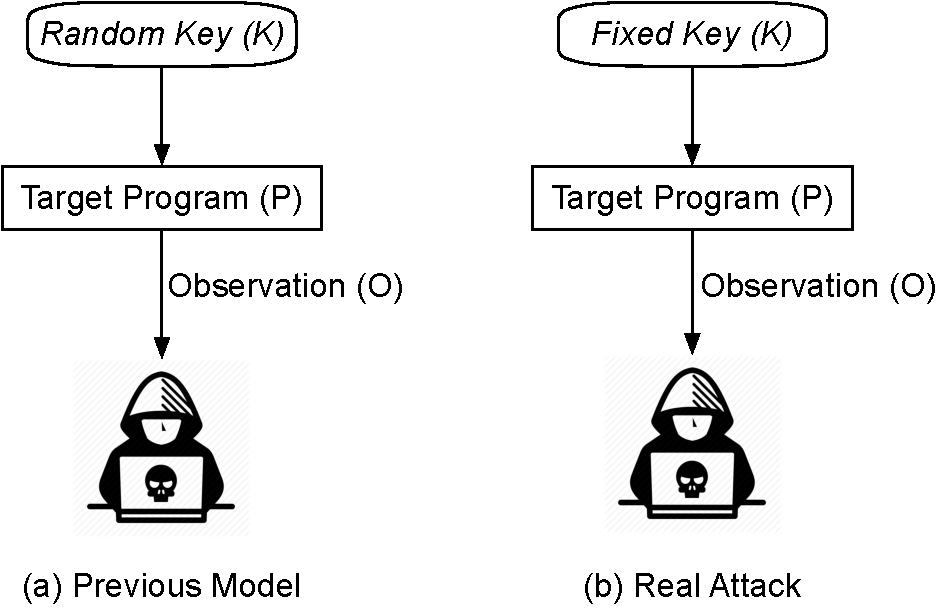
\includegraphics[width=.65\columnwidth]{./figures/chapter4/RA.pdf}
    \caption{The gap between real attacks and previous models}\label{fig:gap}
\end{figure}

\subsection{Precise Analysis}
Now we present our metric to quantify the amount of leaked information from
dynamic analysis.

We assume a program ($\beta$) has $K$ as its sensitive input. The input $K$ should be
a finite set of keys. The program also takes known messages $M$ as its input.
During an AES encryption, for example,
$\beta$ is the encryption function. Here $K$ is the set of all possible AES keys,
and $M$ represents the set consisting of all plaintext messages to be encrypted. In a real execution, an adversary may have
some observations ($O$) of the program. This dissertation only
uses secret-dependent control flows and secret-dependent data
accesses as observations.

With the above definition, we have the following mapping between $\beta$,
$K$, $M$, and $O$:

\begin{displaymath}
    \beta(K, M) \rightarrow O.
\end{displaymath}


We model a side-channel in the following way. An adversary does not have
access to $K$, but he knows $\beta$, $M$, and $O$. For one execution of a
deterministic program, once $k \in K$ and $m \in M$ are fixed, the observation
($o \in O$) should also be determined. An attacker knows $\beta$, $o$,
and $m$. The attacker wants to infer the value of $k$. We use $K^o$ to denote
the set of possible $k$ values that produce the same observation: $K^o = \{ k \in K \, |\, \beta(k, m) \rightarrow o\}$

Then the problem of quantifying the amount of leaked information can be
restated as the following question:

\
\emph{How much uncertainty of $K$ is reduced if an attacker knows $\beta$, $m$, and $o$?}
\

In information theory, the mutual information ($I$) is a measure of the mutual
dependence between two variables. Here we use $I$ to describe the
dependence between original sensitive keys ($K$) and attackers' observations ($O$),
which is defined as

\begin{equation} \label{eq:1}
    I(K;O) = \sum_{k {\in} K}{\sum_{o {\in} O}{p(k, o)\log_2\frac{p(k, o)}{p(k)p(o)}}},
\end{equation}

\noindent where $p(k_i, o_i)$ is the joint discrete distribution of $K$ and $O$.
Alternatively, the mutual information can also be equivalently expressed as

\begin{equation} \label{eq:2}
    I(K;O) = H(K) - H(K|O),
\end{equation}

\noindent where $H(K|O)$ is the entropy of $K$ with the condition $O$. It quantifies the
uncertainty of $K$ given the value of $O$. In other word, the conditional
entropy $H(K|O)$ marks the uncertainty about $K$ after an adversary has gained
some observations ($O$).
\begin{equation}
    H(K|O) = - \sum_{o {\in} O} {p(o) \sum_{k {\in} K}{p(k|o)\log_2p(k|o)}}
\end{equation}

In this research, we hope to give a very precise definition of information
leakages. Suppose an attacker runs the target program with one
fixed input, we want to know how much information he can infer by observing the
memory access patterns ($o$). We come to the simple slogan
~\cite{10.1007/978-3-642-00596-1_21} %% where the information
%% leakage equals:
%% \textbf{Initial uncertainty - remaining uncertainty}
that
\begin{align*}
     & \mathit{Information\ leakage} =                                       \\
     & ~~~~ \mathit{Initial\ uncertainty} - \mathit{Remaining\ uncertainty}.
\end{align*}

Next we compare the Eq.~(\ref{eq:2}) with the above slogan, we find that $H(K)$
is the $\mathit{Initial\ uncertainty}$ and $H(K|O)$ is the $\mathit{Remaining\
        uncertainty}$. During a real attack, the observation ($o$) is known.  Thus we
have $H(K|O) = H(K|o)$.

Therefore, we define the amount of leaked information as
\begin{displaymath}
    Leakage = I(K;o) = H(K) - H(K|o).
\end{displaymath}

For a program ($\beta$) without knowing any domain information, all possible sensitive
inputs should appear equally. Therefore, for any $k \in K$, $p(k) =
    \frac{1}{|K|}$. So we have
$$H(K) = \sum_{k {\in} K}\frac{1}{|K|}\log_2{|K|} = \log_2{|K|}.$$
For any $k' \in K \setminus K^o$, $p(k'|o) = 0$. We get
\begin{align*}
    I(K;o) & = - \sum_{k {\in} K^o}{p(k|o)\log_2p(k|o)}                         \\
           & \qquad   - \sum_{k` {\in} (K \setminus K^o)}{p(k'|o)\log_2p(k'|o)} \\
           & = \sum_{k {\in} K^o}\frac{1}{|K^o|}\log_2{|K^o|}                   \\
           & = \log_2{|K^o|}.
\end{align*}


\begin{mydef}
    \label{chapter4:def}
    Given a program $\beta$ with the input set $K$,
    an adversary has the observation $o$ when the input $k{\in}K^o$.
    We denote it as
    $$\beta(K^o, m) \rightarrow	o.$$

    The amount of leaked information $L_{\beta(k)\rightarrow o}$ based on the observation ($o$) is
    $$L_{\beta(k)\rightarrow o} = \log_2{|K|} - \log_2{|K^o|}.$$
\end{mydef}

The above definition~\cite{AskarovC12} can be understood in an intuitive way. Suppose an attacker
wants to guess a 128-bit encryption key from a program.
Without any domain knowledge,
he can find the key by performing exhaustive search over $2^{128}$ possible keys.
However, the program has a side-channel leakage site. After the program finishes execution, the
attacker gets some leaked information and only needs to find the key by performing
exhaustive search over $2^{120}$ possible keys. Then we can say that 8 bits of the information
is leaked. In this example, $2^{128}$ is the size of $K$ and $2^{120}$ is the size of $K^o$.


With the definition, if an attacker observes that the code in
Figure~\ref{fig:password-checker} runs the branch 1, then the $K^{o^{1}} =
    \{\mathrm{``password"}\}$. Therefore, the information leakage $L_{P(k)=o^{1}} =
    \log_2{2^{64}} - \log_2{1} = 64$ bits, which means the key is totally leaked. If
the attacker observes the code hits branch 2, the leaked information is
$L_{P(k)=o^{2}} = \log_2{2^{64}} - \log_2{(2^{64}-1)} \approx 0$ bit.


We can also calculate the leaked information from the sample code in
Figure~\ref{fig:side-channel}. As the size of input sensitive information is
usually public. The problem of quantifying the leaked information has been
transferred into the problem of estimating the size of input key $|K^o|$ under
the condition $o \in O$. The result is shown in Table~\ref{shtable2}. We can see
that some branches (e.g., A) or traces leak much more information than some others.
These kinds of branches can be vulnerable when an attacker's data is incorporated.
For example, the code will skip some of the calculation if the value is 0 in big
number multiplication.

In contrast, an \emph{average} estimate based on random secret input information is around $1$ bit, as shown in the previous section and Table~\ref{shtable}, is not very useful in practice as an attacker is able to get much more leaked
information in some attack scenarios. As the size of input-sensitive information is
usually public, the problem of quantifying the leaked information is equivalent to the problem of estimating the size of input key $|K^o|$ under
the condition $o \in O$. 

\begin{table}[ht]
    \centering%\small\footnotesize
    \caption{New leakage modeling results}
    \label{shtable2}
    %    \resizebox{\columnwidth}{!}{
    \begin{tabular}{l|cc|cc}
        \hline

        Observation ($o$)         & $A$   & $\neg A$ & $B$   & $\neg B$ \\ \hline
        Number of Solutions       & 65526 & 10       & 32768 & 32768    \\ \hline
        Leaked Information (bits) & 0.0   & 14.7     & 1.0   & 1.0      \\
        \hline
    \end{tabular}
\end{table}

\section{Approximate Model Counting}
\label{MCreasons}
In the previous section, we propose an information leakage definition for realistic attack scenarios to model two types of address-based side-channel leakages and show how to quantify them by calculating the number of input keys ($K^o$) that satisfy the formulas. Intuitively, we can use symbolic execution to capture math formulas and model counting to obtain the number of satisfying input keys ($K^o$). However, some preliminary experiments showed that this approach was far too expensive to use with real-world applications. In this section, we discuss the bottlenecks in this approach and propose a practical solution.


According to Definition~\ref{chapter4:def} introduced in the previous section,
the problem of quantifying the amount of leaked information can be reduced to
the problem of computing the number of items in $K^o$. However, we find that while
there are various propositional model counters (e.g., \#SAT), they are not
sufficiently scalable for production cryptosystem analysis.
Besides, there is no open source modulo theories counter (\#SMT) available.

One straightforward method to approximate the number of solutions is based on Monte Carlo
sampling. However, the number of satisfying values could be exponentially small.
Consider the formula $f_i\equiv{k_1} = 1\land{k_2} = 2\land{k_3} = 3\land{k_4} =
    4$, where $k_1$, $k_2$, $k_3$, and $k_4$ each represents one byte in the
original sensitive input buffer, there is only one satisfying solution of total
$2^{32}$ possible values, which requires exponentially many samples to get a
tight bound. Monte Carlo method also suffers from the curse of dimensionality.
For example, the length of an RSA private key can be as long as 4096 bits. If we
take each byte (8 bits) in the original buffer as one symbol, the formula can
have as many as 512 symbols.

We adopt multiple-step Monte Carlo sampling methods to count the number of
possible inputs that satisfy the logic formula groups. The key idea is to split
these constraints into several small formulas and sample them independently.
We will introduce the method in the following subsection. In this section, we present the algorithm to calculate the information leakage based on Definition~\ref{chapter4:def}. 


\newcommand{\addr}[1]{{l}_{#1}}
\renewcommand{\addr}[1]{{\gamma}_{#1}}
\renewcommand{\addr}[1]{{\zeta}_{#1}}
\renewcommand{\addr}[1]{{\xi}_{#1}}



\subsection{Problem Statement}
For each leakage site, we model it with a constraint using the
method presented in the previous section. Suppose the address of the leakage site is $\addr{i}$, we use $c_{\addr{i}}$ to denote the constraint that models its side-channel leakage. For multiple leakage sites, we take the conjunction of these constraints to represent these leakage sites.

According to Definition~\ref{chapter4:def}, to calculate the amount of leaked
information, the key is to calculate the cardinality
of $K^o$. Suppose an attacker can observe $n$ leakage sites, and each leakage
site has the following constraints: $c_{\addr{1}}, c_{\addr{2}}, \ldots,
    c_{\addr{n}}$ respectively. The total leakage can be calculated from the constraint
$c_t({\addr{1}},{\addr{2}},\ldots,{\addr{n}}) = c_{\addr{1}} \land c_{\addr{2}}
    \land \ldots \land c_{\addr{n}}$.
The problem of estimating the total leaked
information can be reduced to the problem of counting the number of different
solutions that satisfies the constraint
$c_t({\addr{1}},{\addr{2}},\ldots,{\addr{n}})$.
A simple method is to pick elements $k$ from $K$ and check if an
element is also contained in $K^o$. Assume $q$ elements satisfy this condition. In
expectation, we can use $\frac{k}{q}$ to approximate the value of
$\frac{|K|}{|K^o|}$.

However, the above sampling method fails in practice due to the following two problems.

\begin{enumerate}
    \item The curse of dimensionality problem. $c_t({\addr{1}},\ldots,{\addr{n}})$ is
          the conjunction of many constraints. Therefore, the input variables
          of each constraints will also be the input variables of the
          $c_t({\addr{1}},\ldots,{\addr{n}})$. The sampling method fails
          as $n$ grows.
          For example, if the program has $2$ input whose size is
          one byte, the whole search space is a $256^2$ cube. If we want
          the sampling distance between each point equals to $d$, we need
          $256^2d$ points. If the program has $10$ byte input, we need
          $256^{10}d$ points if we still we want the sampling distance equals
          to $d$.

    \item The number of satisfying assignments could be exponentially small.
          According to the Chernoff bound~\cite{hoeffding1994probability}, we need exponentially many samples to
          get a tight bound.
          On an extreme situation, if the constraint only
          has one unique satisfying solution, the simple Monte Carlo method
          cannot find the satisfying assignment even after sampling many
          points.
\end{enumerate}

However, despite the above two problems, we also observe two characteristics of the
problem:
\begin{enumerate}
    \item $c_t({\addr{1}},{\addr{2}},\ldots,{\addr{n}})$ is the conjunction of
          several short constraints $c_{\addr{i}}$. The set containing the
          input variables of $c_{\addr{i}}$ is the subset of the input
          variables of $c_t({\addr{1}},{\addr{2}},\ldots,{\addr{n}})$. Some
          constraints have completely different input variables from other
          constraints.

    \item Each time when we sample $c_t({\addr{1}},{\addr{2}},\ldots,{\addr{n}})$
          with a point, the sampling result is \emph{Satisfied} or not \emph{Not Satisfied}.
          The outcome does not depend on the result of
          previous experiments. Also, as the amount of leaked information is calculated
          by a $\log$ function, we need not exactly count the number of solutions for
          a given constraint.


\end{enumerate}

In regard to the above problems, we present our methods. First, we split
$c_t(\addr{1},\addr{2},\ldots,\addr{n})$ into several independent constraint
groups. After that, we run a multi-step sampling method for each constraint.

\subsection{Maximum Independent Partition}

For a constraint $c_{\addr{i}}$, we define function $\pi$, which projects the
constraint into a set of different input symbols. For example, $\pi(k1 + k2 >
    128) = \{k1, k2\}$.

\begin{mydef}[]
    \label{independentC}
    Given two constraints $c_m$ and $c_n$, we call them independent iff
    $$\pi(c_m) \cap \pi(c_n) = \emptyset.$$
\end{mydef}

Based on Definition~\ref{independentC}, we can split the constraint
$c_t(\addr{1},\addr{2},\addr{3},\ldots,\addr{n})$ into several independent constraints.
There are many partitions. For our project, we are interested in the following
one.

\begin{mydef}\label{Goodpartition}
    For the constraint $c_t(\addr{1},\addr{2},\ldots,\addr{n})$,
    we call the constraint group
    $g_{1}, g_{2}, \ldots, g_{m}$
    the maximum independent partition of $c_t(\addr{1},\addr{2},\ldots,\addr{n})$ iff
    \begin{enumerate}
        \item $g_{1} \land g_{2} \land \ldots \land g_{m} = c_t(\addr{1},\addr{2},\ldots,\addr{n})$,
        \item $\forall i, j \in \{1, \ldots, m\} \quad \textrm{and} \quad
                  i \neq j,\quad\pi(g_{i}) \cap \pi(g_{j}) = \emptyset $,
        \item For any other partitions  $h_{1}, h_{2}, \ldots, h_{m'}$ satisfy 1) and
              2), $m \geq m'$.
    \end{enumerate}

\end{mydef}

The reason we want a good partition of constraints is we want to reduce
the dimensions. For example,
a good partition of $F: ({k_1} = 1)\land({k_2} = 2)\land({k_3} > 4)\land({k_3} - {k_4} > 10)$ would be
$g_{1}: ({k_1} = 1)\quad g_{2}: ({k_2} = 2)\quad g_{3}: ({k_3} > 4) \land
    ({k_3} - {k_4} > 10)$
We can sample each constraint independently and combine them
with Theorem~\ref{IndependentConstraint}.

\begin{theorem}
    \label{IndependentConstraint}
    Let $g_{1}, g_{2}, \ldots, g_{m}$ be a maximum independent partition of
    $c_t(\addr{1},\addr{2},\ldots,\addr{n})$.
    $K_c$ is the input set that satisfies constraint $c$. We have the following
    equation with regard to the size of $K_c$
    $$|K_{c_t(\addr{1},\addr{2},\ldots,\addr{n})}| = |K_{g_{1}}| \cdot |K_{g_{2}}| \cdot \ldots \cdot|K_{g_{n}}|.$$
\end{theorem}
With Theorem~\ref{IndependentConstraint}, we transfer the problem of counting the number of solutions to a complicated constraint in a high-dimension
space into counting solutions to several small constraints. We compute the maximum independent partition by iterating each $\addr{i}$ and applying the function $\pi$ over the constraint $\addr{i}$.

We apply 
Algorithm~\ref{algo:max-inde} to get the Maximum Independent Partition of the
$c_t(\addr{1},\addr{2},\ldots,\addr{n})$.


\IncMargin{1em}
\begin{algorithm}[th]\normalsize
    \DontPrintSemicolon
    \SetKwInOut{Input}{input}\SetKwInOut{Output}{output}
    \Input{$c_t(\addr{1},\addr{2},\ldots,\addr{n}) = c_{\addr{1}} \land c_{\addr{2}} \land \ldots \land c_{\addr{m}}$}
    \Output{The Maximum Independent Partition of $G = \{g_{1}, g_{2}  , \ldots,  g_{m} \}$ }
    Insert $c_{\addr{1}}$ to $G$ as a new entry \;
    \For{$i\leftarrow 2$ \KwTo $n$}
    {
        $S_{c_{\addr{i}}}$ $\leftarrow$ $\pi(c_{\addr{i}})$ \;
        \For{$g_{i} \in G$}
        {
            $S_{g_j}$ $\leftarrow$ $\pi(g_{j})$ \;
            $S$ $\leftarrow$ $S_{c_{\addr{i}}} \cap S_{g_j}$  \;
            \If{$S \neq \emptyset$}
            {
                $g_{j} \leftarrow g_{i} \land g_{\addr{i}}$ \;
                \textbf{continue} \;
            }
            Insert $c_{\addr{i}}$ to $G$ as a new entry \;
        }
    }
    \caption{The Maximum Independent Partition}
    \label{algo:max-inde}
\end{algorithm}
\DecMargin{1em}


\subsection{Multiple-step Monte Carlo Sampling}

After we split these constraints into several small constraints, we count the number of solutions for each constraint. Even though the dimension has been
significantly reduced by the previous step, this is still a \#P problem. For our project, we apply the approximate counting instead of exact counting for two reasons. First, we do not need to have a very precise result of the exact number of total solutions since the information is defined with a logarithmic function. We do not need to distinguish between constraints having $10^{10}$ or $10^{10} + 10$ solutions; they are very close to after taking logarithmic. Second, the
precise model counting approaches, such as Davis-Putnam-Logemann-Loveland (DPLL)
search, have difficulty scaling up to large problem sizes.

We apply the ``counting by sampling'' method. For
the constraint $g_{i}= c_{i_1} \land c_{i_2} \land ,\ldots, \land c_{i_j}\\ \land ,\ldots, \land c_{i_m}$, if the solution satisfies $g_{i}$, it should also
satisfy any constraint from $c_{i_1}$ to $c_{i_m}$. In other words, $K_{c_gi}$
should be the subset of $K_{c_1}$, $K_{c_2}$, \ldots , $K_{c_m}$. We notice that
$c_i$ usually has fewer inputs than $g_{i}$. For example, if
$c_{i_j}$ has only one 8-bit input variable, we can find the exact solution set
$K_{c_{i_j}}$ of $c_{i_j}$ by trying every possible 256 solution. After that,
we only generate random input numbers for the other input variables in
constraint $g_{i}$. With this simple yet effective trick, we reduce the number of inputs while still ensuring accuracy. The details of the algorithm is shown in Algorithm~\ref{chapter4:alg2}.


\IncMargin{1em}
\begin{algorithm}\normalsize
    \SetAlgoLined
    \DontPrintSemicolon

    \KwIn{{The constraint $g_{i}= c_{i_1} \land c_{i_2}
                    \land \ldots \land c_{i_m}$}}
    \KwOut{{The number of assignments that satisfy $g_{i}$ $|K_{g_{i}}|$}}

    $n$: the number of sampling times \;
    $S_{c_i}$: the set contains input variables for $c_{i}$ \;
    $n_{s}$: the number of satisfying assignments \;
    $N_{c_t}$: the set contains all solution for $c_t$ \;
    $r$: times of reducing $g$\;
    $k$: the input variable \;
    $R$: a function that produces a random point from $S_{c_i}$\;
    %$\#k$: the satisfying number of k \fixme{this number is not used syntactically} \;
    %Initialization: \;
    $r$ $\leftarrow$ $1$,
    $n$ $\leftarrow$ $0$ \;
    \For{$t$ $\leftarrow$ $1$ \KwTo $m$} {
    $S_{c_t}$ $\leftarrow$ $\pi(c_t)$ \;
    \If{$|S_{c_t}| = 1$}
    {
    $N_{c_t}$ $\leftarrow$ Compute all solutions of $c_i$ \;
    $N_{c_t} = \{n_1, \ldots, n_m\},\ S_{c_t} = \{k\}  $ \;
    $g_{i} = $ $g_i(k=n_1) \land \ldots \land g_i(k=n_m)$ \;
    $r \leftarrow r+1$ \;

    }
    }
    \While{$n \leq \frac{8p}{1-p}$} {
        $S_{g_i}$ $\leftarrow$ $\pi(g_i)$ \;
        $v \leftarrow R(S_{g_i})$ \;
        \If{$v$ satisfies $g_i$}
        {
            $n_s \leftarrow n_s + 1$
        }
        $n \leftarrow n +1,\ p = \frac{n_s}{n}$
    }

    $|K_{g_{i}}|$ $\leftarrow$ $n_s|K| / (n * r * \mathrm{range(k)})$
    \caption{Multiple Step Monte Carlo Sampling}\label{chapter4:alg2}
\end{algorithm}
\DecMargin{1em}

\subsection{Error Estimation}
\label{sssec:errest}
Our result has a probabilistic guarantee that the error of the estimated amount of leaked
information is less than 1 bit under the Central Limit Theorem (CLT) and uncertainty
propagation theorem~\cite{walpole1993probability}.

Let $n$ be the number of samples and $n_s$ be the number of samples that satisfy
the constraint $C$. Then we get $\hat{p} = \frac{n_s}{n}$. If we repeat the
experiment multiple times, each time we get a $\hat{p}$. As each
$\hat{p}$ is independent and identically distributed, according to the central limit
theorem, the mean value should follow the normal distribution
$$ \frac{\bar{p}-E(p)}{\sigma\sqrt{n}} \rightarrow N(0,1). $$ Here $E(p)$ is the
mean value of $p$, and $\sigma$ is the standard variance of $p$. If we use the
observed value $\hat{p}$ to calculate the standard deviation, we can claim that
we have 95\%\footnote{For a normal distribution, 95\% of variable $\Delta p$ fall within two sigmas of the mean.}
confidence that the error $\Delta p= \bar{p} - E(p)$ falls in the interval:
$$ |\Delta p| \leq 1.96\sqrt{\frac{ \hat{p} (1- \hat{p} )}{n}}.$$

Since we use $L = \log_{2}p$ to estimate the amount of leaked information, we
can have the following error propagation formula $\Delta L = \frac{\Delta
        p}{p\ln2}$ by taking the derivative from Definition~\ref{chapter4:def}. For \tool, we want the error of estimated leaked
information ($\Delta L$) to be less than 1 bit. So we get $\frac{\Delta
        p}{p\ln2} \leq 1$. Therefore, as long as $$ n \geq \frac{1.96^2(1-p)}{p(\ln2)^2},$$ 
\noindent we have 95\% confidence that the error of estimated leaked information is less than 1 bit.
During the simulation, if $n$ and $p$ satisfy this inequality, the Monte Carlo
simulation will terminate.

\section{Design and Implementation}

Figure~\ref{fig:workflow} shows the three steps of \tool{}.
First, we run the target program with a
concrete input (sensitive information) under the dynamic binary instrumentation
(DBI) framework to collect an execution trace. After that, we run the symbolic
execution to capture fine-grained semantic information for each
secret-dependent control-flow transfer and data access. Finally, we run Monte
Carlo (MC) simulation to estimate the amount of leaked information.

\begin{figure}[ht]
    \centering
    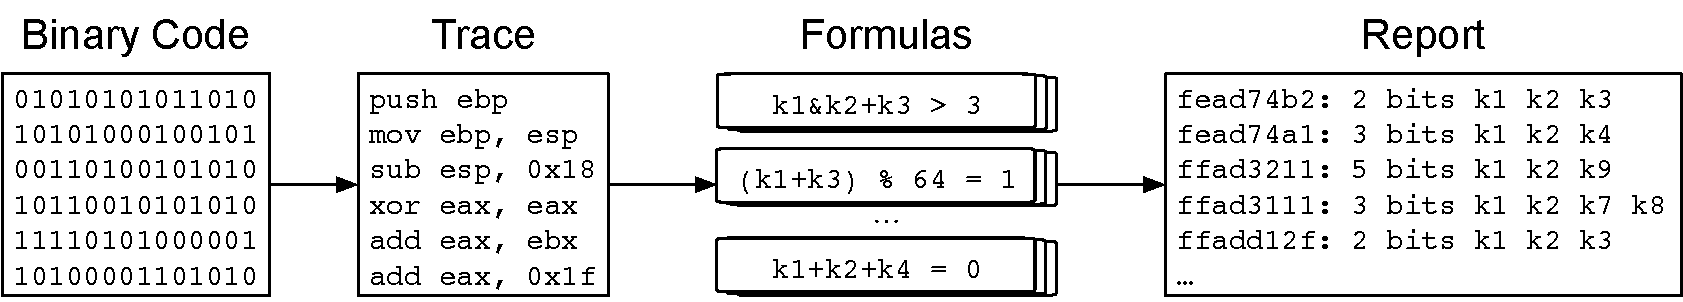
\includegraphics[width=0.95\textwidth]{./figures/chapter4/workflow.pdf}
    \caption{The workflow of \tool{}.}
    \label{fig:workflow}
\end{figure}

\subsection{Execution Trace Generation} The design goal of \tool{} is to estimate the information leakage as precisely as possible.
We run the target binary under a dynamic binary instrumentation (DBI) tool
to record execution traces and runtime information.
Once the sensitive information is loaded into memory, we start to collect the trace.
In this step, we mark variables and buffers that hold the sensitive data by either annotating the source code (\textsf{make\_abacus\_symbolic}) or telling the DBI tool of the memory address and the length of secrets.

\subsection{Instruction Level Symbolic Execution} We model an attacker's
observations from side-channel vulnerabilities with logic formulas.
Each formula captures the fine-grained information between the input
secrets and leakage sites. The engine only symbolically executes
instructions that might be affected by the input sensitive data. \tool{} works on one path at a time. The memory model is conceptually similar to other offline executors (e.g., SAGE~\cite{godefroid2008automated} and the trace-based executor of BitBlaze~\cite{song2008bitblaze}). That is, we use symbolic execution to track secrets. When secrets are loaded into the memory, \tool{} starts to interpret instructions symbolically. We treat secrets as symbols ($S$). For other variables, we use concrete values ($C$) from the execution. We do not know which instruction may manipulate a secret until we execute it. For each instruction, if all its operands and implicit memory accesses are concrete values, we perform concrete calculation and update the destination with the concrete value according to the instruction semantics. Otherwise, we symbolically interpret the instruction and update the destination with a formula.

\subsection{Leakage Estimation} 
We change the information leakage quantification problem into a counting problem. We propose a
Monte Carlo method to estimate the number of satisfying solutions. With the help of the Central Limit Theorem (CLT), we also give an error
estimate with the probability, which provides us with the \emph{precision guarantee}.

\subsection{Implementation}

\tool{} consists of 16,729 lines of code in C++17 and Python. It has three components: an Intel Pin tool that collects the execution trace, the
instruction-level symbolic execution engine, and the back-end that estimates the information leakage. Table~\ref{tbl:implementation} shows the breakdown of the implementation of \tool{}.

\begin{table}[ht]
    \centering\normalsize
    %    \resizebox{.8\columnwidth}{!}{
    \caption{\tool{}' main components and sizes}\label{tbl:implementation}
    \begin{tabular}{lr@{~}l}
        \hline
        Component            & \multicolumn{2}{c}{Lines of Code (LOC)}             \\ \hline
        Trace Logging        & 501 lines                               & of C++    \\
        Symbolic Execution   & 14,963 lines                            & of C++    \\
        Data Flow            & 451 lines                               & of C++    \\
        Monte Carlo Sampling & 603 lines                               & of C++    \\
        Others               & 211 lines                               & of Python \\ \hline
        Total                & 16,729 lines                            &           \\\hline
    \end{tabular}
    %    }
\end{table}

Our current implementation supports most Intel 32-bit instructions that are essential to find address-based side-channel vulnerabilities, including bitwise operations, control transfer, data movement, and logic instructions. The tool uses concrete values to update the registers and memory for instructions that the implementation does not support. Therefore, the tool may miss some leakages but will not raise false positives.

\section{Evaluation}
\begin{table}[]
    \centering
    \small
    \caption{Evaluation results overview: Side-channel Leaks\,(Leaks),
        Secret-dependent Control-flows\,(CF), Secret-dependent Data-flows\,(DF),
        the number of instructions\,(\# Instructions), Symbolic Execution\,(SE) and Monte Carlo\,(MC) time.
    }\label{chapter4:table:over_result}

    %    \resizebox{1.9\columnwidth}{!}{
    \begin{threeparttable}
    \renewcommand\TPTminimum{\linewidth}
   % \captionsetup{font=small}
    \makebox[\linewidth]{
        \begin{tabular}{lrrrrrr}
            \hline
            \textbf{Name}     & \textbf{\# Leaks}        & \textbf{\# CF} & \textbf{\# DF}
                              & \textbf{\# Instructions} & \textbf{Detection}    & \textbf{Quantification}                                      \\\hline
                              &                          &                &                &             & ms      & ms      \\\cline{6-7}
            AES\tnote{1}      & 68                       & 0              & 68             & 39,855      & 512     & 1,052   \\
            AES\tnote{2}      & 68                       & 0              & 68             & 39,855      & 520     & 1,057   \\
            AES\tnote{4}      & 75                       & 0              & 75             & 1,704       & 231     & 9,199   \\
            AES\tnote{5}      & 88                       & 0              & 88             & 1,350       & 36      & 1,924   \\
            AES\tnote{6}      & 88                       & 0              & 88             & 1,350       & 35      & 1,961   \\
            AES\tnote{7}      & 88                       & 0              & 88             & 1,420       & 36      & 2,161   \\
            AES\tnote{8}      & 88                       & 0              & 88             & 1,586       & 43      & 1,631   \\
            DES\tnote{1}      & 15                       & 0              & 15             & 4,596       & 58      & 162     \\
            DES\tnote{2}      & 15                       & 0              & 15             & 4,596       & 57      & 162     \\
            DES\tnote{4}      & 6                        & 0              & 6              & 2,976       & 163     & 4,677   \\
            DES\tnote{5}      & 8                        & 0              & 8              & 2,593       & 166     & 6,509   \\
            DES\tnote{6}      & 8                        & 0              & 8              & 2,593       & 165     & 5,975   \\
            DES\tnote{7}      & 8                        & 0              & 8              & 4,260       & 182     & 5,292   \\
            DES\tnote{8}      & 6                        & 0              & 6              & 8,272       & 229     & 5,152   \\
                              &                          &                &                &             & seconds & seconds \\\cline{6-7}
            Chacha20\tnote{3} & 0                        & 0              & 0              & 149,353     & 2       & 0       \\
            Poly1305\tnote{3} & 0                        & 0              & 0              & 1,213,937   & 15      & 0       \\
            Argon2i\tnote{3}  & 0                        & 0              & 0              & 4,595,142   & 37      & 0       \\
            Ed25519\tnote{3}  & 0                        & 0              & 0              & 5,713,619   & 271     & 0       \\
            ECDSA\tnote{1}    & 6                        & 6              & 0              & 4,214,946   & 48      & 31      \\
            ECDSA\tnote{2}    & 4                        & 4              & 0              & 4,192,558   & 102     & 1639    \\
            ECDSA\tnote{5}    & 5                        & 4              & 1              & 8,248,322   & 101     & 62      \\
            ECDSA\tnote{6}    & 5                        & 4              & 1              & 8,263,599   & 100     & 58      \\
            ECDSA\tnote{7}    & 5                        & 4              & 1              & 6,100,465   & 76      & 42      \\
            ECDSA\tnote{8}    & 0                        & 0              & 0              & 10,244,076  & 121     & 0       \\
            ECDSA\tnote{9}    & 0                        & 0              & 0              & 9,266,191   & 102     & 59      \\


                              &                          &                &                &             & minutes & minutes \\\cline{6-7}
            RSA\tnote{1}      & 6                        & 6              & 0              & 22,109,246  & 39      & 41      \\
            RSA\tnote{2}      & 12                       & 12             & 0              & 24,484,441  & 44      & 251     \\
            RSA\tnote{4}      & 107                      & 105            & 2              & 17,002,523  & 23      & 428     \\
            RSA\tnote{5}      & 38                       & 27             & 11             & 14,468,307  & 29      & 436     \\
            RSA\tnote{6}      & 36                       & 27             & 9              & 15,285,210  & 40      & 714     \\
            RSA\tnote{7}      & 31                       & 22             & 9              & 16,390,750  & 34      & 490     \\
            RSA\tnote{8}      & 4                        & 4              & 0              & 18,207,016  & 8       & 53      \\
            RSA\tnote{9}      & 8                        & 8              & 0              & 18,536,796  & 5       & 780     \\
            RSA\tnote{10}     & 11                       & 9              & 2              & 9,527,231   & 2       & 38      \\
            RSA\tnote{11}     & 14                       & 14             & 0              & 10,513,606  & 14      & 503     \\
            RSA\tnote{12}     & 8                        & 8              & 0              & 27,407,986  & 113     & 6560    \\

            Total             & 904                      & 241            & 663            & 167,141,947 & 341m    & 10,232m \\\hline
        \end{tabular}}
    \end{threeparttable}
    \begin{tablenotes}
        \scriptsize

        \item[1] mbedTLS\,2.5  \,~~~~~\item[2] mbedTLS\,2.15 ~\item[3] Monocypher\,3.0 \\
        \item[4] OpenSSL\,0.9.7  ~~~\item[5] OpenSSL\,1.0.2f  \item[6] OpenSSL\,1.0.2k 
        \item[7] OpenSSL\,1.1.0f ~\item[8] OpenSSL\,1.1.1 ~\item[9] OpenSSL\,1.1.1g \\
        \item[10] Libgcrypt\,1.6.1 ~\item[11] Libgcrypt\,1.7.3 \item[12] Libgcrypt\,1.8.5\\
    \end{tablenotes}

\end{table}

\subsection{Overview}
In this section, we evaluate \tool{} on a set of popular crypto libraries.
In particular, we are interested in following aspects:
\begin{itemize}
\item Can \tool{} precisely report the number of leaked bits in crypto
          libraries? 
\item Are the numbers of leaked bits reported by \tool{} useful
          to justify the severity levels of the side-channel vulnerabilities?
\end{itemize}

Our testbed is comprised of several popular cryptography libraries. We choose them based
on the following aspects. First, they should be widely used in many popular software.
In general, it is hard to implement a secure cryptography library from scratch. So most
software only use a few number of different cryptography libraries. Second, we choose some
libraries which are well studied in the previous work. We can refer to these conclusions to
verify our results. Based on the two requirements, we evaluate \tool{} on the following libraries:
OpenSSL, Libgcrypt, mbedTLS, Monocypher. OpenSSL, Libgcrypt, and mebdTLS are the most widely used
cryptography libraries. OpenSSL and mbedTLS have been widely studied in the previous research.
Monocyper is designed to be side-channel resistant. We use the library to test if our tool has any
false positives. We also test \tool{} on some simple countermeasure implementations. 

We write simple encryption and decryption function with the above libraries. After that, we build
the source code into 32-bit binary executions. The configuration of our experiment is shown as follows.
\begin{itemize}
\item CPU: 2.90GHz Intel Xeon(R) E5-2690 CPU
\item Memory: 128 GB
\item OS: Ubuntu 18.04 LTS
\item Compiler: GCC 7.5
\end{itemize}

Table~\ref{chapter4:table:over_result} shows an overview of the evaluation results. 
\tool{} also finds that most side-channel
vulnerabilities leak very little information, which confirms our
initial assumption.  
However, \tool{} finds some vulnerabilities with severe
leakages. Prior research has confirmed that some of these
vulnerabilities can be exploited in real attacks.
With our tool, developers can
distinguish non-critical ``vulnerabilities'' from the severe ones.

Symmetric encryption implementations in OpenSSL and mbedTLS have significant leakage due to their lookup table implementations. 
\tool{} confirms that these leakage comes from table lookups. The new implementation of OpenSSL has adopted several methods (e.g., one single S-box instead of four lookup tables, smaller lookup tables) to mitigate the problem. These changes are rather easy but significantly decrease the total amount of leaked information as the quantification result indicates.

\tool{} can estimate how
much information is leaked from each vulnerability. During the evaluation,
for each leakage site, \tool{} will stop once 1) it has 95\% confidence
that the error of the estimated leaked information is less than 1 bit,
which gives the leakage quantification a \emph{precision guarantee}, 
or 2) it cannot reach the termination condition after 10 minutes.  In
the latter case, it means \tool{} cannot estimate the amount of leakage with a
probabilistic guarantee. \tool{} times out on around 10\% reported side-channel leakage sites. We manually check these leakage sites and find most of them are quite severe.
We will present the details in the subsequent sections.

\subsection{Case Studies}

\subsubsection{Symmetric Ciphers: DES and AES}\label{eval:sym}
We test both DES and AES ciphers from mbedTLS and OpenSSL\@. Both cipher implementations apply lookup tables, which improve performance but can also introduce side-channels as well. During our evaluation, we find mbedTLS 2.5 and 2.15.1 have the same implementation of AES and DES\@. Therefore, our tool reports the same leakages for both versions.

We find that the DES implementations in both mbedTLS and OpenSSL have several severe information leakages in the key-schedule function. We do not see any mitigation
in the new version. We think it is not seen as worth the engineering efforts given the life cycles of DES\@.

\tool{} shows that the AES in OpenSSL 1.1.1 has less leakage than other versions.
OpenSSL 1.1.1 uses 1KB lookup tables with 8-bit entries, unlike older versions that use a table with 32-bit entries. Our tool suggests a smaller lookup table might mitigate side-channel vulnerabilities.

During our evaluation, we find mbed TLS 2.5 and 2.15.1 have the same
implementation of AES\@. Our tool provides the same leakage report for both
versions. \tool{} identifies that most leakages are in function
\emph{mbedtls\_internal\_aes\_decrypt}. (Other leakage sites are in function
\emph{mbedtls\_aes\_setkey\_enc}.) All leakages are caused by the secret-dependent
memory accesses. Shown in Figure~\ref{mbedtls_aes}, there are seven leakage
sites in total. Leakage 1, 2, 3 are the same and leakage 4, 5, 6, 7 are the
same. They both use a pre-computed lookup table to speed up computation.
However, \tool{} reports leakage 1, 2, 3 typically leak more information (7.6 - 8.1 bits)
compared to leakage 4, 5, 6, 7 (4.0 bits). We check the source code and find leakage 1, 2,
3 use secret to access the lookup table \emph{RT0, RT1, RT2, RT3}, which is 8K
each. On the contrary, leakage 4, 5, 6, 7 each accesses a smaller lookup table
(2K). Therefore, leakage 4, 5, 6, 7 leak less information.

\begin{figure}%[h!]
    \centering
    \begin{lstlisting}[frame=none]
int mbedtls_internal_aes_encrypt(mbedtls_aes_context *ctx,
const unsigned char input[16],
unsigned char output[16] )
{
uint32_t *RK, X0, X1, X2, X3, Y0, Y1, Y2, Y3;
...
for( i = ( ctx->nr >> 1 ) - 1; i > 0; i-- )
{
    AES_FROUND( Y0, Y1, Y2, Y3, X0, X1, X2, X3 );   // Leakage 1
    AES_FROUND( X0, X1, X2, X3, Y0, Y1, Y2, Y3 );   // Leakage 2
}
AES_FROUND( Y0, Y1, Y2, Y3, X0, X1, X2, X3 );       // Leakage 3
X0 = *RK++ ^ \                                      // Leakage 4
    ( (uint32_t) FSb[ ( Y0       ) & 0xFF ]       ) ^
    ( (uint32_t) FSb[ ( Y1 >>  8 ) & 0xFF ] <<  8 ) ^
    ( (uint32_t) FSb[ ( Y2 >> 16 ) & 0xFF ] << 16 ) ^
    ( (uint32_t) FSb[ ( Y3 >> 24 ) & 0xFF ] << 24 );
// X1, X2, X3 do the same computation as X0
...                                                 // Leakage 5,6,7
PUT_UINT32_LE( X0, output,  0 );
...
return 0;
}
\end{lstlisting}
    \caption{Function \textit{mbedtls\_internal\_aes\_encrypt}}
    \label{mbedtls_aes}
\end{figure}

\subsubsection{Asymmetric Ciphers: RSA}\label{eval:asym}

\begin{figure*}
    \centering
    \subfloat[OpenSSL 0.9.7]{
        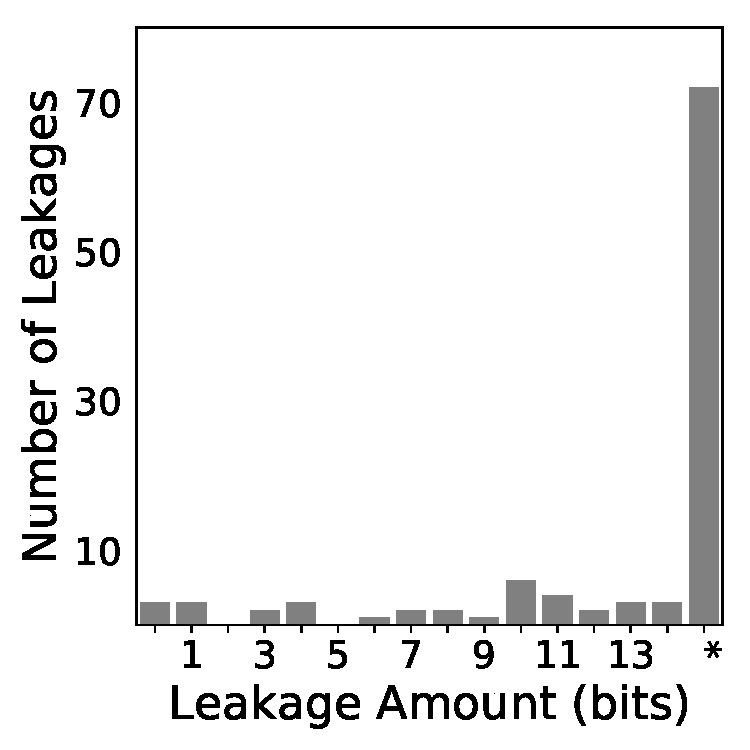
\includegraphics[width=.3\linewidth]{./figures/chapter4/result/RSA-openssl-0-9-7.pdf}
        \label{fig:rsa-1}
    }
    \subfloat[OpenSSL 1.0.2f]{
        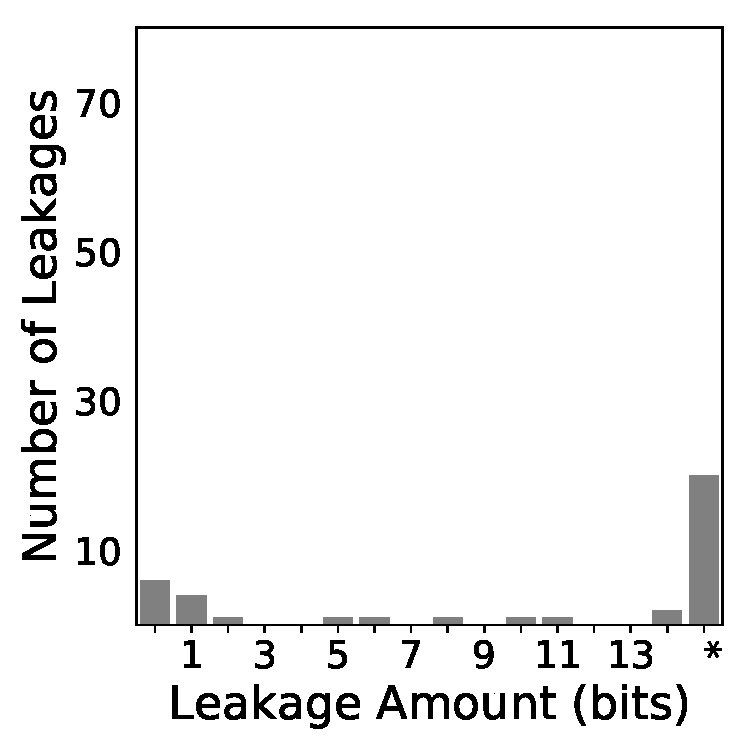
\includegraphics[width=.3\linewidth]{./figures/chapter4/result/RSA-openssl-1-0-2f.pdf}
        \label{fig:rsa-2}
    }
    \subfloat[OpenSSL 1.0.2k]{
        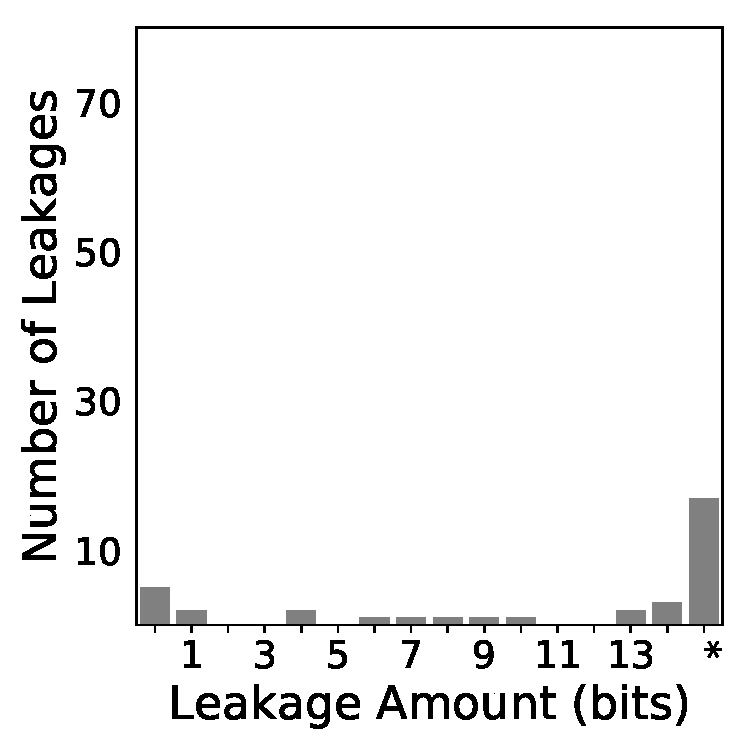
\includegraphics[width=.3\linewidth]{./figures/chapter4/result/RSA-openssl-1-0-2k.pdf}
        \label{fig:rsa-3}
    }
        \hfill

    \subfloat[OpenSSL 1.1.0f]{
        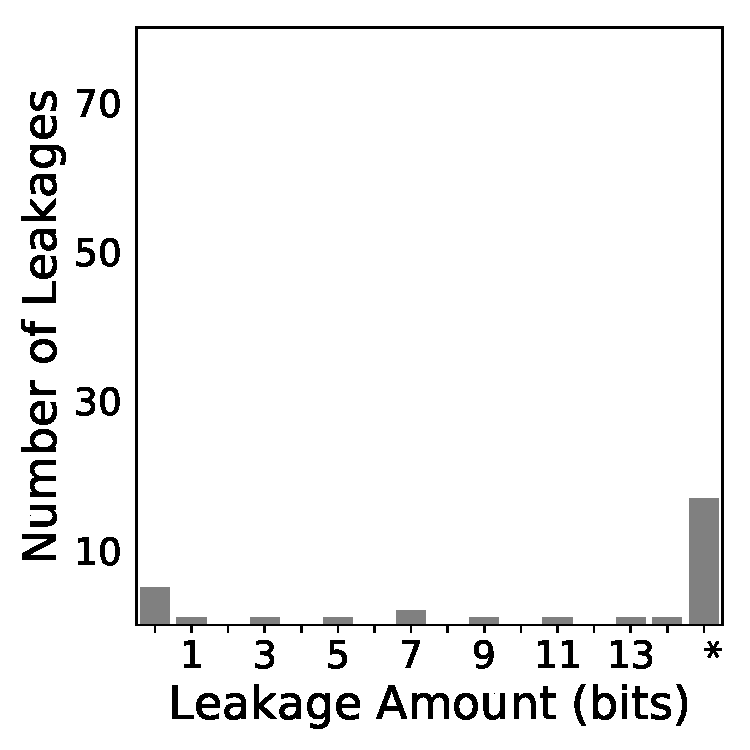
\includegraphics[width=.3\linewidth]{./figures/chapter4/result/RSA-openssl-1-1-0f.pdf}
        \label{fig:rsa-4}
    }
    \subfloat[OpenSSL 1.1.1]{
        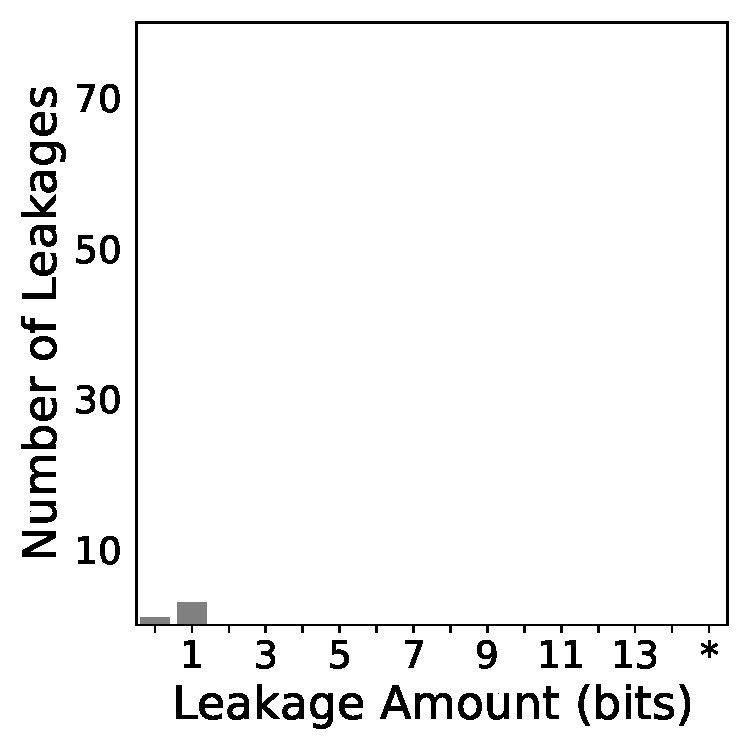
\includegraphics[width=.3\linewidth]{./figures/chapter4/result/RSA-openssl-1-1-1.pdf}
        \label{fig:rsa-5}
    }
    \subfloat[OpenSSL 1.1.1g]{
        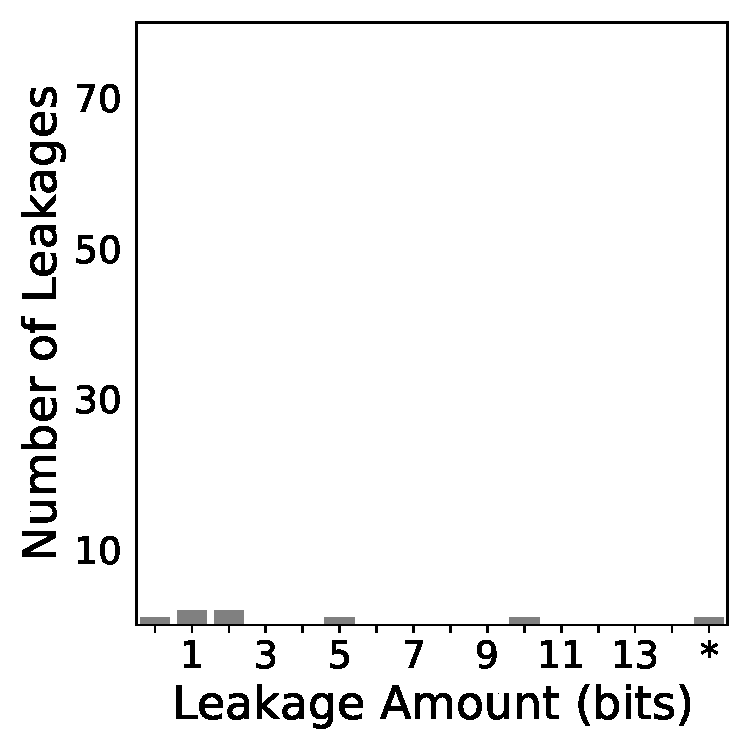
\includegraphics[width=.3\linewidth]{./figures/chapter4/result/RSA-openssl-1-1-1g.pdf}
        \label{fig:rsa-6}
    }
    \caption{Side-channel leakages in different implementations of RSA in OpenSSL\@. 
        We round the number of leaked information into the nearest integer. 
        The mark $*$ means timeout.}
    \label{fig:rsa}
\end{figure*}
We also evaluate \tool{} on RSA.  %, which is available online at the tool release website.
%% \jl{where?}. In general,
%% developers are interested in fixing side-channel vulnerabilities for the RSA implementations.
%% \jl{Then maybe find some space to present these results?}
 As shown in Figure~\ref{fig:rsa}, the result indicates that the newer
versions of OpenSSL leak less information than the earlier
versions. After version 0.9.7g, OpenSSL adopts a fixed-window \textsf{mod\_exp\_mont}
implementation for RSA\@. With this design, the sequence of squares and
multiples and the memory access patterns are independent of the secret key.
\tool{}'s result confirms the new exponentiation implementation has mitigated 
most leakages effectively because the four newer versions have fewer
leakages than version 0.9.7, which introduced this change.
OpenSSL version 1.0.2f, 1.0.2k, and 1.1.0f almost have the
same amount of leakage. We check the ChangeLog and find only one change to
patch vulnerability CVE-2016-0702. 
\tool{} finds OpenSSL 1.1.1 and 1.1.1g have significantly less
leaked information than other versions.
We check the ChangeLog of these two versions and find a claim that
the new RSA implementation adopts ``numerous side-channel attack mitigation'', 
which proves the effectiveness of our quantifying method.
%We also observe the latest version (1.1.1g) contains some new leakages. We have
%contacted the developers and they have confirmed our findings.



Our quantification result shows vulnerabilities
that leak significant amounts of information
are more likely to be fixed in the updated version.
As presented in Figure~\ref{fig:rsa}, 
OpenSSL 0.9.7 has several severe leaks from
function \textsf{bn\_sqr\_comba8}, which is a main 
component of the OpenSSL big number implementation.
Shown in Figure~\ref{fig:old_sqr2}, it has a 
secret-dependent control flow at line 8.
The value of the function parameter \texttt{a} is derived from
the secret key. 
As function \textsf{bn\_sqr\_comba8}
calls the macro (\textsf{sqr\_add\_c2}) multiple times, 
and the code can leak some information each time.
\tool{} indicates the vulnerability is quite severe. 
It was patched in OpenSSL 1.1.1\@. In 
Figure~\ref{fig:new_sqr2}, control-flows transfers are replaced
so there are no leaks in the function
\textsf{sqr\_add\_c2} in OpenSSL 1.1.1\@. We note
that line 4 and 9 in Figure~\ref{fig:old_sqr2} both contain \texttt{if} branches.
However, they are not leaks because
most compilers use \emph{add with carry} instruction to eliminate the branch.
In addition, branches can be compiled into non-branch machine instructions 
with conditional moves. 
We notice a bitwise operation in Libgcrypt 1.8.5 is compiled to a conditional 
jump, which leads to a side-channel leakage.
Therefore, source-level code reviews are not accurate
enough to detect side-channels. 

For vulnerabilities that leak less amount of information,
developers are more reluctant to fix them or fixing them unintentionally. For example, OpenSSL 0.9.7 adds a fixed windows version of function \textsf{BN\_mod\_exp\_mont\_consttime} to replace original function \textsf{BN\_mod\_exp\_mont}.
\tool{} detects a minor vulnerability in the original function that can leak the last bit of the big number \texttt{m}. In the updated version, developers make the fixed windows the default option and rewrite most of the function. However, the leakage site still exists in OpenSSL 1.1.1.
\begin{figure}
    \centering
    \begin{lstlisting}[xleftmargin=.08\textwidth, xrightmargin=.0\textwidth, frame=none]
# define mul_add_c2(a,b,c0,c1,c2)                    \
    t=(BN_ULLONG)a*b;                                \
    tt=(t+t)&BN_MASK;                                \
    if (tt < t) c2++;                                \
    t1=(BN_ULONG)Lw(tt);                             \
    t2=(BN_ULONG)Hw(tt);                             \
    c0=(c0+t1)&BN_MASK2;                             \
    if ((c0 < t1) && (((++t2)&BN_MASK2) == 0)) c2++; \
    c1=(c1+t2)&BN_MASK2; if ((c1) < t2) c2++;
\end{lstlisting}
    \caption{Macro \textsf{sqr\_add\_c2} in OpenSSL 0.9.7}
    \label{fig:old_sqr2}
\end{figure}


\begin{figure}
    \centering
    \begin{lstlisting}[xleftmargin=.08\textwidth, xrightmargin=.0\textwidth, frame=none]
# define mul_add_c2(a,b,c0,c1,c2)      do { \
    BN_ULONG ta = (a), tb = (b);            \
    BN_ULONG lo, hi, tt;                    \
    BN_UMULT_LOHI(lo,hi,ta,tb);             \
    c0 += lo; tt = hi+((c0<lo)?1:0);        \
    c1 += tt; c2 += (c1<tt)?1:0;            \
    c0 += lo; hi += (c0<lo)?1:0;            \
    c1 += hi; c2 += (c1<hi)?1:0;            \
    } while(0)
\end{lstlisting}
\caption{Macro \textsf{sqr\_add\_c2} in OpenSSL 1.1.1}
\label{fig:new_sqr2}
\end{figure}

To evaluate the effectiveness of the leaked bits reported by \tool{}, we conduct a case study of all the leaked sites identified by \tool{} in OpenSSL 1.1.0f. Table~\ref{chapter4:tab:RSAOpenSSL1.1.0} shows the result. First, all leakage sites that leak more than 5 bits information are fixed by developers. Second, for all leakages that are not patched by developers, the quantification result shows that they leak less than 1.0 bits information. The evaluation results show that \tool{} can help developers find severe leakages automatically.

\begin{table}[!ht]
\centering\normalsize
\caption{Leaked Functions in RSA implemented by OpenSSL 1.1.0f. According to \tool{}\cite{bao2021abacus}, the mark ``$*$'' means timeout, which indicates more severe leakages. $0.0$ means very small amount of leakage, but not exactly zero.}\label{chapter4:tab:RSAOpenSSL1.1.0}
\resizebox{\columnwidth}{!}{
\begin{tabular}{lrlrc}
\hline
\textbf{File}  & \textbf{Line Number} & \textbf{Vulnerable Function} & \textbf{Result (bits)} & \textbf{Fixed} \\\hline
bn\_lib.c& 143&BN\_num\_bits\_word&*& \cmark\\
bn\_lib.c& 144&BN\_num\_bits\_word&*& \cmark\\
bn\_lib.c& 145&BN\_num\_bits\_word&17.2 & \cmark\\
bn\_lib.c& 1029&bn\_correct\_top&*&\cmark\\
bn\_lib.c& 639&BN\_ucmp&*&\cmark\\
ct\_b64.c& 164&\_\_udivdi3&5.9 &\cmark\\
bn\_div.c& 330&BN\_div&*&\cmark\\
bn\_gcd.c& 192&int\_bn\_mod\_inverse&1.0 &\xmark\\
bn\_gcd.c& 215&int\_bn\_mod\_inverse&7.9 &\cmark\\
bn\_gcd.c& 237&int\_bn\_mod\_inverse&8.2 &\cmark\\
bn\_gcd.c& 218&int\_bn\_mod\_inverse&14.9 &\cmark\\
bn\_gcd.c& 240&int\_bn\_mod\_inverse&9.2 &\cmark\\
bn\_lib.c& 147&BN\_num\_bits\_word&*&\cmark\\
bn\_lib.c& 152&BN\_num\_bits\_word&12.6 &\cmark\\
bn\_lib.c& 153&BN\_num\_bits\_word&*&\cmark\\
bn\_lib.c& 156&BN\_num\_bits\_word&*&\cmark\\
bn\_div.c& 384&BN\_div&17.2 &\cmark\\
bn\_div.c& 330&BN\_div&11.9 &\cmark\\
bn\_div.c& 334&BN\_div&3.8 &\cmark\\
bn\_exp.c& 622&BN\_mod\_exp\_mont\_consttime&1.0 &\xmark\\
bn\_exp.c& 741&BN\_mod\_exp\_mont\_consttime&1.0 &\xmark\\
bn\_mont.c& 138&BN\_from\_montgomery\_word&*&\cmark\\
bn\_mont.c& 139&BN\_from\_montgomery\_word&*&\cmark\\
bn\_mont.c& 140&BN\_from\_montgomery\_word&*&\cmark\\
bn\_mont.c& 142&BN\_from\_montgomery\_word&*&\cmark\\
bn\_mont.c& 152&BN\_from\_montgomery\_word&*&\cmark\\
bn\_asm.c& 733&bn\_sqr\_comba8&*&\cmark\\
bn\_asm.c& 592&bn\_mul\_comba8&*&\cmark\\
bn\_mont.c& 98&BN\_from\_montgomery\_word&0.0 &\xmark\\
bn\_div.c& 330&BN\_div&0.3 &\xmark\\
bn\_div.c& 330&BN\_div&0.3 &\cmark\\
\hline
\end{tabular}
}
\end{table}




\subsection{Benchmarks}\label{sec:eval_countermeasures}
We also tested \tool{} on a set of small benchmarks.
\subsubsection*{Bit-slicing}
Bit-slicing is an efficient method to construct constant-time implementations to mitigate side-channels. The basic concept is to implement a function in terms of single-bit logical gate operations, such as AND, XOR, OR, and NOT\@.

Since the table look-ups and conditional jumps are replaced with single-bit logical gates, with no secret-dependent memory addresses or control flow, both the data access and control flow types of side-channel leakages are mitigated.
\begin{figure}[h!]
    \centering
    \begin{lstlisting}[xleftmargin=.1\textwidth, xrightmargin=.0\textwidth, frame=none]
uint8_t password = input();

uint8_t SBOX[] = {1, 0, 3, 1, 2, 2, 3, 0};

if (password <= 0b111)      \\Leaks 5 bits of password
    ret = SBOX[password];   \\Leaks 4 bits of password
      \end{lstlisting}
    \caption{SBOX without bitslicing}
    \label{fig:SBOX_da}
\end{figure}


\begin{figure}[h!]
    \centering
    \begin{lstlisting}[xleftmargin=.2\textwidth, xrightmargin=.0\textwidth, frame=none]
uint8_t password = input();
a = *password & 0b001;
b = (*password & 0b010) >> 1;
c = (*password & 0b100) >> 2;
na = ~a & 1;
nb = ~b & 1;
nc = ~c & 1;
t0 = (b & nc);
t1 = (b | nc);
l = (a & nb) | t0;
r = (na & t1) | t0;
ret = l << 1 + r;
\end{lstlisting}
\caption{SBOX with bitslicing}
\label{fig:SBOX_bitslicing}
\end{figure}
We test \tool\ on bit-slicing. We adopt the SBOX
implementations, commonly used in block ciphers such as DES and AES, with and
without bit-slicing, and apply \tool{} to confirm the mitigation. The SBOX implementation with and without bit-slicing are shown in Figure~\ref{fig:SBOX_bitslicing} and Figure~\ref{fig:SBOX_da}, respectively. Considering an SBOX take some bits derived from a password as input and output 2-bit transform result, the plain implementation
has a range check on the password input and a secret-dependent table lookup while bit-slicing does not.

\tool\ reports that there are control-flow and data access types of leakages
in the non-bit-slicing implementation (line 6 and line 7 in Figure~\ref{fig:SBOX_da}). The number of leaked bits is
5.0 and 4.4, respectively. At line 6, according to Definition~\ref{chapter4:def}, the
input set $K$ is $[0,2^8-1]$, the observed input set $K^o$ is $[0,2^3-1]$. Thus,
the leakage $L_{\beta(k)\rightarrow o}$ based on the observation ($o$) is
$L_{\beta(k)\rightarrow o} = \log_2{|K|} - \log_2{|K^o|} = 8-3 = 5$ bit, which
confirms the result from \tool. Similarly, we can verify the result of other
leakage sites. \tool{} reports no leakage on the bit-slicing implementation.


\subsubsection*{Lookup Table}
\begin{figure}[h]
\centering
    \begin{lstlisting}[xleftmargin=.05\textwidth, xrightmargin=.05\textwidth, frame=none]
static const uint8_t T[1024] = {
      0x63U, 0x7cU, 0x77U, 0x7bU, 0xf2U, 0x6bU, 0x6fU, 0xc5U,
      0x30U, 0x01U, 0x67U, 0x2bU, 0xfeU, 0xd7U, 0xabU, 0x76U,
...
output = (T[(key[0]>>24)] << 24) ^
         (T[(key[1]>>16) & 0xff] << 16) ^
         (T[(key[2]>>8) & 0xff] << 8) ^
         (T[(key[3]) & 0xff]);
\end{lstlisting}
  \caption{Lookup tables with small entries.}\label{fig:chapter4:small_lookup}
\end{figure}

\begin{figure}[h]
\centering
    \begin{lstlisting}[xleftmargin=.05\textwidth, xrightmargin=.05\textwidth, frame=none]
static const uint32_t T[256] = {
    0xc66363a5U, 0xf87c7c84U, 0xee777799U, 0xf67b7b8dU,
    0xfff2f20dU, 0xd66b6bbdU, 0xde6f6fb1U, 0x91c5c554U,
    0x60303050U, 0x02010103U, 0xce6767a9U, 0x562b2b7dU,
    0xe7fefe19U, 0xb5d7d762U, 0x4dababe6U, 0xec76769aU};
...
output = (T[(key[0]>>24)] << 24) ^
         (T[(key[1]>>16) & 0xff] << 16) ^
         (T[(key[2]>>8) & 0xff] << 8) ^
         (T[(key[3]) & 0xff]);
\end{lstlisting}
  \caption{Lookup tables with big entries.}\label{fig:chapter4:big_lookup}
\end{figure}


Considering the cache-collision timing attack~\cite{Bonneau11894063_16}, the
probability of leakage decreases when the lookup table entry or element size gets
smaller. We analyze the table lookup with \tool{}. It is a common operation used by symmetric ciphers such as AES. Figure~\ref{fig:chapter4:big_lookup} is from the original AES reference implementation. It uses a lookup table and each entry is 4 bytes, which is vulnerable to side-channel attacks. Most cryptography libraries adopted the mitigated version, shown in Figure~\ref{fig:chapter4:small_lookup}. \tool{} reports three leakage sites for
each lookup table, with 4.0 bits for the table with smaller entries and 2.0
bits for the table with bigger entries, confirming the theory.
The evaluation result shows the version with smaller lookup tables leaks less information, which confirm the effectiveness of the mitigation technique. 



\subsubsection*{Password Checker}

\begin{figure}[h]
    \begin{lstlisting}[xleftmargin=.2\textwidth, xrightmargin=.0\textwidth, frame=none]
bool pwcheck(uint8_t *key, uint8_t *pub) {
  for (int i = 0; i < 2; ++i) {
    if (key[i] != pub[i]) {
      return false;
    }
  }
  return true;
}
\end{lstlisting}\caption{A vulnerable password checker.}\label{fig:chapter4:pwcheck1}
\end{figure}

\begin{figure}[h]
    \begin{lstlisting}[xleftmargin=.2\textwidth, xrightmargin=.00\textwidth, frame=none]
bool pwcheck(uint8_t *key, uint8_t *pub) {
  bool matched = true;
  for (int i = 0; i < 2; ++i) {
    if (pub[i] != key[i]) 
      matched = false;
  }
  return matched;
}
\end{lstlisting}\caption{A safe password checker.}\label{fig:chapter4:pwcheck2}
\end{figure}

We illustrate the quantification method on two password checking examples.  As shown in Figure~\ref{fig:chapter4:pwcheck1}, the version is vulnerable to side-channel attacks because of the early return at line 4. If the first bytes of \textsf{key} and \textsf{pub} are the same, the function will continue running and access the second byte. Figure~\ref{fig:chapter4:pwcheck2} fixes the vulnerability because the function will continue comparing the second byte even if the first byte is different.  \tool{} identifies the leakage site in Figure~\ref{fig:chapter4:pwcheck1} successfully, and estimates the amount of leakage is $16$ bits. 



% !TEX root = ../YourName-Dissertation.tex

\chapter{Precise Analysis on Multiple-trace Attacks}\label{chapter5}
\section{Introduction}
Side-channel attacks allow attackers to infer sensitive information based on the non-functional behaviors of the computer system. Examples of those non-functional behaviors include acoustics, CPU usages, timing, EM signals, etc~\cite{agrawal2002side,hund2013practical,halevi2015keyboard,batina2019csi}. In summary, if the program has different execution behaviors when it processes various keys, an attacker can infer nontrivial information by observing those secret-dependent behaviors. While separate side-channel attacks may have different forms and patterns, we find a large portion of them share the same fundamental reasons. That is, the memory access pattern is dependent on the original sensitive input.

While removing those dependent memory-access patterns in existing software completely is hard and tedious, fixing some of the most dangerous leakages appears to be a feasible solution. Previous studies on side-channel detections have shown their effectiveness in finding such code patterns. Developers can run the tool to analyze the side-channels leakages and fix those patterns. However, fixing all those leakages seem impossible for the following reasons. First, side-channels are inevitable. For example, tremendous efforts have been made to remove the side-channel vulnerabilities in cryptography libraries in the past decade. However, we still find that there are plenty of side-channel leakages in the latest version of OpenSSL. Second, many side-channel vulnerable versions usually have better performance, such as the T-table lookups in AES, CRT optimizations in RSA, and Fast Discrete Fourier Transform (FDFT) in many media processing libraries. Third, some developers are not interested in fixing side-channels vulnerabilities unless people can show them an attack demo, even for the cryptography developers. For many non-cryptography developers, side-channels are not in the threat model. However, recent studies have shown a series of attacks on the non-cryptography libraries.

The key to solving the problem is looking for a proper metric to assess the side-channel leakages' sensitive level. Many side-channel analysis tools focus on detecting leakages, which is fine because most side-channel attacks target cryptography libraries. For cryptography libraries, even a minor leakage can be severe because the leakage can reduce the encryption algorithm's strength. However, many attacks also exploit non-cryptography libraries and applications like machine learning applications~\cite{yan2020cache,hong2018security}, graphic libraries~\cite{wang2019unveiling}, spell checking tools~\cite{xu2015controlled}, etc. Unlike side-channel attacks on cryptography libraries that exploit one vulnerability at a time, attacks on non-cryptography rely on multiple side-channel leakage sites to retrieve more information. Suppose one program has two leakage sites. It is hard to estimate the total effect of those two leakages. Any two leakages have some underlying complex relationships. That is, the two leakages could be completely independent, which means they leak different information. Alternatively, the two leakages could leak the same information. A typical situation, that is, the two leakage sites, can leak some common knowledge. Apart from that, they have their unique leakages. However, no existing tools that can estimate the total effect of multiple leakage sites. For real-world applications with thousands of lines, it is hard to estimate the amount of leaked information. Attackers can guess the values of some temporary values. But those temporary values contain some knowledge of the original secret buffer.

Second, many side-channel leakage detection tools rely on some techniques like symbolic executions, taint analysis, and abstract interpretations~\cite{203878,182946,Brotzman19Casym,236338}. It is hard to implement those techniques from scratch. So they build the tool on top of existing binary analysis frameworks. Due to the limitations of existing binary analysis frameworks, it is hard to apply existing methods to analyze side-channels in non-cryptography libraries. For many other applications like machine learning, media, and graphic libraries built on the top architecture-dependent libraries (e.g., Intel MKL~\cite{wang2014intel}), those tools can not handle it. Moreover, some binary analysis frameworks (e.g., Angr~\cite{shoshitaishvili2016state}) are limited in analyzing floating-point instructions. But the functionality of those applications heavily depends on floating-point calculations.

Third, while many existing tools can detect side-channel leakages, few of them can assess how severity level of those vulnerabilities~\cite{203878,182946,Brotzman19Casym,236338,217537,Wichelmann:2018:MFF:3274694.3274741}. There are some tools~\cite{182946,Chattopadhyay:2017:QIL:3127041.3127044} that can quantify the information leakage. Those tools can give an upper bound estimation of each leakage site, which is useful to justify the software is secure if the reported leakage is zero. But those tools can not tell software developers how serious each leakage site would be because of the over-approximation they apply when they estimate the amount of leakage. The best way to estimate each leakage's severe level is to exploit the leakage and recover the information. However, the process itself is very tedious and needs a lot of domain knowledge.

To solve the above problem, we propose a method to estimate the effect of side-channel leakages automatically. We compare the side-channel attack to a communication system and use the channel capacity to quantify the amount of the information flow from the original secret to an attacker's observation. The method also allows us to combine multiple leakages sites to retrieve the information. The attack can be seen as a process that reduces the search space of the original sensitive inputs. We use the side-channel vulnerability to divide the input space. If the patterns can uniquely distinguish the input space, then we think the information is leaked totally. However, in real cases, many of those side-channel leakage patterns are not enough to distinguish each leakage site but can still discern some secret inputs. In those cases, we call those partial leakages leaks.

The method consists of three phases. In the first phase, we fuzz the target program with various inputs and collect the memory access information. In the second phase, we map the memory access information with the source code. With the debug information, we can precisely know the address access information of the source code. In the third phase, we exam the source code. If one function has two memory access patterns, then the function is vulnerable to side-channel attacks. Based on the distribution of memory access patterns under different inputs, we quantify each function's side-channel leakage.

This paper makes the following contributions:

\begin{itemize}

  \item We propose a novel method that can detect and analyze the effect of each side-channel leakage sites automatically. Our analysis combine information from both the source code and the run-time execution, which makes the method more effective in finding the leakages. The method can combine multiple leakage sites to retrieve more information as well.

  \item We analyze the amount of information leakage from side-channel vulnerabilities based on the channel capacity. We propose a method that can estimate the lower bound of information leakages. The theory can serve as the foundation of the future work on quantify the information leakage based on the fuzzing.

  \item We implement the above method in a tool called \ctool{} and evaluate the tool with several benchmarks and several real-world applications such as OpenSSL, mbedTLS, TinyDNN, and GTK. The results show that our tool can detect and quantify the side-channel leakages effectively. Moreover, the leakage reports given by the \ctool{} can help developers fix the reported vulnerabilities.
\end{itemize}

\section{Background and Threat Model}
In the section, we give an overview of the background knowledge of information theory, and present the threat model of the paper.


\subsection{Channel Capacity}
Let $k$ be one of the possible
value of $K$. The Shannon entropy $H(K)$ is defined as
\begin{equation}\label{chapter5:eq1}
  H(K) = - \sum_{k {\in} K}p(k)\log_2(k)
\end{equation}

Shannon entropy can be used to quantify the initial uncertainty about the sensitive information. It measures the amount of information in a system. For example, an AES encryption program takes a 128-bit key as the input. Suppose each key has the equal opportunity and $p_k = 1/ 2^{128}$, then the encryption system has $128 \, \mathit{bits}$ information according to Shannon entropy.


In the paper, we use the channel capacity to describe the amount of information leakages through a channel. In information theory, the channel capacity is used to quantify the rate of information can be reliably transmitted over a channel. If we use $K$ to represent the input secrets and $O$ to represent the output observation. The channel capacity ($C$) is defined as

\begin{equation}\label{chapter5:eq2}
  C(K;O) = \max_{p(x)} I(K;O)
\end{equation}
Here $I(K;O)$ is the mutual information between $K$ and $O$.
\begin{equation} \label{chapter5:eq3}
  I(K;O) = \sum_{k {\in} K}{\sum_{o {\in} O}{p(k, o)\log_2\frac{p(k, o)}{p(k)p(o)}}}
\end{equation}

While the channel capacity in general situations is hard to compute, we consider two special channels.

\subsubsection{Noiseless Lossless Channel}
An information channel is noiseless and lossless if

\begin{equation} \label{chapter5:eq4}
  C(K;O) = \max_{p(k)} I(K;O) = \max_{p(k)} H|O| =\max_{p(k)} H|K|
\end{equation}
$|K|$ represents the number of symbols in $K$.

Figure~\ref{fig:channel}(a) shows an example of the type of the channel. Under the circumstance, we always have $P(o_i/k_i) = 1$ and $P(k_i/o_i) = 1$. As we can see, the channel have the unique output ($o \in O$) for every input ($k \in K$).

\begin{figure}
  \begin{minipage}{0.45\linewidth}
    \resizebox{\linewidth}{!}{

      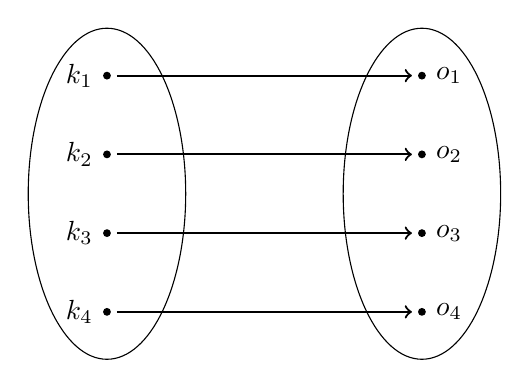
\begin{tikzpicture}[ele/.style={fill=black,circle,minimum width=.8pt,inner sep=1pt},every fit/.style={ellipse,draw,inner sep=-2pt}]
        \node[ele,label=left:{\normalsize	 $k_1$}] (a1) at (0,4) {};
        \node[ele,label=left:{\normalsize	 $k_2$}] (a2) at (0,3) {};
        \node[ele,label=left:{\normalsize	 $k_3$}] (a3) at (0,2) {};
        \node[ele,label=left:{\normalsize	 $k_4$}] (a4) at (0,1) {};

        \node[ele,,label=right:{\normalsize	 $o_1$}] (b1) at (4,4) {};
        \node[ele,,label=right:{\normalsize	 $o_2$}] (b2) at (4,3) {};
        \node[ele,,label=right:{\normalsize	 $o_3$}] (b3) at (4,2) {};
        \node[ele,,label=right:{\normalsize	 $o_4$}] (b4) at (4,1) {};

        \node[draw,fit= (a1) (a2) (a3) (a4),minimum width=2cm] {} ;
        \node[draw,fit= (b1) (b2) (b3) (b4),minimum width=2cm] {} ;
        \draw[->,thick,shorten <=2pt,shorten >=2pt] (a1) -- (b1);
        \draw[->,thick,shorten <=2pt,shorten >=2] (a2) -- (b2);
        \draw[->,thick,shorten <=2pt,shorten >=2] (a3) -- (b3);
        \draw[->,thick,shorten <=2pt,shorten >=2] (a4) -- (b4);
      \end{tikzpicture}
    }
    \caption*{(a) Noiseless Lossless}
  \end{minipage}
  \hfill
  \begin{minipage}{0.45\linewidth}
    \resizebox{\linewidth}{!}{

      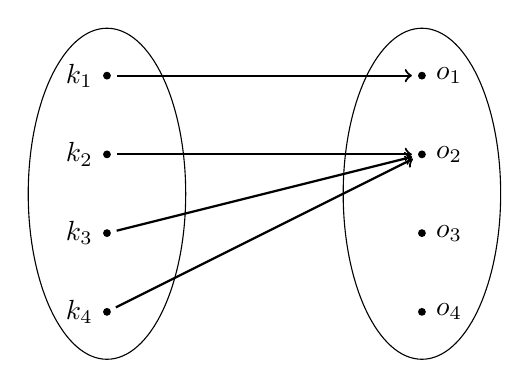
\begin{tikzpicture}[ele/.style={fill=black,circle,minimum width=.8pt,inner sep=1pt},every fit/.style={ellipse,draw,inner sep=-2pt}]
        \node[ele,label=left:{\normalsize $k_1$}] (a1) at (0,4) {};
        \node[ele,label=left:{\normalsize $k_2$}] (a2) at (0,3) {};
        \node[ele,label=left:{\normalsize $k_3$}] (a3) at (0,2) {};
        \node[ele,label=left:{\normalsize $k_4$}] (a4) at (0,1) {};

        \node[ele,,label=right:{\normalsize $o_1$}] (b1) at (4,4) {};
        \node[ele,,label=right:{\normalsize $o_2$}] (b2) at (4,3) {};
        \node[ele,,label=right:{\normalsize $o_3$}] (b3) at (4,2) {};
        \node[ele,,label=right:{\normalsize $o_4$}] (b4) at (4,1) {};

        \node[draw,fit= (a1) (a2) (a3) (a4),minimum width=2cm] {} ;
        \node[draw,fit= (b1) (b2) (b3) (b4),minimum width=2cm] {} ;
        \draw[->,thick,shorten <=2pt,shorten >=2pt] (a1) -- (b1);
        \draw[->,thick,shorten <=2pt,shorten >=2] (a2) -- (b2);
        \draw[->,thick,shorten <=2pt,shorten >=2] (a3) -- (b2);
        \draw[->,thick,shorten <=2pt,shorten >=2] (a4) -- (b2);
      \end{tikzpicture}
    }
    \caption*{(b) Noiseless Loss}
  \end{minipage}
  \caption{Two Kinds of Channels}\label{fig:channel}
\end{figure}


\subsubsection{Noiseless Loss Channel}
In reality, noiseless loss channel is more common. We define the channel is noiseless loss if

\begin{equation} \label{chapter:eq:5}
  C(K;O) = \max_{p(x)} I(K;O) = \max_{p(x)} H |O| = \log_2 {|O|}
\end{equation}

Figure~\ref{fig:channel}(b) shows the example of the type of the channel. Once the input symbol is determined, the output symbol is also determine. As we can see, the channel have the unique output ($o \in O$) for every input ($k \in K$).


\subsection{Threat Model and Math Notation}


We consider an attacker who shares the same hardware resource with the victim. The attacker may not know the memory access the victim program accesses directly, but he can infer whether some memory addresses are accessed or not at various granularities after \textit{each run} of the victim program. We call the memory access information as the observation ($O$) in the rest of the paper. This is a typical scenario for most side-channel attacks.  We also assume the attacker can have access to the source code of the victim program ($\beta$). It is a valid assumption since most side-channel attacks target open source software. Also like recent works, we assume the attacker have a noise-free observation. For some side-channel channels like the controlled-channel attacks, it is already true. The program ($\beta$) has $K$ as the sensitive input. $K$ is a finite set that consists of every possible keys ($k \in K$). The program also takes known messages $M$ as the input.

\begin{figure}[ht]
  \centering
  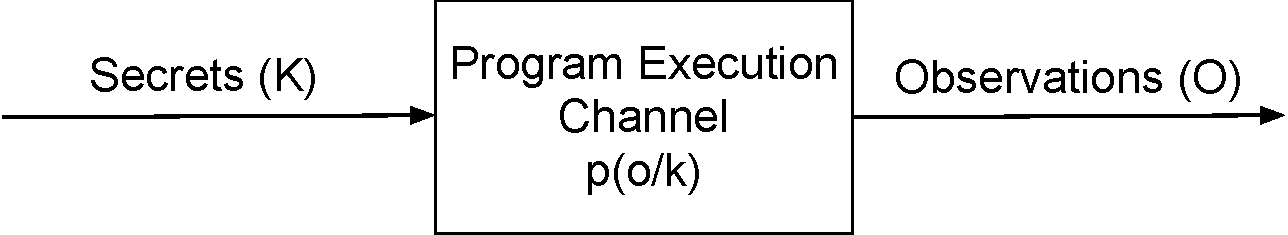
\includegraphics[width=.8\columnwidth]{./figures/chapter5/channel.pdf}
  \caption{The relationship between the side-channel attack and the channel capacity. For a deterministic program, the side-channel attack can be seen as the communication between the observation ($o \in O$) and the secret ($k \in K$) via a discrete memoryless channel.}
  \label{fig:side_channel}
\end{figure}

With the above definitions, we define the following mapping between $\beta$,
$K$, $M$, and $O$:

\begin{displaymath}
  \beta(K, M) \rightarrow O
\end{displaymath}


Side-channel attacks can be seen as a process that refers the secret ($K$) based on the observations ($O$) shown in the figure~\ref{fig:side_channel}. As an attacker, he can observe the memory address of the victim program. He wants to infer the original secret ($k$) based on the observation. We also assume the attacker knows the known message $m \in M$. In the rest of paper, we use $\beta(K) \rightarrow O$ to denote a victim program with side-channel vulnerabilities.


In this paper, we consider three types of granularity: byte (1 Byte), cache line size (64 Bytes), page size (4 KBs). To the best of our knowledge, the three types of granularities can cover most of the side-channel attacks in literature.

\section{Method}
In this section, we first provide two examples shows how we rank the side-channel vulnerability. After that, we prove that our method is the conservative estimate of the amount of the each leakage.

\subsection{An Example}
Figure~\ref{fig:example1} show a function that is vulnerable to side-channel attacks. The function take a input secret from the caller. Depending on the value of the secret, it may access different values at line 7. Suppose an attacker can observe which item in the table \textsf{T} is accessed, he can infer the secret based on the observation.
\begin{figure}[h]
  \begin{minipage}{0.6\linewidth}
    \begin{lstlisting}[xleftmargin=.15\textwidth,xrightmargin=.30\textwidth]
void bar(uint8_t secret)
{
  uint8_t T[128];
  uint8_t index = 0, t;
  int i;
  index = (index+secret)%128;
  t = T[index];
  ...
}
\end{lstlisting}
  \end{minipage}
  \hfill
  \begin{minipage}{0.4\linewidth}
    \resizebox{0.8\textwidth}{!}{%

      \begin{tabular}{cccccccccc}
        \toprule
        \diagbox{S}{T} & 0 & 1 & 2 & 3 & 4 & 5 & 6 & 7 & ... \\
        \midrule
        0              & A &   &   &   &   &                 \\
        1              &   & A &   &   &   &                 \\
        2              &   &   & A &   &   &                 \\
        3              &   &   &   & A &   &                 \\
        4              &   &   &   &   & A &                 \\
        5              &   &   &   &   &   & A &             \\
        6              &   &   &   &   &   &   & A           \\
        7              &   &   &   &   &   &   &   & A       \\
        \bottomrule
      \end{tabular}%
    }
  \end{minipage}
  \caption{A Serious Leakage.}\label{chapter5:fig:example1}
\end{figure}

To assess the sensitive level of the vulnerability, we use the sampling method to estimate the leakage. Suppose we give the function input from $0, 1, \dots, 7$ and observe the array $T$, we can find each different input have one unique observation. Therefore, the secret can be uniquely determined.

\begin{figure}[h]
  \begin{minipage}{0.60\linewidth}
    \begin{lstlisting}[xleftmargin=.15\textwidth,xrightmargin=.30\textwidth]
void bar(uint8_t secret)
{
  uint8_t T[128];
  uint8_t index = 0, t;
  int i;
  index = (index+secret)%128;
  t = T[index % 4];
  ...
}
\end{lstlisting}
  \end{minipage}
  \hfill
  \begin{minipage}{0.4\linewidth}
    \resizebox{0.8\textwidth}{!}{%

      \begin{tabular}{cccccccccc}
        \toprule
        \diagbox{S}{T} & 0 & 1 & 2 & 3 & 4 & 5 & 6 & 7 & ... \\
        \midrule
        0              & A &   &   &   &   &                 \\
        1              &   & A &   &   &   &                 \\
        2              &   &   & A &   &   &                 \\
        3              &   &   &   & A &   &                 \\
        4              & A &   &   &   &   &                 \\
        5              &   & A &   &   &   &   &             \\
        6              &   &   & A &   &   &   &             \\
        7              &   &   &   & A &   &   &   &         \\
        \bottomrule
      \end{tabular}%
    }
  \end{minipage}
  \caption{A Minor Leakage. }\label{chapter5:fig:example2}
\end{figure}
On the other hand, the second example also have a side-channel leakages at line 7. However, the leakage is slightly different. Still, we test the program with input from $0, 1, \dots, 7$. However, we find the attacker can not uniquely determine the secret based on the observation of table $T$. For example. both $0$ and $4$ read the first the item of the table. Therefore, we think the vulnerability is slightly minor than the previous one. Here comes with the definition of the amount of leaked information of the vulnerability.

\begin{mydef}
  \label{chapter5:def}
  Suppose we have a program $\beta$ with the input set $K$. We randomly select $k_1, k_2, \dots, k_n \in K' \subseteq K$ as the input. We denote it as
  $$\beta(K') \rightarrow	O'$$

  Here $O$ is a set that consists of various observations $o_1, o_2, \dots, o_m$. The amount of leaked information $L_{\beta(K')\rightarrow O'}$ based on the observation ($o$) is
  $$L_{\beta(K')\rightarrow O'} = H(O') $$
\end{mydef}


With Definition~\ref{chapter5:def}, we can calculate the information leakage in Figure~\ref{chapter5:fig:example1} and Figure~\ref{chapter5:fig:example2} respectively. In Figure~\ref{chapter5:fig:example1}, we have $8$ kinds of observations and each observation is uniformly distributed. Therefore, the information leakage is $log_2{8} = 3$ bits. In Figure~\ref{chapter5:fig:example2}, we have $4$ kinds of observations and each observation is also uniformly distributed. Therefore, the information leakage is $log_2{4} = 2$ bits. We test the program with $8$ inputs. Therefore, the Shannon entropy of the original K $H(K)$ is also $3\,\mathrm{bits}$. According to Equation~\ref{chapter5:eq1}. the secret-dependent data accesses in Figure~\ref{chapter5:fig:example1} can leak the sensitive information totally.

\subsection{A Conservative Estimation}
In this section, we prove Definition~\ref{chapter5:def} is the conservative estimation of the amount of leaked information based on the channel capacity.

\begin{theorem}\label{the1}
  If an attacker launches a side-channel attack on  deterministic programs, then the channel between the secret and the observation is a noiseless loss channel.
\end{theorem}

\begin{myprof}
  According to information theory,
  \begin{align*}
    I(K;O) & = H(O) - H(O|K)                                \\
           & = H(O) - \sum_{k {\in} K }{p(o|k)\log_2p(o|k)}
  \end{align*}
  For a deterministic program, $p(o|k)=1$. As a result, $H(O|K) = 0$.
  \begin{align*}
    C(K;O) = \max_{p(k)} I(K;O) = \max_{p(k)} H |O|
  \end{align*}
\end{myprof}

With THEOREM~\ref{the1}, we can have
\begin{align*}
  \max_{p(k)} H |O| >= \max_{p(k')} H |O'| >= H |O'|
\end{align*}

Accordingly, if Definition~\ref{chapter5:def} says the vulnerability leakage has $m$ bits of leakages, then the vulnerability can have at least $m$ bits of leakages. We can use the definition to detect those severe leakages. In the examples of Figure~\ref{chapter5:fig:example1} and Figure~\ref{chapter5:fig:example2}, because the input secret range from $0$ to $255$, we can calculate the precise value of the amount of information leakage by iterating each input keys. In Figure~\ref{chapter5:fig:example1}, each item in the array could be read. Therefore, the channel capacity in Figure~\ref{chapter5:fig:example1} is $\log_2{128} = \,7\, \mathrm{bits}$. In Figure~\ref{chapter5:fig:example2}, there could be $4$ kinds of information, so the information leakages defined by channel capacity is $\log_2{4} = \,2\, \mathrm{bits}$. Compared with the result from Definition~\ref{chapter5:def}, we can see that the amount of leakages by Definition is a conservative estimation.

\section{Align Address Access Across Multiple Executions}
We compare address accesses of different executions generated by different inputs to quantify the amount of leakage information. A meaningful comparison requires we align executions across multiple runs before we quantify the leakage. In this work, we combine the information from both the source code and the binary executable to align the memory access during the execution.


\begin{figure}[h]
  \begin{minipage}{0.45\linewidth}
    \begin{lstlisting}[numbers=none,xleftmargin=.1\textwidth,xrightmargin=.2\textwidth]
uint8_t *T = malloc(4);
if (T==NULL) exit(1);
...
t = T[i];    
\end{lstlisting}
  \end{minipage}
  \hfill
  \begin{minipage}{0.5\linewidth}
    \resizebox{\textwidth}{!}{

      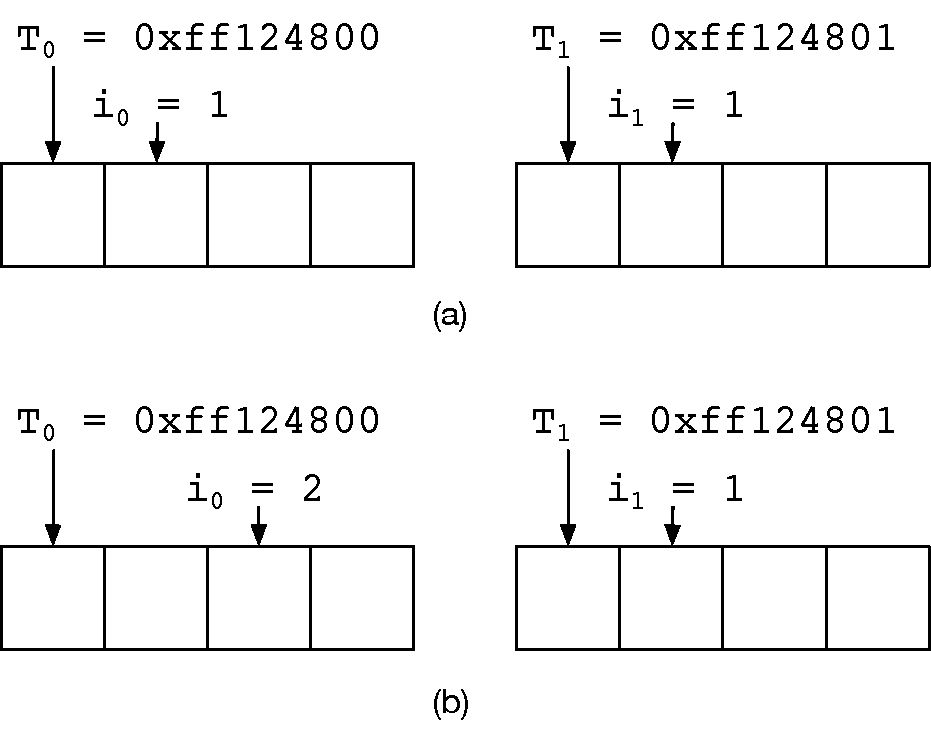
\includegraphics[width=\columnwidth]{./figures/chapter5/align.pdf}

    }
  \end{minipage}
  \caption{Without proper address alignment, there could be many false positives and false negatives.}\label{fig:align}
\end{figure}

Considering the example in figure~\ref{fig:align}, it read the data from the array \textsf{T} based on the index (i). If the index (i) is associated with a key, it could be a side-channel vulnerability. Unlike the example in the previous section, the array \textsf{T} is on the heap. Data on the heap are allocated in different addresses each time. Suppose during the first run, \textsf{T} is allocated at the address \textsf{0xff124800} and \textsf{T} is allocated at the address \textsf{0xff124801} at the second run. For the example in Figure~\ref{fig:align}(a), the index that used to access the array is always $1$, so it should not be a side-channel vulnerability here. However, because the based address is different. So we get two different memory accesses. Under the circumstance, it is a false positive. Besides, it can cause false negatives as the example shown in Figure~\ref{fig:align}(b). In the example, different keys lead to different index. However, as $T_0 + i_0$ equals to $T_1 + i_0$, \ can not observe the difference here, which can cause a false positive.

\textbf{Our Strategy: } We assign a value for each memory location~\cite{sumner2010memory}. The value should satisfy the following characteristics.
\begin{itemize}
  \item \textbf{Uniqueness.} At any point during the execution, different memory cells must have a different value.
  \item \textbf{Alignment.} The same memory cell across multiple executions should share the same value.
\end{itemize}

There are some possible solutions that can assign the value.
\textbf{Run-time Information.} One example here is the concrete memory address during the runtime. Such a value satisfy the uniqueness characteristic. However, as the example shown in Figure~\ref{fig:align}, it does not have the alignment property.
\textbf{Source Code Information.} Alternatively, we can use the information from the source code. Recent work~\cite{sumner2010memory} proposes using the execution point that allocate the memory cell as the index and tracking the pointer arithmetic to track the pointer that points to the memory. However, such a method may miss the alias symbol that points to the same memory cell.

We propose to combine both the information from the source code and the runtime to align the memory access during the execution. At the point the memory is allocated, we use the tuple $(start\ address, length)$ to represent the buffer. In the following execution, we check if any memory access falls into the range of those tuples. If so, we add the memory access into the tuple. After the execution, the tuple can be mapped into the location of the source code and we only compare the memory access that belongs to the same lines in the source code.

\section{Multiple Leakages Sites}
Real-world software can have many side-channel vulnerabilities. Those vulnerabilities may spread in the whole program. An adversary may exploit more than one side-channel vulnerabilities to gain more information~\cite{7163052, 191010}. In order to precisely quantify the
total information leakage, we need to know the relation of those leakage sites. 

\begin{figure}[h]
\begin{minipage}{0.4\linewidth}
\begin{lstlisting}
void function1(uint8_t* secret)
{
  uint8_t k1, k2;
  k1 = secret[1];
  k2 = secret[2];
  if (k1 > k2)
    a();
  if (k1 + k2 < 256)
    b();
  ...
}
\end{lstlisting}\caption*{(a) Independent Leakages}
\end{minipage}
\hfill
\begin{minipage}{0.4\linewidth}
\begin{lstlisting}
void function2(uint8_t* secret)
{
  uint8_t k1, k2;
  k1 = secret[1];
  k2 = secret[2];
  if (k1 + k2 > 128)
    c();
  if (k1 > 32)
    d();
  ...
}
\end{lstlisting} \caption*{(b) Dependent Leakages}
\end{minipage}
\caption{Multiple Leakages}\label{chapter5:fig:multiple}
\end{figure}

Considering the examples in Figure~\ref{chapter5:fig:multiple}, Figure~\ref{chapter5:fig:multiple}(a) show a code snippet with two leakage sites at line 6 and line 8 respectively. For example, if an adversary observes that function \textsf{a} executes, then the attacker can infer the first byte in buffer \textsf{secret} is larger than the second byte.  Similarly, if an adversary observes that function \textsf{b} executes, then the attacker can infer that the sum of the first two bytes in buffer \textsf{secret} is smaller than $256$. The interesting part here is that if the attacker observes that function \textsf{a} executes, then he still has zero knowledge about the function \textsf{b}. The two leakage sites in Figure~\ref{chapter5:fig:multiple}(b) are different. If an attacker observes function \textsf{c} executes, then it is likely the attacker can observe that function \textsf{d} also executes. 

Suppose one program has two side-channel vulnerabilities A and B, which can leak $L_A$ and $L_B$ bits respectively according to the definition~\ref{chapter5:def}. 
Depending on the relation between A and B, the total leaked information $L_{\mathit{total}}$ will be:

\subsection{Independent Leakages}
If A and B are independent leakages, the total information leakage will be:
\[L_{\mathit{total}} = L_A + L_B \]

\subsection{Dependent Leakages}
If A and B are dependent leakages, the total information leakage will be:
\[\max{\{L_A, L_B\}}  \leq L_{\mathit{total}} < L_A + L_B\]

We use the chi-square test to check if two leakage sites are independent. A chi-squared test can determine if there is a relationship between two categorical variables. Suppose we can summarize the data in a $r*c$  two-way contingency table. The chi-square test statistic and the degrees of freedom $v$ is calculated with the below formula:
\[\tilde{\chi}^2=\sum_{k=1}^{rc} \frac{(O_k - E_k)^2}{E_k}\] 
\[v = (r - 1)(c - 1)\]
Here $O$ is the observe value and $E$ is the expected value. A low value means that there is a high correlation between the two variables. 

The null hypothesis is that the two leakages are independent.
We generate random inputs as the secret and record the memory access for each execution. For each time, the execution is independent of the previous execution. The times of the same observation for each event should satisfy the normal distribution. After that, we can use the chi-squared test to test whether the two leakage sites are independent.

\begin{figure}[h]
  \begin{minipage}{0.40\linewidth}
      \begin{tabular}{rrrr}
        \toprule
        & $a$ & $\lnot a$  & total\\
        \midrule
        $b$   & 255 (255.5) & 253 (252.5) &   508  \\
        $\lnot b$   & 260 (259.5)  & 256 (256.5) &    516   \\
        total &   515 &  509   & 1,024   \\
        \bottomrule
      \end{tabular}\caption*{(a)}
  \end{minipage}
\hspace{-15pt}
\hfill
\hspace{-15pt}
  \begin{minipage}{0.40\linewidth}
      \begin{tabular}{rrrr}
        \toprule
        & $c$ & $\lnot c$  & total\\
        \midrule
        $d$   & 809 (764.8) & 82 (126.2) & 891    \\
        $\lnot d$   & 70 (114.2)  & 63 (18.8)&  133     \\
        total &  879 &  145  & 1,024    \\
        \bottomrule
      \end{tabular}\caption*{(b)}
  \end{minipage}
  \caption{The contingency table for the experiments. The numbers in the bracket are expected values. }\label{chapter5:fig:con_table}
\end{figure}


Assume we generate $1024$ random inputs and record the memory access each time. For the example in Figure~\ref{chapter5:fig:multiple}, we use $a$ to denote the function \textsf{a} executes and $\lnot a$ to denote the function \textsf{a} does not execute during the execution. After calculating the number of the same observation, we get the contingency table shown in Figure~\ref{chapter5:fig:con_table}. Suppose the observations of function \textsf{a} and function \textsf{b} are independent. We calculate the expected value for the observation $ab$ based on the frequency.
\[ E_{ab} = \frac{(255+256)*(255+253)}{1024} = 255.5\]
Similarly, we calculate the rest expected values with the hypothesis that the leakages are independent and fill in them in Figure~\ref{chapter5:fig:con_table}. The degree of freedom $v$ is $(2-1)*(2-1) = 1$.

Based on the equation, we calculate the chi-square test statistic for two leakage sites in Figure~\ref{chapter5:fig:multiple} (a) and (b).

\[\tilde{\chi}^2_{a}= \frac{(255.5-255)^2}{255.5} + \frac{(252.5-253)^2}{252.5} + \frac{(259.5-260)^2}{259.5} + \frac{(256.5-256)^2}{256.5} = 0.004\] 
\[\tilde{\chi}^2_{b}= \frac{(764.8-809)^2}{764.8} + \frac{(126.2-82)^2}{126.2} + \frac{(114.2-70)^2}{114.2} + \frac{(18.8-63)^2}{18.8} = 139.1\] 

According to Chi Square Distribution Table, we have the probability $p\approx0.95$ to accept the null hypothesis for the two leakages in Figure~\ref{chapter5:fig:multiple} (a). We have the probability $p\approx0.00$ to accept the null hypothesis for the two leakages in Figure~\ref{chapter5:fig:multiple} (b). Therefore, we infer that the two leakages in Figure~\ref{chapter5:fig:multiple} (a) are independent. And the two leakages Figure~\ref{chapter5:fig:multiple} (b) are dependent. In this paper, for any two leakage, if $p < 0.03$, we think the two leakage sites are independent. For each leakage points, we use the above method to test if any two leakage sites are independent. We combine them into a leakage are calculate the total amount of the leakage.
\section{Design}
In this section, we explain the implementation of \ctool{}.
we first present the overview of \ctool{}. After that, we discuss some design details to implement \ctool{}.

\subsection{Overview}
Figure~\ref{chapter5:fig:workflow} shows an overview of our side-channel leakages quantification tool. Given the source code of the victim program, \ctool{} can find the address-based side-channel leakages by fuzzing the victim program. To assist the illustration, we divide the workflow of ~\ctool{} into three steps. For the first step, we build the target program from the source code. After that, we give them random inputs to the victim program and run the target program and record each of the address in the binary file is hit or not and store the information in a bitmap. Next, we analyze the side-channel leakage from the address access bitmap. We split the address space into several segments to speed up the comparison according to Meta information. Finally, \ctool{} Generate the final leakage report. For each leakage sites, \ctool{} gives the conservative estimation of the information leakage. Every leakage site in the report is a true leakage and there is no false positives.

\begin{figure}[ht]
  \centering
  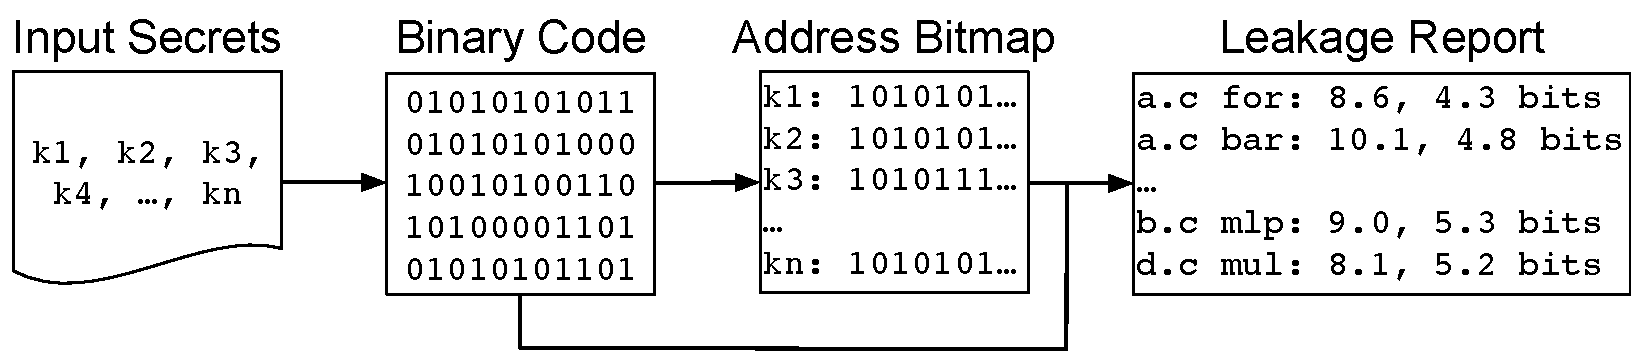
\includegraphics[width=\columnwidth]{./figures/chapter5/workflow.pdf}
  \caption{The workflow of \ctool{}. We try to divide the \ctool{} into three steps to assist the illustration. }\label{chapter5:fig:workflow}
\end{figure}

\subsection{Step 1: Fuzzing}
After we build the software into the binary executable, we give the binary code the random inputs. For cryptography libraries, the input is the encryption key. For non-cryptography libraries, the input could be images, text, and information in other format. Encryption algorithms like AES, DES take an array representing the secrets. We generate the random input by flipping the each bit of the keys. Some other programs also takes an buffer as the input. The buffer may contains the redundancy information and follow a specific format. So not any input that satisfies the input length is a valid input. Under the circumstance, we have a dictionary that contains the input. For example, Crypto libraries usually take PKCS \#1 as the input of RSA private key. We use some other tools to generate a list of valid keys and use the key to sample the program. Due to the enormous search space, we can not iterate every inputs. However, our method can give the conservative  estimate of each leakage site.
\subsection{Step 2: Address Record}
Next, we record the memory access information based on the input secret. We use the dynamic binary instrumentation (DBI) tool to record the whether a particular memory access information is accessed or not. Inspired by the AFL and valgrind, we use the bitmap to represent whether a particular memory is accessed or not. For example, the bitmap ${0101}$ of address $address_1, address_2, address_3, address_4$ means that $address_2, address_4$ are hit during the execution. During the execution, the direct information we get is the virtual memory address (VMA). However, we transfer the address into the offset (Load Memory Address (LMA)) in the original binary file. It has two benefits. First, modern computer systems employ the the Address Space Layout Randomization (ASLR). With ASLR, the operating system randomly put the enclave code and data at various memory offset. As a result, even for the same input, the code will get different execution traces because the enclave image is loaded at a different address each time Second, it helps us find the leakage site in the source code.

We rely on the program header and symbol information to recover the offset in the binary. During the loading process, the operating system maps each segment into a continuous memory region. So the offset of the virtual memory address between the code within the same segment is the same as the offset within the binary file. We choose the start address of some common functions (e.g, $main$) ($b$) as the navigation function. We get the virtual memory address of the start of the function ($\mathit{VMA_b}$) from the DBI tool and the load memory address of the function ($\mathit{LMA_b}$) from the symbol information. For any virtual address, we use Equation~\ref{equ:eq6} to calculate the offset in the original address.
\begin{equation}\label{equ:eq6}
  \mathit{LMA_a} = \mathit{LMA_b} - VMA_b - VMA_a
\end{equation}

There are two kinds of memory access: the access to the code and the access to the data.
\begin{itemize}
  \item Code Access. The memory address of the code is the value of $rip$ register. However, the length of x86 instructions can be from 1 byte to 15 bytes. For instructions whose length is longer than one byte, we also update the address  after the value $rip$ until the address reach the boundary of the instruction.
  \item Data Access. For instructions with memory access, we identify all the operands of each instruction and. Same as the code address, the instruction can read or write multiple bytes one time.  Instructions like \textsf{push} and \textsf{pop} have implicit memory access. We all update the bitmap of the address correspondingly.
\end{itemize}

\subsection{Step 3: Leakages Detection and Quantification}
In this step, we detect and quantify the side-channel leakage. For each $k \in K$, we have a boolean number ($0$ or $1$) to describe whether the address $addr$ is accessed or not during the execution when the input is $k$. For the brevity of description, For the brevity of description, we use $B^{addr}_{k_i}$ to denote the boolean number.



\subsubsection{Various Granularities Side-channel Detection}
\ctool{} can detect the side-channel vulnerabilities in different granularity. For each granularity, we calculate a new bitmap that represents access information of each unit. We have the bitmap of the memory access at the byte level. An attacker who has the coarse-grained observation at address space may not be able to distinguish the address difference. For example, modern X64 computer system uses 48-bit virtual memory addresses. The top 36 bit of the virtual address is called Virtual Page Number (VPN) and the bottom 12 bits of the virtual address is called offset. The memory management unit (MMU) transfer the virtual address into the physical address by mapping the Virtual Page Number (VPN) into the Physical Page Number (PPN) while keep the offset of the address. So two addresses with the Same VPN but different offset are not distinguishable by an attacker who only has the the page-level observation.

Suppose a program reads one byte at memory $\mathsf{0x7ffff7ffd001}$ when the secret is $k_1$ and reads a different byte at memory $\mathsf{0x7ffff7ffda01}$ when the secret is $k_2$, an attacker who has the page-level observation can not launch the attack but an attacker who launches the cache attack can know the input is $k_1$ or $k_2$. We update the new bitmap of the large unit by merging the bitmaps of small units that fall into the large unit. That is, $\forall addr_1, addr_2, \dots, addr_n \in addr_N, B^{addr_N}_{k_i} = B^{addr_1}_{k_i} \lor,\dots,\lor B^{addr_N}_{k_n}$.


\subsubsection{Leakage Detection} The access of the address is secret-dependent if $ \exists\, k_{i1}, k_{i2} \in K, \, B^{addr}_{k_i1} \oplus  B^{addr}_{k_i2} =1 $. In the paper, we perform the logical exclusive OR operation on every boolearn value in the same address. If the result is $1$, then the address is vulnerable to the side-channel attacks.

\begin{myexample}
Suppose we sample a program from $k1$ to $k8$ and record the memory access at the granularity of each byte from $\mathsf{7ffff7ffd000}$ to $\mathsf{7ffff7ffd03f}$ (One cache line), we perform the bit-wise or operation of each address with the address range. Because the cache line is always accessed. We think it is not a leak here.
\begin{center}
  \begin{tabular}{c}
    {
      \begin{lstlisting}[frame=none]
              k1  k2  k3  k4  k5  k6  k7  k8   Result  
7ffff7ffd000   1   0   1   0   1   1   0   1 
7ffff7ffd000   0   1   1   0   1   1   1   1 
7ffff7ffd000   1   1   1   1   1   1   0   1 
7ffff7ffd000   1   0   1   0   1   1   1   1 
...
7ffff7ffd03f   1   0   1   0   1   1   1   0  
cache line     1   1   1   1   1   1   1   1    0 (No Leaks)
\end{lstlisting}
    }
  \end{tabular}
\end{center}
\end{myexample}

\subsubsection{Estimate The Leaked Information}
According to Definition~\ref{chapter5:def}, we quantify the information leakage based on the distribution of the observation. If we calculate the information leakage from an $4MB$ memory area, then the length of the byte-level bitmap is $4*1024*1024 = 4194304$. While it is possible to compute the distribution of the bitmap theoretically, it is hard to compare the bitmap of such length in practice.

To solve the problem, we use the debug information to split the bitmap into several segments and map the leakage site into the location of the source code. Each segment maps the address access situation of the function in the source code. In our setting, the max length of the bitmap of each segment is $1024$, the length of \textsf{uint1024\_t}. So we can put the bitmap into a variable. The split operation ease the computation. But it also adds the limitation of max address range when we quantify the side-channel leakage shown in Table~\ref{tab:size_limitation}. We think the range of the memory is big enough for us to quantify the most of the cache side-channel attacks.

\begin{table}[h]
  \centering
  \resizebox{0.8\textwidth}{!}{%

    \begin{tabular}{llll}
      \toprule
      Granularity & Byte       & Cache Line (64 Bytes) & Memory Page (4 KB) \\
      \midrule
      Range       & 1024 Bytes & 64 KB                 & 4 KB               \\
      \bottomrule
    \end{tabular}
  }
  \caption{The maximum range address range when we quantify the amount of the leakage with different granularity.}
  \label{tab:size_limitation}
\end{table}

After that, we traverse the bitmap for each $k$ and count it to get the distribution of the bitmap. The counting process is like traversing a binary tree.

\begin{myexample}
Shown in Figure~\ref{fig:design:example2}, we have the following observation from $k_1$ to $k_8$, then we count the distribution of  the observation. The process is like traversing a binary tree and increase the counter of the child node. According to Definition~\ref{chapter5:def}, the amount of the leakage is

\begin{displaymath}
  H(O') = - \frac{3}{8}*\log_2{\frac{3}{8}}- \frac{1}{2}*\log_2{\frac{1}{2}}
  - \frac{1}{8}*\log_2{\frac{1}{8}} = 1.4 \,\mathrm{bits}
\end{displaymath}

\begin{figure}[h]
  \begin{minipage}{0.3\linewidth}
    \resizebox{\linewidth}{!}{
      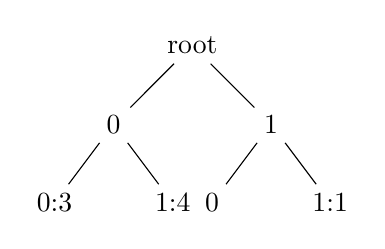
\begin{tikzpicture}
        [level distance=1cm,
          level 1/.style={sibling distance=2cm},
          level 2/.style={sibling distance=1.5cm}]
        \node {root}
        child {node {0}
            child {node {0:3}}
            child {node {1:4}}
          }
        child {node {1}
            child {node {0}}
            child {node {1:1}}
          };
      \end{tikzpicture}

    }\end{minipage}
  \hfill
  \begin{minipage}{0.2\linewidth}
    {
      \begin{lstlisting}[frame=none, numbers=none]
k1  00
k2  01
k3  01
k4  01
k5  00
k6  01
k7  11
k8  00
\end{lstlisting}
    }
  \end{minipage}
  \hfill
  \begin{minipage}{0.25\linewidth}
    \resizebox{\linewidth}{!}{

      \begin{tabular}{ll}
        \toprule
        Observation & P     \\
        \midrule
        00          & $3/8$ \\
        01          & $1/2$ \\
        10          & 0     \\
        11          & $1/8$ \\
        \bottomrule
      \end{tabular}
    }
  \end{minipage}
  \caption{Example 2}\label{fig:design:example2}
\end{figure}
\end{myexample}


\section{Implementation}
We have implemented a prototype of \ctool{}. It takes an input of ELF binary as well as the source code of the corresponding problem. The front-end of \ctool{} is implemented in Python. It can generate random inputs and test the program with those inputs many times.  The address record part is implemented as an Intel Pin tool plugin in C++ to record the bitmap for each input. The main component uses \textsf{libelfin}, an open source library to parse ELF binaries and read DWARF debug information. The current implementation can support  64-bits ELF binary in Linux. 

\section{Evaluation}
In this section, we evaluate \ctool{} on several small benchmarks and real-world software trying to answer the following questions:

\begin{itemize}
\item \textbf{Effectiveness:} Can \ctool{} quantify the information leakage with an conservative estimation? If so, what is the loss compared it with the real leakage?
\item \textbf{Performance:} What are overhead costs of \ctool{}?
\item \textbf{Usage:}  Can \ctool{} help developers find and fix side-channel leakages?
\end{itemize}

\textbf{Evaluation setup.} We run all the following experiment in a machine with Ubuntu 18.04 LTS. The server machine equips with 2.30GHz Intel Core i9-9880 CPU with 16GB RAM memory. We use the default release settings to build the source code of the software into ELF 64-bit executables with GCC 7.5. 

\textbf{Benchmarks.} 
We collect benchmarks from real-world applications and libraries. Our test programs cover applications from diverse functionalities, including small programs, cryptography, machine learning applications, and graphic libraries. 

\textit{Small Programs:} We use two benchmarks that are well studied in the previous work. The amount of actual leakage of those samples are known. We use them to evaluate the precision of the tool.

\textit{Cryptography Applications:} Our benchmarks include the most popular cryptography libraries, such as mebdTLS, OpenSSL, Libgcropt, and wolfSSL. Encryption ciphers can be divided into three categories:  symmetric ciphers, and asymmetric ciphers. For stream ciphers, we use RC4. For symmetric ciphers, we choose AES. We also evaluate the tool on RSA, a widely used algorithm in the public-key cryptosystem.

\textit{Machine Learning Applications:} We evaluate the tool on TinyDNN, a dependency-free deep learning framework in C++.

\textit{Graphic Libraries:} We evaluate the tool on GTK, a popular graphic library. Previous research has demonstrated attacks to infer the keystroke.

\begin{table}
\footnotesize
\caption{Evaluation results overview: Name of the benchmark, The Size of the Input Data, The number of leaked functions, The Maximum Leakage, The size of the benchmark, and The Performance.}\label{chapter5:table:over_result}
\centering
\resizebox{\columnwidth}{!}{
\begin{tabular}{lrrrrrrrrrrr}\toprule

\textbf{Benchmark}   & \multicolumn{2}{c}{\textbf{Input Data}} &  \multicolumn{2}{c}{\textbf{\# Leaked Functions}} & \multicolumn{2}{c}{\textbf{Max. Leak (bits)}}   & \multicolumn{2}{c}{\textbf{Program Size}}    & \multicolumn{3}{c}{\textbf{Performance}}    \\ 
\cmidrule(lr){2-3}\cmidrule(lr){4-5}\cmidrule(lr){6-7}\cmidrule(lr){8-9}\cmidrule(lr){10-12}& \# & bits &  1 Byte &  64 Bytes & 1 Byte  & 64 Bytes & LoC & Size & Fuzzing & Comparison & Chi-squared
\\\midrule
Unsafe Password Checker& 4096& 12.0& 1&0&0.04&  0& 18 & 104 KB & 2.4 min & 0.4 min & 0 min\\
Safe Password Checker & 4096 & 12.0& 0&0 &0 &0 & 20 & 106 KB & 2.3 min & 0.4 min & 0 min\\
One-byte Lookup Table & 4096 & 12.0& 1&1&7.5& 3.6 & 18 & 104 KB & 0.8 min & 0.1 min & 0 min\\
Four-byte Lookup Table & 4096 & 12.0& 1&1&9.6& 8.5 & 18 & 104 KB & 0.7 min & 0.1 min & 0 min\\
AES T-Table mbedTLS 2.15 & 4096 & 12.0&2&2&11.6 &6.7& -& 1.1 MB &4.1 min & 0.8 min & 0.1 min  \\
AES NI mbedTLS 2.15 & 4096 & 12.0&0&0&0 &0&-& 1.1 MB & 2.8 min & 0 min & 0 min  \\
AES OpenSSL 1.1.0  & 4096 & 12.0 & 1&0 &1.4 & 0&-& 1.0 MB  & 3.1 min & 0.2 min & 0 min \\
AES  OpenSSL 1.1.1& 4096 & 12.0 & 1&0 &1.3&0&-& 909 KB & 2.9 min & 0.2 min & 0 min\\
AES  wolfSSL 4.5.0& 4096 & 12.0 &1&0& 0.11& 0 & - &1.1 MB & 3.3 min & 0.1 min & 0 min \\
AES Libgcrypt 1.8.7& 4096 & 12.0 &0 &0 &0&0 &-&4.4 MB & 10.2 min& 0 min & 0 min\\
RSA mbedTLS 2.15& 4096 & 12.0 &10&8&13.3& 6.0 &-&1.8 MB& 1321.1 min & 63.5 min & 5.1 min \\
RSA OpenSSL 1.1.0& 4096 & 12.0 &14&6&8.7& 6.1 &-& 11 MB & 981.1 min & 75.4 min & 4.5 min\\
RSA OpenSSL 1.1.1& 4096 & 12.0 &6&4&6.3& 2.1&-&13 MB & 1021.1 min & 45.1 min & 5.5 min\\
RSA wolfSSL 4.5.0& 4096 & 12.0 &5&2&3.4& 2.5&-&4.2 MB & 1613.6 min & 51.6 min & 7.9 min\\
RSA Libgcrypt 1.8.7& 4096 & 12.0 &8&6&8.6& 6.6&-&4.4 MB & 1412.6 min & 23.9 min & 4.3 min\\
Tiny DNN & 12000 & - & 17&14&17.1&16.1&-& 4.4 MB & 183.5 min & 24.6 min & 5.2 min\\
GDK 3.24.23 & 4096 & 16.0 & 33&31& 12.1& 6.0&-& 48.5 MB & 60.8 min & 4.1 min & 1.5 min\\
\bottomrule
\end{tabular}
}

\end{table}

Table~\ref{chapter5:table:over_result} presents the overview result. The minimum unit of the program during the experiment is the function. Suppose the function has more than one access map, then the function that is vulnerable to side-channel attacks. We measure the side-channel leakages at two different granularities: the byte level and the cache line level. The result shows that the program has more leaked vulnerabilities and tends to leak more information at the byte level compare with the cache line level. Each time we run the target program under random inputs and record memory accesses. For cryptography programs, we run the target program with $4096$ different inputs. During the fuzzing process, if the program does not have new memory access bitmap after several rounds. We call the fuzzing step is fixed. From the side-channel detection aspect, it is not necessary to continue running the experiments since more rounds do not reveal new leakages. During the experiment, we find AES ciphers reach the fixed point after about 300 rounds and RSA can reach the fixed point after around 500 rounds. Previous work~\cite{217537} also reported similar result. During our experiment, we continue running the experiment until the observe value for the same observation is at least 5 to satisfy the Chi-square test requirement. Therefore, we choose to run all the cipher with different inputs for $4096$ times.  If one program has more than two leaked functions, we run the chi-squared test and calculate the total amount of leakages.

\subsection{Benchmarks}
\subsubsection{Password Checker}
\begin{figure}
  \begin{minipage}{0.45\linewidth}
    \begin{lstlisting}[xleftmargin=.0\textwidth, xrightmargin=.0\textwidth, frame=none]
bool pwcheck(uint8_t *key, uint8_t *pub) {
  for (int i = 0; i < 2; ++i) {
    if (key[i] != pub[i]) {
      return false;
    }
  }
  return true;
}
\end{lstlisting}
  \end{minipage}
  \hfill
  \begin{minipage}{0.45\linewidth}
    \begin{lstlisting}[xleftmargin=.0\textwidth, xrightmargin=.00\textwidth, frame=none]
bool pwcheck(uint8_t *key, uint8_t *pub) {
  bool matched = true;
  for (int i = 0; i < 2; ++i) {
    if (pub[i] != key[i]) 
      matched = false;
  }
  return matched;
}
\end{lstlisting}
  \end{minipage}
  \caption{A password checker. The left version is vulnerable to side-channel attacks. The right version is the fixed version.}\label{fig:chapter5:pwcheck}
\end{figure}

We illustrate the quantification method on a password checking example.  As shown in Figure~\label{fig:chapter5:pwcheck}, the left version is vulnerable to side-channel attacks because of the early return at line 4. If the first bytes of \textsf{key} and \textsf{pub} are the same, the function will continue running and access the second byte. The right version fixes the vulnerability because the function will continue comparing the second byte even if the first byte is different.  \ctool{} identifies the leakage site in the left figure successfully and estimates the amount of leakage site is $0.04$ bits. 


\subsubsection{Lookup Table}
\begin{figure}
\centering
    \begin{lstlisting}[xleftmargin=.1\textwidth, xrightmargin=.1\textwidth, frame=none]
static const uint8_t T[1024] = {
      0x63U, 0x7cU, 0x77U, 0x7bU, 0xf2U, 0x6bU, 0x6fU, 0xc5U,
      0x30U, 0x01U, 0x67U, 0x2bU, 0xfeU, 0xd7U, 0xabU, 0x76U,
...
output = (T[(key[0]>>24)] << 24) ^
         (T[(key[1]>>16) & 0xff] << 16) ^
         (T[(key[2]>>8) & 0xff] << 8) ^
         (T[(key[3]) & 0xff]);
\end{lstlisting}
  \caption{Lookup Tables with Small Entries.}\label{fig:chapter5:small_lookup}
\end{figure}

\begin{figure}
\centering
    \begin{lstlisting}[xleftmargin=.1\textwidth, xrightmargin=.1\textwidth, frame=none]
static const uint32_t T[256] = {
    0xc66363a5U, 0xf87c7c84U, 0xee777799U, 0xf67b7b8dU,
    0xfff2f20dU, 0xd66b6bbdU, 0xde6f6fb1U, 0x91c5c554U,
    0x60303050U, 0x02010103U, 0xce6767a9U, 0x562b2b7dU,
    0xe7fefe19U, 0xb5d7d762U, 0x4dababe6U, 0xec76769aU};
...
output = (T[(key[0]>>24)] << 24) ^
         (T[(key[1]>>16) & 0xff] << 16) ^
         (T[(key[2]>>8) & 0xff] << 8) ^
         (T[(key[3]) & 0xff]);
\end{lstlisting}
  \caption{Lookup Tables with Big Entries.}\label{fig:chapter5:big_lookup}
\end{figure}

We analyze the table lookup with \ctool{}. It is a common operation used by symmetric ciphers like AES. Figure~\ref{fig:chapter5:big_lookup} is from the original AES reference implementation. It uses a lookup table and each entry is 4 bytes, which is vulnerable to side-channel attacks. Most cryptography libraries adopted the mitigated version, shown in Figure~\ref{fig:chapter5:small_lookup}. The evaluation result shows the version with smaller lookup tables leaks less information, which confirm the effectiveness of the mitigation technique.

\subsection{Cryptography Libraries}
AES encryption can be divided into three steps. In the first step, the round keys are derived from the encryption keys called the AES key schedule, and the state array is initialized with the plain-text and the initial round step. In the second step, the AES performs eleven rounds of state manipulation. In the final stage, the state array is copied out as the encrypted data.
The reference implementation uses lookup tables in the first two steps. Intuitively, the implementation is vulnerable to side-channel attacks. There are some mitigated versions of AES. We evaluate \ctool{} on three variants of AES implementations: the reference implementation, the bit-sliced version, and the AES-NI implementation.
For mebedTLS, we evaluate AES-NI and the reference implementation. We do not find any leakage sites in the AES-NI version. On the other hand, the reference implementation has several leakage sites. The bit-sliced version from OpenSSL and wolfSSL should be resistant to side-channel attacks. However, we find they only adopt the protection in the encryption function but leave the key expansion function unprotected. The T-Table implementation has side-channel leakage sites in both the key expanding function and the actually encryption function. 

We use a fixed RSA blinding value to avoid non-deterministic behaviors during the execution. After that, we compare the result with the previous work~\cite{bao2021abacus,203878}. The result shows that \ctool{} can identify all the leakage sites reported in the previous work. In addition, \ctool{} identify new leakages in the private key decoded functions (\textsf{EVP\_DecodeUpdate}, \textsf{EVP\_DecodeBlock}) in OpenSSL 1.1.0f.  To evaluate the effectiveness of the quantification result, we compare the RSA implementation between OpenSSL 1.1.0 and OpenSSL 1.1.1. Table~\ref{chapter5:tab:RSAOpenSSL1.1.0} shows the summary. Note that \ctool{} can analyze the side-channel leakages at both the byte granularity and the cache line granularity. However, we only show the result in cache line granularity. We compare the result with \tool{}, a symbolic analysis based side-channel quantification tool. \tool{} can tell which line actually leaks the information. So it is possible that one function has several two leakage sites. 

\begin{table}[!ht]
\centering\tiny\scriptsize
\caption{Leaked Functions in RSA implemented by OpenSSL 1.1.0}\label{chapter5:tab:RSAOpenSSL1.1.0}
%\resizebox{\columnwidth}{!}{
\begin{tabular}{llrrc}
\hline
\textbf{File}  & \textbf{Function} & \textbf{\tool{} Result} & \textbf{\ctool{} Result} & \textbf{Fixed in OpenSSL 1.1.1} \\\hline
bn\_lib.c& BN\_num\_bits\_word&*&CF & \cmark\\
bn\_lib.c& bn\_correct\_top&*&CF\\
bn\_lib.c& BN\_ucmp&*&CF\\
ct\_b64.c& \_\_udivdi3&5.9 &CF\\
bn\_div.c& BN\_div&*&CF\\
bn\_gcd.c& int\_bn\_mod\_inverse&1.0 &CF\\
bn\_lib.c& BN\_num\_bits\_word&*&DA\\
bn\_div.c& BN\_div&17.2 &CF\\
bn\_exp.c& BN\_mod\_exp\_mont\_consttime&1.0 &CF\\
bn\_mont.c& BN\_from\_montgomery\_word&*&DA\\
bn\_asm.c& bn\_sqr\_comba8&*&CF\\
bn\_mont.c& BN\_from\_montgomery\_word&0.0 &CF\\
bn\_div.c& BN\_div&0.3 &CF\\
\hline
\end{tabular}
%}
\renewcommand{\baselinestretch}{1.0}\selectfont
\end{table}
\subsection{Machine Learning Applications}
In the section, we demonstrate an attack that can recover the deep learning model inference output by the controlled-channel attack. Running the machine learning inference engine inside the enclave is a typical scenario for machine learning as service. The machine learning service provider upload the the trained model into an enclave running on the cloud platform and provide machine learning service to a third party user. With the help of the enclave, both the model and the user's inferred result is protected from the outside. However, we will show that the above information can be easily retrieved from the untrusted world through the side-channel attack.

We use MNIST as the dataset and LeNet-5 for MNIST digits recognition task. LeNet-5 is known to work well on handwritten digit recognition. We first train the network. The batch size in our experiment is 10 and the numbers of epochs is 30. After the training, the accuracy of the neural networks on test set images is 99.5\%. Then we use the model to infer the images. During the inference, we also record the page access information. 



\section{Discussion}

This paper presents an approach that tries to give the conservative estimate of the amount of leaked information by address-based side-channel attacks. Those attacks exploit the data-flow from secrets to load address and the data-flow from the data-flow from secrets to branch conditions to retrieve secrets based on the observation on the memory accesses. Despite those kinds of side-channel leakages have been discovered for decades, the up-to-date software still has some side channel leakages. For some of those vulnerabilities, developers don't fix them because they think those side-channel vulnerabilities are not important. To show the importance of those side-channel leakages, one way is to demonstrate an end-to-end attack based on the vulnerability. However, demonstrating an end-to-end attack often need a lots of manual efforts and the domain knowledge of the victim program, which is not often the case in practices. It is good to have a tool that can assess the severity level of those side channel leakages automatically. So it would be better to have a proper metric to quantify the side-channel leakage. However, we find previous side-channel quantification tools are developed to  ensure the noninterference of the program. They use over approximation heuristics method to quantify the leakage. For example, CacheAudit estimates that a 128-bit AES encryption can leaks more than 128 bits. As a result, even those tool reports severe leakage, it does not mean the program has a truly severe leakage.

Our tool can give the conservative estimation of the side-channel leakage based on Channel Capacity. The channel capacity measures  the information flow between the source and the destination. One useful characteristic of channel capacity is not affected by the distribution of the input, which is useful because in practice we can not have an assumption on the input secrets of the software. In the paper, we use the sampling result to over approximate the true value of the channel capacity. We prove the sampling method presented in the paper can only give the conservative estimation of the amount of the true leakage.

\ctool{} is a dynamic approach. So it bears the same limitations of dynamic approaches as well. \ctool{} may have the coverage problem and can miss some side-channel vulnerabilities. It is usually not a crucial problem for cryptography libraries as cryptography libraries are designed to have the same control-flow with various inputs. For other libraries like graphic rendering, machine learning, \ctool{} is very likely to miss some side-channel vulnerabilities. However, \ctool{} is not designed to find side-channel vulnerabilities. The goal of \ctool{} is to pick up those really serious side-channel vulnerabilities from the numerous vulnerabilities. So we do not think it is a main limitation of \ctool{}. However, users of \ctool{} should be aware the code coverage problem.

\begin{figure}
  \centering
  \begin{lstlisting}[xleftmargin=.2\textwidth, xrightmargin=.2\textwidth]
int foo(uint8_t secret){
  uint8_t index = 0, t;
  index = (index+secret)%128; // The index contains secrets
  ...
  if(index == 0){             // Secret-dependent flows
    bar(r, x, n)              // The observation
  }
  ...
}
\end{lstlisting}
  \caption{A code fragment}
  \label{fig:limitation}
\end{figure}


Another limitation is that \ctool{} can only find the position in the code that leaks the sensitive information, but it is not the root cause of the leaks. Consider the example in Figure~\ref{fig:limitation}, it takes the secret as the input. At line 3, it calculate an index based on the value of the secret. Depending on the value of index, it may or may not run the code at line 6. So line 5 is the reason that causes the vulnerability. But \ctool{} can only tell the line 6 can leak the information, despite it is not the root cause of the vulnerability.



\chapter{Discussion and Limitations}\label{chapter6}
\section{Fast and Precise Side-channel Vulnerability Detection}
\subsection*{Code Coverage} \detect{} analyzes one native x86 execution trace each time. The design, which is very precise in terms of true leakages compared to many static source code methods~\cite{197207,BacelarAlmeida:2013:FVS:2483313.2483334}, share common limitations of dynamic approaches. \detect{} may only cover part of the code. Each time we only get one single execution trace. Therefore, we may neglect some side-channel vulnerabilities not covered by the traces analyzed. However, this is not a crucial problem for analyzing cryptographic libraries, because cryptographic libraries are designed to have the same code coverage under various inputs. The evaluation result also confirms the above intuition. For symmetric encryption, there is no secret-dependent control-flow transfers during our evaluation. RSA implementations have several secret-dependent control-flow transfers. Many of them are bound checks, which do not leak much information and have negligible effects on the whole code coverage as well.

\subsection*{Design Choices} At the early stage of the project, we use SMT solvers to get the solutions of constraints. However, we find for some ciphers (RSA), \detect{} times out after several days. The profiling result shows that the tool spends most its time in Z3. Later, we use a sampling method to detect side-channel leakages. The sampling method seems simple and may miss some leakages in theory. However, the evaluation result shows \detect{} can identify all leakages found by the previous work~\cite{203878,236338,Brotzman19Casym}.  

\subsection*{Cache Model} We use a simple cache model in this work. Recent work such as CaSym~\cite{Brotzman19Casym,182946} uses an LRU cache. First, there is no fundamental difficulties for us to adopt a more realistic cache models. Second, the LRU model is still a substantial simplification of a real cache. However, their choice of a logical model of cache can bring expensive overheads. As a result, CaSym can only analyze small code snippets.

\subsection*{Leakages} While recent works have reported lots of potential side-channel vulnerabilities, most of them are not patched by developers. The DES implementation of OpenSSL has a few side-channel leakages, but given the end life status of DES, it is still unpatched for the worth of engineering effort. \detect{} also detects several leakages in asymmetric ciphers such as RSA. After we manually analyze these leakage sites, we find many of them leak very little or useless information (e.g., the length of big numbers), which may partially explain why developers are not interested in fix all the side-channel leakages. 

\section{Precise Analysis on Single-trace Attacks}
While recent work found many side-channel vulnerabilities,
we note that many of them are been patched by developers.
Side-channels are ubiquitous in software, and it is difficult to fix all of them.
We need a tool that estimates the sensitivity of each vulnerability
so software engineers can focus on
``severe'' leakages. For example, \tool{} reports that
the modular exponentiation using square and multiply algorithms can
leak more information than a key validation function.

Software developers can use \tool{} to find severe vulnerabilities
and reason about countermeasures.
\tool{} estimates the amount of leaked information for each side-channel leakage
in one execution trace. \tool{} is useful for software
engineers to test programs and fix vulnerabilities.
The design, which is more precise in reporting true leakages as compared with other static
methods~\cite{197207,BacelarAlmeida:2013:FVS:2483313.2483334}, obviously misses leakages on unexplored traces. The amount of leaked information quantified by \tool{} also depends on the value of secret keys.
However, as the tool is intended for debugging and testing,
we think it is a software engineer's responsibility to select the input key and trigger
the path in which they are interested. It is not a problem for crypto software 
since virtually all keys follow similar computational paths.

We use the amount of leaked information to represent the sensitivity level of
each side-channel vulnerability. Although imperfect, \tool{} produces a reasonable
measurement for each leak. For example, the simple modular exponentiation is
notoriously famous for multiple side-channel attacks~\cite{kocher1996timing}.
During the execution, a single leak point may execute multiple times
and each time leak a different bit. In this case, \tool{} reports that the
vulnerability can leak the whole key. However, not every leak point inside a
loop is severe. If a site in the loop leaks the same bit from the
original key, and these leaks are not independent. \tool{} captures most
fine-grained information by modeling each leak during the execution as a
formula and the conjunction of the formulas to describe its total effect.
Some leakage sites (e.g., square and multiply)
can leak one particular bit of the original key, but some leakage sites leak one bit
from several bytes in the original key. \tool{} can capture the dependency among the leaks and
reports more precise leakage information.

\tool{} reaches full precision if the number of estimated leaked bits
equals to Definition~\ref{chapter4:def}.
\tool{} may lose precision from the
memory model it uses in theory. However, we did not find false positives
caused by the imprecise memory model during our evaluation.
Sampling introduces imprecision but with a probabilistic guarantee.
However, during the evaluation, we find that \tool{} cannot estimate
the amount of leakage for some leakage sites in a reasonable time,
which means the number of $K^o$ is very small. According to Definition~\ref{chapter4:def}, it means the leakage is very severe. 
\section{Precise Analysis on Multiple-trace Attacks}
This paper presents an approach that tries to give a conservative
estimate of the amount of leaked information by address-based
side-channel attacks. These attacks exploit the data-flow from secrets
to load address and the data-flow from the data-flow from secrets to
branch conditions to retrieve secrets based on the observation on the
memory accesses. Although these kinds of side-channel leakages have
been discovered for decades, the up-to-date software still has some
side-channel leakages. For some of these vulnerabilities, developers
do not fix them because they think these side-channel vulnerabilities
are not important. To show the importance of these side-channel
leakages, one way is to demonstrate an end-to-end attack based on the
vulnerability. However, demonstrating an end-to-end attack often need
a lot of manual effort and the domain knowledge of the victim program,
which is not often the case in practice. It is good to have a tool
that automatically assesses the severity level of these side-channel
leakages. So it would be better to have a proper metric to quantify
the side-channel leakage. However, we find previous side-channel
quantification tools are developed to ensure the noninterference of
the program. They use the over-approximation heuristics method to
quantify the leakage. For example, CacheAudit estimates that a 128-bit
AES encryption can leak more than 128 bits. As a result, even these
tools report severe leakage, it does not mean the program has a truly
severe leakage.

Our tool can give a conservative estimation of the
side-channel leakage based on Channel Capacity. The channel capacity
measures the information flow between the source and the
destination. One useful characteristic of channel capacity is not
affected by the input, which is useful because we cannot
assume the input secrets of the software in practice. In the paper, we
use the sampling result to approximate the true value of the
channel capacity. We prove the sampling method presented in the paper can only give the conservative estimation of the amount of the true leakage.

\ctool{} requires the random input variables to be independent and identically distributed (i.i.d.). That's why I apply a black box fuzzing instead of a coverage-guided fuzzing. As long as each time we get a random input from the whole input space (Population) that is independent of the previous input, the input variables should satisfy the i.i.d. assumption. For AES-128 encryption, each time we randomly generate a 128 bit key from $0$ to $2^{128}$, the sequence of key values follows the i.i.d. assumption. The situation is a little different for machine learning libraries. In the dissertation, we evaluated \ctool{} on a deep learning model. Each time, we randomly select an item from a dataset (Sample). If the dataset is biased, then we can not get correct results. The good news is that the most well-known data set in machine learning is i.i.d.. i.i.d. is the foundation of supervised machine learning algorithms. In my dissertation, we used MINIST, a well-known handwriting dataset. The dataset is widely used in many supervised machine learning tasks.  We believe the i.i.d. assumption holds under the circumstance.

\ctool{} is a dynamic approach. So it bears the same limitations of dynamic approaches as well. \ctool{} may have the coverage problem and can miss some side-channel vulnerabilities. It is usually not a crucial problem for cryptography libraries as cryptography libraries are designed to have the same control flow under various inputs. For other libraries such as graphic rendering, machine learning, \ctool{} is very likely to miss some side-channel vulnerabilities. However, \ctool{} is not designed to find side-channel vulnerabilities. The goal of \ctool{} is to pick up really serious side-channel vulnerabilities from the numerous vulnerabilities. So we do not think it is the main limitation of \ctool{}. However, users of \ctool{} should be aware of the code coverage problem. 



%%%%%%%%%%%%%%%%%%%%%%%%%%%%%%%%%%%%%%%%%%%%%%%%%%%%%%%%%%%%%%%
% Appendices
%
% Because of a quirk in LaTeX (see p. 48 of The LaTeX
% Companion, 2e), you cannot use \include along with
% \addtocontents if you want things to appear the proper
% sequence.
%%%%%%%%%%%%%%%%%%%%%%%%%%%%%%%%%%%%%%%%%%%%%%%%%%%%%%%%%%%%%%%
\appendix
\titleformat{\chapter}[display]{\fontsize{30}{30}\selectfont\bfseries\sffamily}{Appendix \thechapter\textcolor{gray75}{\raisebox{3pt}{|}}}{0pt}{}{}
% If you have a single appendix, then to prevent LaTeX from
% calling it ``Appendix A'', you should uncomment the following two
% lines that redefine the \thechapter and \thesection:
%\renewcommand\thechapter{}
%\renewcommand\thesection{\arabic{section}}
% !TEX root = ../YourName-Dissertation.tex
\Appendix[Abacus Usage Manual]{Abacus Usage Manual\footnote{The original manual was published in~\cite{9402288}.}}

\section*{Introduction}

\tool{}~\cite{bao2021abacus} is an address-based side-channel vulnerability analysis tool. Different from previous tools~\cite{203878,236338,182946}, it can also give a precise estimation of the amount of the leaked information for each leakage site. \tool{} is open source under the MIT License. 


%% We quantify the amount of leaked information for each leakage site
%% based on the search space. For example, if the length of the key is
%% 128 bits, an attacker needs to brute force $2^{128}$ possible keys
%% without any domain knowledge. However, suppose the attacker observes
%% some information and can reduce the size of the search space to
%% $2^{120}$. Then we can conclude 8 bits of the information are leaked.

\tool{} takes a binary executable as the input. It uses dynamic binary instrumentation tools to collect execution traces. After that, \tool{} analyzes these traces and produces the vulnerability report. While \tool{} can work on the stripped binary executable, \tool{} can also read the symbol and debugging information to give a more fine-grained (e.g., line numbers) report. Table~\ref{tab:DESOpenSSL1.1.1} shows an example of the report. If you are interested in how \tool{} works, please refer to the technical paper~\cite{bao2021abacus}.


\begin{table}[h!]
\centering%\tiny\scriptsize
\caption{A sample leakage report generated by \tool{}}\label{tab:DESOpenSSL1.1.1}
%\resizebox{\columnwidth}{!}{
\begin{tabular}{lrlrr}
\toprule
\textbf{File} & \textbf{Line No.} & \textbf{Function} & \textbf{\# Leaked Bits} & \textbf{Type} \\\toprule
set\_key.c& 350&DES\_set\_key\_unchecked&5.8 &DA\\
set\_key.c& 350&DES\_set\_key\_unchecked&6.6 &DA\\
set\_key.c& 350&DES\_set\_key\_unchecked&7.5 &DA\\
set\_key.c& 350&DES\_set\_key\_unchecked&6.4 &DA\\
set\_key.c& 355&DES\_set\_key\_unchecked&1.9 &DA\\
set\_key.c& 355&DES\_set\_key\_unchecked&3.1 &DA\\
\bottomrule
\end{tabular}
%}
\end{table}

\section*{Requirements}
We have tested \tool{} on both macOS and Ubuntu. You can refer to the continuous integration scripts to build \tool{} on your operating system. However, it is strongly recommended to build \tool{} inside a container to avoid any dependency problems. To simplify the illustration, we only include the instructions of installations within the docker in this chapter.
\begin{itemize}
\item Supported OS: Ubuntu 18.04
\item Memory: 32 GB (If you want to run experiments concurrently, update the size of RAM
     accordingly. Otherwise the program may be terminated by the system.)
\end{itemize}

\section*{Installation}

\tool{} can be built within a docker, simply run the following command:

\begin{lstlisting}[language=bash, frame=none, numbers=none]
$ git clone https://github.com/s3team/Abacus.git
$ cd Abacus
$ ./docker.sh
\end{lstlisting}

The ``docker.sh'' script creates a docker image automatically and enters the container that includes all dependencies. After that, run the following command to build \tool{}:

\begin{lstlisting}[language=bash, frame=none, numbers=none]
$ ./build.sh
\end{lstlisting}
\section*{Run the hello world example}
In this section, we walk you through the steps to test a simple function with \tool{}.

\begin{figure}[h]
\begin{lstlisting}[xleftmargin=.07\textwidth, xrightmargin=.07\textwidth,numbers=left, frame=single, language=C]
#include <stdio.h>

void is_odd(uint16_t secret) {
  int res = secret % 2;        
  if (res) {             
    printf("Odd Number\n");
  } else {
    printf("Even Number\n");
  }
}
\end{lstlisting}
\caption{A sample function that leaks one bit information}
\label{fig:example0}
\end{figure}

As shown in Figure~\ref{fig:example0}, the function takes a 32-bit integer as the secret input and checks the last digit of the integer. An attacker can know the last bit of the input integer by observing which branch is actually executed. So in the above function, we think the code has one secret-dependent control-flow vulnerability, and it can leak one bit of the secret information.

\subsection*{Mark secret data as symbolic}
In order to test this function with \tool{}, we need to mark the variable that representing the secret data as a symbolic variable. We use the function \textsf{abacus\_make\_symbolic}. The function takes three arguments: the type of the symbol, the address of the secret, and the length of the secret input. In the below example, the secret input is the variable \textsf{secret}, and its length is two bytes. We add the \textsf{main} function in Figure~\ref{fig:example1} and compile the source code into an executable.

\begin{figure}[h]
\begin{lstlisting}[firstnumber=12, xleftmargin=.07\textwidth, xrightmargin=.07\textwidth, numbers=left, frame=single, language=C]
int main() {
  uint16_t secret = 6;
  char *type = "1";
  abacus_make_symbolic(type, &secret, 2); 
  is_odd(secret);
  return 0;
}
\end{lstlisting}
\caption{A simple function that marks a variable \textsf{secret} as symbolic}
\label{fig:example1}
\end{figure}


\subsection*{Build the example}

\tool{} analyzes vulnerabilities on the binary executable. Here we build it into  a 32-bit ELF executable. Note that while \tool{} can work on stripped binaries without the source code, we use debug information to get a more detailed result (e.g., the line number in the source code) in this example.
\begin{lstlisting}[language=bash, frame=none, numbers=none]
$ cd examples
$ gcc -m32 -g example1.c
\end{lstlisting}


\subsection*{Collect the trace}
We use the pin tool to collect the execution trace. The tool can automatically collect the trace and other necessary runtime information.
\begin{lstlisting}[language=bash, frame=none, numbers=none]
$ cd /abacus/Pintools
$ make PIN_ROOT=/abacus/Intel-Pin-Archive/ TARGET=ia32
$ cd /abacus
$ /abacus/Intel-Pin-Archive/pin \ 
  -t Pintools/obj-ia32/MyPinToolLinux.so \
  -- ./examples/a.out 
\end{lstlisting}

You will get two files \textsf{Function.txt} and \textsf{Inst\_data.txt}. \textsf{Inst\_data.txt} is the mandatory input of \tool{}. \textsf{Function.txt} is optional. 

\subsection*{Quantify the leakage}
To analyze the execution trace and generate the report, run the following command:
\begin{lstlisting}[language=bash, frame=none, numbers=none]
$ ./build/App/QIF/QIF ./Inst_data.txt -f Function.txt \ 
  -d ./examples/a.out -o result.txt
\end{lstlisting}

You should get the following output:

\begin{lstlisting}[language=bash, frame=none, numbers=none]
Start Computing Constraints
Total Constraints: 1
Control Transfer: 1
Data Access: 0
Information Leak for each address:
Address: 5664259b Leaked:1.0 bits Type: CF  
Source code: example1.c line number: 3
Function Name:  is_odd Module Name:  a.out Offset: 30
...
\end{lstlisting}

As expected, it shows that the function \textsf{is\_odd} has one secret-dependent control-flow vulnerability at line 5. Also, \tool{} shows the vulnerability leaks 1 bit information.

\section*{Analyze Cryptography Function}
We have applied \tool{} on the following libraries:
\begin{itemize}
\item OpenSSL: 0.9.7, 1.0.2f, 1.0.2k, 1.1.0f, 1.1.1, 1.1.1g
\item MbedTLS: 2.5, 2.15
\item Libgcrypt: 1.8.5
\item Monocyper: 3.0
\end{itemize}

The results can be reproduced by running the simple command after you build \tool{} successfully inside the container. We have prepared scripts to analyze each cryptography algorithm automatically.
For example, if you want to test AES in mbedTLS 2.5, you can simply run the 
following command.

\begin{lstlisting}[language=bash, frame=none, numbers=none]
$ cd /abacus/script/AES_MBEDTLS_2.5
$ ./start.sh
\end{lstlisting}

\section*{Command-line Options}
\tool{} takes the trace file as the input (\textsf{Inst\_data.txt}). Besides the trace file, \tool{} has the following command-line options:
\vspace{6pt}
\\\textsf{-d {<executable file>}}
\\ Read an elf \textit{executable file}. \tool{} can parse the debug information inside the file. With the optional input, \tool{} is able to output which line in the original source code actually leaks the sensitive information.
\vspace{6pt}
\\\textsf{-f {<function file>}}
\\Read a function file that was generated by the Pin tool. The command is optional. With the optional input, \tool{} is able to output which function leaks the information and call sites from the sensitive buffer to the leaked site.
\vspace{6pt}
\\\textsf{-n {<Monte Carlo times>}}
\\ Set the times of Monte Carlo Sampling when \tool{} estimates the amount of leakage information. If you do not specify the option, \tool{} can automatically terminate the sampling when the tool has 95\% confidence that the error of estimated leaked information is less than 1 bit. Refer to the paper~\cite{bao2021abacus} to learn more about the details.
\vspace{6pt}
\\\textsf{-a {<the address of the secret buffer>} \\-s {<the size of the buffer>}}
\\The two input options must be used together. In the previous example, we use \textsf{abacus\_make\_symbolic} to mark the secret buffer. For a raw binary, we use the above two options to tell \tool{} which buffer is the secret and its length.



% !TEX root = ../YourName-Dissertation.tex
\Appendix{Title of the Second Appendix}



%%%%%%%%%%%%%%%%%%%%%%%%%%%%%%%%%%%%%%%%%%%%%%%%%%%%%%%%%%%%%%%
% ESM students need to include a Nontechnical Abstract as the %
% last appendix.                                              %
%%%%%%%%%%%%%%%%%%%%%%%%%%%%%%%%%%%%%%%%%%%%%%%%%%%%%%%%%%%%%%%
% This \include command should point to the file containing
% that abstract.
%\include{nontechnical-abstract}
%%%%%%%%%%%%%%%%%%%%%%%%%%%%%%%%%%%%%%%%%%%
} % End of the \allowdisplaybreak command %
%%%%%%%%%%%%%%%%%%%%%%%%%%%%%%%%%%%%%%%%%%%

%%%%%%%%%%%%%%%%
% BIBLIOGRAPHY %
%%%%%%%%%%%%%%%%
% You can use BibTeX or other bibliography facility for your
% bibliography. LaTeX's standard stuff is shown below. If you
% bibtex, then this section should look something like:
\begin{singlespace}
\bibliographystyle{GLG-bibstyle}
\addcontentsline{toc}{chapter}{Bibliography}
\bibliography{ref.bib}
\end{singlespace}

%\begin{singlespace}
%\begin{thebibliography}{99}
%\addcontentsline{toc}{chapter}{Bibliography}
%\frenchspacing

%\bibitem{Wisdom87} J. Wisdom, ``Rotational Dynamics of Irregularly Shaped Natural Satellites,'' \emph{The Astronomical Journal}, Vol.~94, No.~5, 1987  pp. 1350--1360.

%\bibitem{G&H83} J. Guckenheimer and P. Holmes, \emph{Nonlinear Oscillations, Dynamical Systems, and Bifurcations of Vector Fields}, Springer-Verlag, New York, 1983.

%\end{thebibliography}
%\end{singlespace}

\backmatter

% Vita
\vita{SupplementaryMaterial/Vita}

\end{document}

